\documentclass[phd]{ntuthesis}

\usepackage{times}
\usepackage{verbatim}
\usepackage{color}
\usepackage{url}
\usepackage{graphicx}
\usepackage{array}
\usepackage{wallpaper} 
\usepackage{hyperref}
\usepackage{booktabs}
\usepackage{color, colortbl}
\usepackage{threeparttable}
\usepackage{minted}
\setminted{frame=lines,linenos=true,baselinestretch=1}
\setmonofont{Courier}

%%%%%%%%%%%% MY COMMANDS
\newcommand{\sccomment}[1] { \emph{ << #1 >> } }
\newcommand{\sce}[3]{
\makebox[3.5mm][r]{\scriptsize #1}
\makebox[3.5mm]{\scriptsize #2}
\makebox[2.5mm][l]{\tiny #3}
}
\newcommand{\use}{\centering\scriptsize *}
\newcommand{\myfiguresizeperformance}[0] { 6.7cm }
\newcommand{\myfiguresizecodesize}[0] { 6.7cm }
\newcommand{\myfiguresizexxtea}[0] { 6.7cm }
\newcommand{\xt}[0] { \tiny }
\newcommand{\xxt}[0] { \makebox[2mm]{} }
\newcommand{\xxxt}[0] { \makebox[5mm]{} \tiny }
\newcommand{\tblhighlight}[0] {\cellcolor{yellow!20}}
\newcommand{\mycode}[1]{\texttt{#1}}
%%%%%%%%%%%% END MY COMMANDS

% Using the tex-text mapping for ligatures etc.
\defaultfontfeatures{Mapping=tex-text}

% Set the default fonts
\setmainfont{Times New Roman}
% \setCJKmainfont{標楷體}

\ifdefined\withwatermark
  \CenterWallPaper{0.174}{watermark.pdf}
  \setlength{\wpXoffset}{6.1725cm}
  \setlength{\wpYoffset}{10.5225cm}
\fi

% digital object identifier
\ifdefined\withdoi
  \insertdoi
\fi

\makeatletter
\AtBeginDocument{
  \hypersetup{
    pdftitle={\@titleen},
    pdfauthor={\@authoren},
    pdfsubject={\@typeen{} \@classen},
    pdfkeywords={\@keywordsen}
  }
}
\makeatother

% Your information goes here
% author: Tz-Huan Huang [http://www.csie.ntu.edu.tw/~tzhuan]

% ----------------------------------------------------------------------------
% "THE CHOCOLATE-WARE LICENSE":
% Tz-Huan Huang wrote this file. As long as you retain this notice you
% can do whatever you want with this stuff. If we meet some day, and you think
% this stuff is worth it, you can buy me a chocolate in return Tz-Huan Huang
% ----------------------------------------------------------------------------

% Syntax: \var{English}{Chinese}
\university{National Taiwan University}{國立臺灣大學}
\college{College of Electrical Engineering and Computer Science}{電機資訊學院}
\institute{Department of Computer Science and Information Engineering}{資訊工程學系}
%TODO: mention IoT in the title, might be good for ARC application
\title{CapeVM: A Fast and Safe VM for Sensor Nodes}{開普敦VM}
\author{Niels Reijers}{賴爾思}
\studentid{D00922039}
\advisor{Professor Chi-Sheng Shih}{施吉昇 教授}
\defenseyear{2018}{107}
\defensemonth{March}{3}
\defenseday{28}
\doi{doi:10.6342/NTU2017XXXXX}
\keywords{keyword}{關鍵字}


\begin{document}

\frontmatter

\makecover

\makecertification

\begin{acknowledgementsen}

This dissertation would not have been possible without the help of many people along the way, to whom I owe my deepest gratitude.

First of all, I would like to thank Professor Jane Hsu and Professor Daniel Shih, my two supervisors at NTU, for all their time and support. Professor K. J. Lin, for starting the project that gave me the opportunity to work at the Intel-NTU Connected Context Computing Center, and that indeed eventually led to this work. And Professor Pai H. Chou, for always making the time to have an inspiring talk and for your valuable feedback on my writings.

Special thanks to Professor Koen Langendoen, who, as my first supervisor during my time at Delft University, taught me most of what I know about doing research. I still use the things you taught me on an almost daily basis, both inside and outside of research. 

This dissertation builds on earlier work by Joshua Ellul. Thanks for all the discussions we had over the years and for coming to Taipei for what turned out to be a very nice collaboration.

During the seven years it took to complete this dissertation, I had the privilege to be able to combine my research in Taiwan with work at DSW Zorgverzekeraar in The Netherlands. My thanks go out to Jeroen de Haan and Frans ten Brink for making this possible, and to my colleagues, in particular Edwin Haddeman and Jeroen Staphorsius for taking an interest in my work and for your useful comments.

Living in a foreign country is immensely rewarding, but not without challenges. From the beginning of my stay in Taiwan, Bormann Chen has helped me out on countless occasions. Thanks for being such a good friend, and for still not giving up on me learning Chinese.

I am grateful for the support of many friends and family, but a few deserve special mention. Thank you Gwena, for all the late night drinks in your living room, inspiring conversations, and exploring many interesting places in and around Taipei together. The long process of completing a PhD can be lonely at times. Three people in particular often kept me company while we were each working on our own projects, this has been a great help over the last few years. Thank you Ami, for spending many days studying together, and for always taking care of my cat while I'm away. Dayton, for being my partner in discovery of many new coffee shops in Taipei in which to work, for all the discussions we had about our theses - it was great to share experiences with someone going through the same process - and for the many games of chess to relax after a good day's work. And Ching-chi, for all your support, for keeping me company during many late nights in the lab, and for all the after work runs.

And finally thanks to my parents, my first and most important teachers.
  
\vspace{2cm} 

This research was supported in part by the Ministry of Science and Technology of Taiwan (MOST 105-2633-E-002-001), National Taiwan University (NTU-105R104045), Intel Corporation, and Delta Electronics.
\end{acknowledgementsen}

\begin{abstractzh}
中文摘要

\bigbreak
\noindent \textbf{關鍵字:}{\, \makeatletter \@keywordszh \makeatother}
\end{abstractzh}

\begin{abstracten}
Many virtual machines have been developed targeting resource-constrained sensor nodes. While packing an impressive set of features into a very limited space, most fall short in two key aspects: performance, and a safe, sandboxed execution environment. Since most existing VMs are interpreters, a slowdown of one to two orders of magnitude is common. Given the limited resources available, verification of the bytecode is typically omitted, leaving them vulnerable to a wide range of possible attacks.

In this dissertation we propose CapeVM, a sensor node VM aimed at delivering both high performance and a sandboxed execution environment that guarantees malicious code cannot corrupt the VM's internal state or perform actions not allowed by the VM.

CapeVM uses Ahead-of-Time compilation to native code to improve performance and introduces a range of optimisations to eliminate most of the overhead present in previous work on sensor node AOT compilers. A safe execution environment is guaranteed by a set of run-time and translation-time checks. The simplicity of the VM's instruction set allows us to perform most of these checks when the bytecode is translated to native code, reducing the need for expensive run-time checks compared to native code approaches.

We evaluate CapeVM using a set of 12 benchmarks with varying characteristic, including the commercial \mybench{CoreMark} benchmark and a number of real sensor node applications. While some overhead from using a VM and added safety checks cannot be avoided, the evaluation shows CapeVM's optimisations reduce this overhead dramatically. This results in a performance 2.1x slower than unsafe native code, which is comparable to or better than existing native solutions to provide safety. Without safety checks, the overhead drops to 1.7x. Thus, CapeVM combines the desirable properties of existing work on both safety and virtual machines for sensor networks with significantly improved performance.
\bigbreak
\noindent \textbf{Keywords: }{\, \makeatletter \@keywordsen \makeatother}
\end{abstracten}

\begin{comment}
% \category{I2.10}{Computing Methodologies}{Artificial Intelligence --
% Vision and Scene Understanding} \category{H5.3}{Information
% Systems}{Information Interfaces and Presentation (HCI) -- Web-based
% Interaction.}

% \terms{Design, Human factors, Performance.}

% \keywords{Region of interest, Visual attention model, Web-based
% games, Benchmarks.}
\end{comment}


\tableofcontents
\listoffigures
\listoftables

\mainmatter

% Your thesis goes here
\chapter{Introduction}

Production of integrated circuits has advanced at a consistent and rapid pace for over half a century, doubling the transistors density every one to two years in accordance with Moore's law. Only in recent years has the cadence has slowed as we approach fundamental physical limits.

While this is most commonly associated with improvements in performance, doing more within the same physical size, it has also allowed us to reduce the size of computers: doing the same thing in ever smaller packages.

This trend has not been as smooth as the improvements in performance. While any improvement in performance is a direct advantage, reducing the size by a little bit usually isn't. However, at certain thresholds, it causes small revolutions: moving from room-sized computers to home computers and PCs in every home,  scaling them down further to portable/laptop computers, and eventually handhelds and smart phones. Once established, each of these areas then benefitted from Moore's law to improve their capabilities, but the truly disruptive moments are when miniaturisation allowed whole new applications areas to emerge.

The term 'ubiquitous computing' was coined by Mark Weiser, predicting in 1991 that computing would move from a dedicated device on the desktop, to devices all around us, from alarm clocks to coffee makers \cite{Weiser:1991wz}. Around the turn of the century, we were able able to scale down useful, working devices to the size of a few millimetres \cite{Warneke:2001ui}. This gave rise to a whole new area of research called Wireless Sensor Networks (WSN): many small and inexpensive sensor nodes, often called 'motes', working together to perform continuous automated sensing tasks.

Many promising WSN applications were proposed: military applications \cite{Arora:2004}, precision agriculture \cite{Langendoen:2006un}, habitat monitoring \cite{Mainwaring:2002wb}, environmental monitoring \cite{WernerAllen:2006ta}, etc. While these applications vary greatly, the platforms used are quite similarly constrained. Since they are usually battery powered, power consumption is the main concern to achieve useful battery lifetime. For these applications this is measured in weeks or months rather than hours, which they achieve by using very simple CPUs, which very restricted memor, typically only a few KB of RAM, a full six orders of magnitude less than most modern computers.

In 2001 Pister predicted that by 2010, size would be reduced to a cubic centimetre, and cost to less than a dollar \cite{Pister:2001vr}. While the first prediction has come true \cite{Wang:2014cq}, the latter so far has not. Future improvements in IC technology may allow more capabilities at the same level of cost and power consumption, but for many applications an increase in battery lifetime or a reduction in cost may be more valuable, and may enable completely new applications not possible at the current level of technology.

Thus, much of the research into WSN focuses on achieving useful functionality in as small a space as possible, gradually exploring the design space between capabilities, accuracy and performance on one side, and their cost in terms of memory and power consumption on the other. It is not sufficient to simply improve one aspect without considering the cost, and a cheaper way of achieving the same goal at slightly lower performance or accuracy may still be valuable.

To make these applications work new protocols were needed at every layer in an application. This includes lightweight MAC protocols for radio communication trading latency for energy by turning off the radio as much as possible \cite{Ye:2002uv, vanDam:2018tr}, lightweight operating systems and virtual machines trading functionality for size and complexity \cite{Levis:2004ws, Gu:2006ww, Han:2005tha, Levis:2002ku, Brouwers:2009cj}, lightweight routing and data aggregation \cite{Intanogonwiwat:2018wz, Braginsky:2002wg}, lightweight data compression and reprogramming techniques trading CPU cycles for transmitted bits \cite{Marcelloni:2009ja, Reijers:2003ww}, lightweight localisation trading accuracy for complexity \cite{Niculescu:2001bl, Savarese:2002tx, Savvides:2002uf}, etc.

What these all have in common is that they revisit classing computer science problems, and adjust them to fit one a sensor node, making trade-offs to optimise for power consumption, either directly by reducing the time the processor or radio is active, or indirectly by reducing code size and memory consumption enough for them to run on the extremely low power, but also very resource-constrained CPUs.

\section{Internet-of-Things}
Recently, research into the Internet-of-Things (IoT) focusses on connecting many everyday objects and building smart applications with them. In this vision, similar to Weiser's ubiquitous computing, any object could be connected to the internet, and cooperate to achieve useful goals. For example a house with a smart airconditioning system may use sensors in each room, weather forecast information downloaded from the internet, past data on how the house responds to weather changes, and the user's current location, and combine all of this information to conserve energy and still make sure the house is at a comfortable temperature when the user gets home.

While IoT and WSN overlap and are sometimes used interchangeably, an important difference is that WSN research typically focussed on applications consisting of a large number of homogeneous and resource-constrained nodes, while current IoT devices come in a wide range, with vastly different performance characteristics, cost, and power requirements.

On one end of the spectrum are devices like the Intel Edison and Raspberry Pi. These are the results of another decade of miniaturisation since the beginning of WSN research, and are basically a complete PC in a very small form factor. They are powerful enough to run a normal operating system like Linux, but relatively expensive and power hungry. On the other end are more traditional WSN CPUs like the Atmel Atmega or TI MSP430: much less powerful, but also much cheaper and low power enough to potentially last for months or years on a single battery. Since both classes of devices have such different characteristics, solutions that are appropriate for one, usually don't work for the other. What works well on a powerful device is often too heavy for a sensor node, and the tradeoffs made in sensor node solutions often don't make sense when more resources are available.

An important difference between WSN and IoT application is that in WSN applications the network is usually dedicated to a specific task and the hardware is an integral part of the design of the application. In the broadest IoT vision, the smart devices a user has cooperate to implement new applications, but these may come from many different vendors. Coming back to the example from Weiser's paper \cite{Weiser:1991wz}, it is unlikely a user would be willing to buy a matching pair of a coffee maker and an alarm clock, just so that they will work together to have his coffee ready in the morning. The challenge for IoT is to allow a smart coffee maker and a smart alarm clock to be programmed in such a way to enable this application.

Thus, many IoT applications are inherently heterogeneous, and as Gu points out, even when powerful devices are used like the Raspberry Pi, it is not unusual for low power devices to be included to form a hybrid network and take advantage of their extremely long battery lifetime \cite{Gu:2006ww}.

\section{Virtual machines}
One of the main challenges is how to programme these networks of IoT devices. A VM is an attractive option for several reasons. There are several advantages to using VMs. The most obvious one is platform independence. In such a heterogenous environment as IoT applications are expected to be, a VM can significantly ease the deployment of these applications if the same programme can be sent to any node, regardless of it's hardware platform.

A second advantage is that a VM can offer a safe execution environment, preventing buggy or malicious code from disabling the device.

A final often quoted advantage is ease of programming. Many VMs allow the developer to write programmes at a higher level of abstraction than the bare-metal C programming that is still common for sensor nodes. However, it could be argued that this could also be achieved using more high level languages that compile to native code, so the two advantages of VMs that we will focus on in this thesis are safety and platform independent reprogramming.

\subsection{Why performance matters: energy consumption}
The use of virtual machines has been common in desktop computing for a long time, with Java and .Net being the most well-known examples. Since the early days of WSN research, many sensor node VMs, some based on Java and .Net, have also been developed. While these manage to pack an impressive set of features on such a limited platform, almost all sacrifice performance.

The VMs for which we have found concrete performance data are all between one and two orders of magnitude slower than native code. In many scenarios this may not be acceptable for two reasons: for many tasks such as periodic sensing there is a hard limit on the amount of time that can be spent on each measurement, and an application may not be able to tolerate a slowdown of this magnitude. Perhaps more importantly, one of the main reasons for using such tiny devices is their extremely low power consumption. In many applications the CPU is expected to be in sleep mode most of the time, so little energy is be spent in the CPU compared to communication, or sensors. But if the slowdown incurred by a VM means the CPU has to stay active 10 to 100 times longer, this may suddenly become the dominant factor.

\begin{table}[H]
\centering
\caption{Energy consumption breakdown for the Mercury motion analysis application}
\label{tbl-mercury-energy}
\begin{tabular}{lr}
\toprule
component                          & energy (uJ) \\
\midrule
Sampling accel                     & 2805  \\
CPU (activity filter)              & 946   \\
Radio listen (LPL, 4\% duty cycle) & 2680  \\
Time sync protocol (FTSP)          & 125   \\
Sampling gyro                      & 53163 \\
Log raw samples to flash           & 2590  \\
Read raw samples from flash        & 3413  \\
Transmit raw samples               & 19958 \\
\midrule
Compute features                   & 718   \\
Log features to flash              & 34    \\
Read features to flash             & 44    \\
Transmit features                  & 249   \\
\midrule
512-point FFT                      & 12920 \\
\bottomrule
\end{tabular}
\end{table}

\paragraph{Mercury}
As an example, one of the few applications reporting a detailed breakdown of its power consumption is Mercury \cite{Lorincz:2009kt}, a platform for motion analysis. As shown in Table \ref{tbl-mercury-energy}, the greatest energy consumer is the sampling of a gyroscope, at 53163 uJ. Only 1664 uJ is spent in the CPU on application code for an activity recognition filter and feature extraction. When multiplied by 10 or 100 however, the CPU becomes a very significant, or even by far the largest energy consumer.

In Table \ref{tbl-mercury-energy} we also see transmitting raw data is a major energy consumer. To reduce this, Mercury has the option of first extracting features from the sensor data, and transmitting this instead. Mercury has five maximum peak-to-peak amplitude; mean; RMS; peak velocity; and RMS of the jerk time series built in, but notes that the exact feature extractor used may be customised by an application. This is the kind of code we may want to update at a later time using a VM to provide safety and platform independence, however a 10 to 100x slowdown in the feature extraction would defeat the purpose since more energy would then be spent in the CPU than we would save on transmission.

Finally, a more complex operation such as a 512 point FFT costs 12.920 mJ. For tasks like this, even a slowdown by a much smaller factor will have a significant impact on the total energy consumption.

\paragraph{Compression}
As a second example we consider data compression. Since the radio is typically one of the major power consumers on mobile devices, compressing data before it is sent is an attractive option to conserve energy. However, energy must also be spent on the CPU during (de)compression. Barr and Asanovi\ ́c have analysed this tradeoff for five compression algorithms on the Skiff research platform, with hardware similar to the Compaq iPAQ. They found the break-even point to be at about 1000 instructions for each bit saved, but discovered several cases where some compression algorithms would actually spend more energy compressing the data than was saved in reduced transmission cost \cite{Barr:2006vg}.

Most of the algorithms considered by they Barr and Asanovi\ ́c are too complex to run on a sensor node, so specialised compression algorithms have been developed for sensor nodes. One such algorithm is LEC \cite{Marcelloni:2009ja}, a simple lossless compression algorithm that can be implemented in only a few lines of code and only needs a few bytes of state. We will use a rough calculation to show why performance is also a concern for the simpler compression algorithms developed for sensor nodes.

%TODO: check these calculations
Using the power consumption from the datasheets for the Atmel ATMEGA128 and Texas Instruments MSP430F1611 CPUs \cite{Atmel:ATMEGA128Datasheet, TexasInstrumentsIncorporated:MSP430F1611Datasheet} we determine the energy per cycle. Assuming a node running in active mode at 10 Mhz and 3V power, they consume virtually the same power: 4.5mA for the ATMEGA and 5.0mA for the MSP430. Since the two are so close, we will use the lower value of 4.5mA:

$4.5mA * 3V / 10MHz = 1.35nJ / cycle$

We can do a similar calculation to determine the energy per bit for the Chipcon CC2420 radio.  This radio can also operate at 3V, consuming between 8.5 and 17.4 mA depending on transmission power. Using the higher value, so that compression will be more worthwhile, this yields

$17.4mA * 3V / 250kbps = 208.8nJ / bit$

As a result, we can spend $209/1.35 \approx 155$ cycles per bit to reduce the size of the transmitted data and still conserve energy.

We implemented the LEC compression algorithm and used it to compress a dataset of 256 16-bit ECG measurements \cite{physionet-ecg-data}, or 4096 bits of data. LEC compression reduced this to  1840 bits, saving 2256 bits.



\begin{table}[H]
\centering
\caption{Energy consumption breakdown for the Mercury motion analysis application}
\label{tbl-mercury-energy}
\begin{tabular}{lr}
\toprule
%// component                          & energy (uJ) \\
\midrule
ATMEGA128 energy per cycle            & 1.35 nJ/cycle  \\
CC2420 energy per transmitted bit     & 208.8 nJ/cycle  \\
\midrule
LEC compression cycles spent          & 97052 cycles\\
~~~ energy equivalent                 & 131 uJ \\
LEC compression bits saved            & 2256 bits \\
~~~ energy equivalent                 & 471 uJ \\
LEC compression cycles per bit        & 43 cycles/bit \\
\end{tabular}
\end{table}

Both these CPUs as well as the Chipcon radio are very common in typical sensor nodes, for example the popular TelosB is based on the CC2420 radio and MSP430F1611 cpu.



Thus, a better performing VM is needed, preferably one that performs as close to native performance as possible. Translating bytecode to native code is a common technique to improve performance in desktop VMs. Translation can occur at three moments: offline, ahead-of-time (AOT), or just-in-time (JIT). JIT compilers translate only the necessary parts of bytecode at run-time, just before they are executed. They are common on desktops and on more powerful mobile environments, but are impractical on sensor node platforms that can often only execute code from flash memory. This means a JIT compiler would have to write to flash memory at run-time, which would cause unacceptable delays. Translating to native code offline, before it is sent to the node, has the advantage that more resources are available for the compilation process. We do not have a JVM to AVR compiler to test the resulting performance, but we would expect it would be similar to compiled C code. However, doing so, even if only for small, performance critical sections of code, sacrifices two of the key advantages of using a VM: The host now needs knowledge of the target platform, and needs to prepare a different binary for each type of CPU used in the network, and for the node it will be difficult to provide a safe execution environment when it receives binary code.

Therefore, we focus on the middle option: translating the bytecode to native code on the device itself, at load time. The main research questions to answer are: how close an AOT compiling sensor node VM can come to native C performance, what optimisations are necessary to achieve this, what tradeoffs are involved and what the impact is of the JVM's design decisions for AOT compilation on a sensor node.

\subsection{Safety}
Low-cost low-power sensor node CPUs have a very simple architecture. They typically do not have a memory management unit (MMU) or privileged execution modes to isolate processes. Instead, the entire address range is accessible from any part of the code running on the device.

At the same time, sensor node code can be complex. While programming in a high-level language can reduce the risk of programming errors, the limited resources on a sensor device still often force us to use more low-level style approaches to fit as much functionality and data on a device, for example by storing data in simple byte arrays instead of using more expensive objects. In such an environment, mistakes are easily made, and with full access to the entire address space can have catastrophic consequences. A second threat comes from malicious code. As IoT applications become more widespread, so do the attacks against them, and the unprotected execution environment of sensor node CPUs makes them an attractive target.

To guard against both buggy code and malicious attacks, a desirable property would be the ability to execute code in a sand boxed manner and isolate untrusted application code from the VM itself. Specifically, we want to guarantee that malicious code cannot:
\begin{enumerate}
	\item write to memory outside the range assigned by the VM
	\item perform actions it does not have permission for
	\item retain control of the CPU indefinitely
\end{enumerate}

Note that these guarantees do not say anything about the correctness of the application itself: buggy code may still corrupt it's own state. More fine-grained checks can be useful to reduce the risk of bugs and speed up the development process by detecting them earlier. Safe TinyOS \cite{Cooprider:2007ub} adds runtime checks to detect illegal writes, and can do so efficiently by analysing the source code before it is compiled. However, this doesn't protect against malicious code being sent to the device and depends on the correctness of the host.

Our approach depends only on the correctness of our VM, and guarantees it can always regain control of the node and terminate any misbehaving application before it executes an illegal write or performs an action it is not permitted to.


\section{Scope}
todo
%TODO: Explain we focus on the AOT translation process, and not on infuser. Instead we only consider some simple optimisations that a better infuser could easily do, and manually do these to the Java source to determine the performance that could be achieved.

%For the first class normal operating systems, languages, and compilers can be used, but in this paper, we focus specifically on the latter class for which no such clear standards exist. Our experiments were all performed on an ATmega128: a 16MHz 8-bit processor, with 4KB of RAM and 128KB of flash programme memory, but the approach should yield similar results on other CPUs in this category.



\section{Contributions}

This thesis makes the following contributions:
\begin{itemize}
	\item We identify the major sources of overhead when using the baseline approach as described by Ellul and Martinez.
	\item Using the results of this analysis, we propose a set of optimisations to address each source of overhead, including a lightweight alternative to Java method invocation to reduce method call overhead.
	\item These optimisations reduce the code size overhead by 56\%, and show that the increase in VM size is quickly compensated for, thus mitigating a drawback of the previous AOT approach.
	\item They also eliminate most of the performance overhead caused by the JVM's stack-based architecture, and over 80\% of performance overhead overall.
	\item We show that besides these improvements to the AOT technique, better optimisation in the Java to JVM bytecode compiler is critical to achieving good performance.
	\item We provide a comprehensive evaluation to analyse the overhead and the impact of each optimisation, and to show these results hold for a set of benchmarks with very different characteristics, including the commonly used CoreMark benchmark \cite{coremark}.
\end{itemize}

\section{Structure of thesis}

%TODO Mention we will describe alternative choices where relevant, since there's always different ways to implement something, and motivate our choice.

\section{List of publications}

\section{Naming}
% TODO: consistent spelling and caps for bytecode runtime, compilation time, translation time, load time, atmega, etc.

Define some commonly used names here. Using WSN instead of IoT since it is longer established and more clearly focussed on tiny node, while IoT may contain much more powerful devices.

Host: the PC compiling the code before it is sent to the node.

(Leon has a good section on this. have another look at it)
\chapter{Background}
to do

\section{WSN/IoT}
\subsection{classes of devices}
% 	typical tiny device
% 		list some characteristics, like REM in the t-kernel paper, but without the E


\section{Java virtual machines}
\subsection{JVM bytecode}
\subsection{sandbox}
\subsection{JIT and AOT compilers}



\chapter{State of the art}

\section{Programming Internet-of-Things devices}

This challenge can be split into two questions

\begin{itemize}
	\item How can we build applications at a higher level, coordinating the behaviour of many devices without having to specify the behaviour from each device's individual perspective.
	\item Given such a system, how can then control each 
\end{itemize}

paste SENSORNETS paper section here.

\subsection{WuKong}
Motivating example

\section{Sensor node virtual machines}
Many VMs have been proposed that are small enough to fit on a resource-constrained sensor node. They can be divided into two categories: generic VMs and application-specific VMs, or ASVMs \cite{Culler05} that provide specialised instructions for a specific problem domain. One of the first VMs proposed for sensor networks, Mat\'e \cite{Levis:2002ku}, is an ASVM. It provides single instructions for tasks that are common on a sensor node, so programmes can be very short. Unfortunately they have to be written in a low-level assembly-like language, limiting its target audience. SwissQM \cite{Muller:2007fs} is a more traditional VM, based on a subset of the Java VM, but extended with instructions to access sensors and do data aggregation. VM* \cite{Koshy:2005ww} sits halfway between the generic and ASVM approach. It is a Java VM that can be extended with new features according to application requirements. Unfortunately, it is closed source.

Several generic VMs have also been developed, allowing the programmer to use general purpose languages like Java, Python, or even LISP \cite{Harbaum, Brouwers:2009cj, Aslam:2008, Evers:2010ur}. The smallest official Java standard is the Connected Device Limited Configuration \cite{CLDC}, but since it targets devices with at least a 16 or 32-bit CPU and 160-512KB of flash memory available, it is still too large for most sensor nodes. The available Java VMs for sensor nodes all offer some subset of the standard Java functionality, occupying different points in the tradeoff between the features they provide, and the resources they require.



\section{Performance}
Only a few papers describing sensor node VMs contain detailed performance measurements. TinyVM \cite{Hong:2009gc} reports a slowdown between 14x and 72x compared to native C, for a set of 9 benchmarks. DVM \cite{Balani:2006} has different versions of the same benchmark, where the fully interpreted version is 108x slower than the fully native version. Ellul reports measurements on the TakaTuka VM \cite{Aslam:2008, Ellul:2012thesis} where the VM is 230x slower than native code, and consumes 150x as much energy. SensorScheme \cite{Evers:2010ur} is up to 105x slower. Finally, Darjeeling \cite{Brouwers:2009cj} reports between 30x and 113x slowdown. Since performance depends on many factors, it is hard to compare these numbers directly. But the general picture is clear: current interpreters are one to two orders of magnitude slower than native code.

Translating bytecode to native code to improve performance has been a common practice for many years. A wide body of work exists exploring various approaches, either offline, ahead-of-time  or just-in-time. One common offline method is to first translate the Java code to C as an intermediate language, and take advantage of the high quality C compilers available \cite{Muller:1997}. Courbot et al. describe a different approach, where code size is reduced by partly running the application before it is loaded onto the node, allowing them to eliminate code that is only needed during initialisation \cite{Courbot:2010}. Although the initialised objects are translated to C structures that are compiled and linked into a single image, the bytecode is still interpreted. While in general we can produce higher quality code when compiling offline, doing so sacrifices key advantages of using a VM.

Hsieh et al. describe an early ahead-of-time compiling desktop Java VM \cite{Hsieh:1996cy}, focussing on translating the JVM's stack-based architecture to a register based one. In the Japale\~no VM, Alpern et al. take an approach that holds somewhere between AOT and JIT compilation \cite{Alpern:1999}. The VM compiles all code to native code before execution, but can choose from two different compilers to do so. A fast baseline compiler simply mimics the Java stack, but either before or during run-time, a slower optimising compiler may be used to speed up critical methods.

Since JIT compilers work at run-time, much effort has gone into making the compilation process as light weight as possible, for example \cite{Krall:1998}. More recently these efforts have included JIT compilers targeted specifically at embedded devices. Swift \cite{Zhang:2012wf} is a light-weight JVM that improves performance by translating a register-based bytecode to native code. But while the Android devices targeted by Swift may be considered embedded devices, they are still quite powerful and the transformations Swift does are too complex for the ATmega class of devices. HotPathVM \cite{Gal:2006} has lower requirements, but at 150KB for both code and data, this is still an order of magnitude above our target devices.

Given our extreme size constraints - ideally we only want to use in the order of 100 bytes of RAM to allow our approach to be useful on a broad range of devices, and leave ample space for other tasks on the device - almost all AOT and JIT techniques found in literature require too much resources. Indeed, some authors suggest sensor nodes are too restricted to make AOT or JIT compilation feasible \cite{Aslam:2011thesis, Wirjawan:2008}.


% NOTE: the 811\% here comes from the manual optimisation table. since we calculate overhead slightly different there to be able to split it into 3 components, the total in that table is 811 instead of 815 in the trace output text file.
On the desktop, VM performance has been studied extensively, but for sensor node VMs this aspect has been mostly ignored. To the best of our knowledge AOT compilation on a sensor node has only been tried by Ellul and Martinez \cite{Ellul:2010iw}, and our work builds on their approach. They improve performance considerably compared to the interpreters, but there is still much room for improvement. Using the standard CoreMark benchmark, their approach generates code that is 811\% slower and 245\% larger than optimised native C. While the reduced throughput may be acceptable for some applications, there are two other reasons why it is important to improve on these results: the loss of performance results in an equivalent increase in cpu power consumption, thus reducing battery life. More importantly, the increased size of the compiled code reduces the amount of code we can load onto a node. Given that flash memory is already restricted, this is a major sacrifice to make when adopting AOT on sensor nodes.

\subsection{Effect on energy consumption}

\section{Safety}
\label{sec-state-of-the-art-safety}
With some exceptions \cite{Evers:2010ur}, most current sensor node VMs don't discuss safety, but instead focus on the functionality provided and how this can be implemented on a tiny sensor node. This is unfortunate, because the ability to provide a safety execution environment is both desirable, and easier to implement using a VM than it is using native code.

Several non-VM systems exists to provide various levels of safety for sensor nodes. They fall into two distinct categories: they either depend on a trusted host, or allow the node to guarantee safety independent of whatever malicious code it may receive from the host. Obviously the latter is the stronger guarantee, but it also comes at a higher price.

\subsection{Source code approaches}
A number of systems have been developed that guarantee safety at the source code level. Virgil \cite{Titzer:2006uy} is a language that is inherently safe and specifically designed for sensor nodes. The application is explicitly split into an initialisation and run-time phase, where objects are only allocated during the initialisation phase. The initialisation phase happens during compilation (to C code), which means all object and their locations are know at this point, allowing Virgil to ensure safety and optimise the code at compile time.

Safe TinyOS on the other hand, works on annotated nesC TinyOS code. It uses the Deputy \cite{Condit:2007uo} source-to-source compiler to analyse the C source code and insert the necessary run-time checks were necessary. Because this happens on the host, before sending the code to the node, it can use the host's resources to do more complex analysis of the source code and eliminate checks where the it can determine a memory access to be safe at compile time, resulting in a much lower overhead

Both approaches eventually result in standard C, which is then compiled and sent to the node. Therefore, both approaches may protect against accidental programming errors, but do not protect the node from malicious code an attacker may send to it.

\subsection{Native code approaches}
For desktop applications, Wahbe et al. described software fault isolation \cite{Wahbe:1994cj} techniques to isolate a piece of untrusted code, without the overhead of using processes and the CPU's memory protection. A typical example is a plugin that frequently needs to interact with an application. It should be isolated from the application so bugs in the plugin can't bring down the whole application, but running it as a separate process would incur high overhead due to frequent context switches. Two basic methods are described to isolate such code from the main application: we can either rewrite the native code at load time, inserting checks at all potentially unsafe writes, or we can compile the code to a more restricted format with the appropriate checks already in place, and verify the code adheres to this standard at load time.

Since we don't have processes or CPU memory protection on a sensor node, Wahbe's approach provides an attractive alternative. Two systems exist that provide safety for sensor nodes using each of these approaches. \emph{t-kernel} raises the level of system abstraction for the developer by providing three features typically missing on sensor nodes: preemptive scheduling, virtual memory, and memory protection. It does this by extensive rewriting of the binary code at load time. While \emph{t-kernel} is heavily optimised, the price for this is that programmes still run 50-200\% slower, and code size increases by 500-750\%.

The other approach is taken by Harbor \cite{Kumar:2007ge}, which consists of two components. On the desktop a binary rewriter sandboxes an application by inserting run-time checks before it is sent to the node. The SOS operating system \cite{Han:2005th} is then extended with a binary verifier to verify incoming binaries. The correctness only depends on the correctness of this verifier. The increase in code size is more modest than for \emph{t-kernel} at a 30-65\% increase. But performance is 160-1230\% slower, where the authors note the benchmark producing the highest slowdown is more typical of sensor node code. They also note more complex analysis of the binary code could reduce the number of necessary checks, but this would significantly increase the complexity of the verifier.


\chapter{CapeVM}


\section{Ahead-of-Time translation}
\label{sec-aot-translation}
Our implementation is based on Darjeeling \cite{Brouwers:2009cj}, a Java VM for sensor nodes, running on an Atmel ATmega CPU. Like other sensor node VMs, it is originally an interpreter. We add an AOT compiler to Darjeeling: instead of interpreting the bytecode, the VM translates it to native code at load time, before the application is started. While JIT compilation is possible on some devices \cite{Ellul:2012thesis}, it depends on the ability to execute code from RAM, which many embedded CPUs, including the ATmega, cannot do.

\begin{figure}[]
  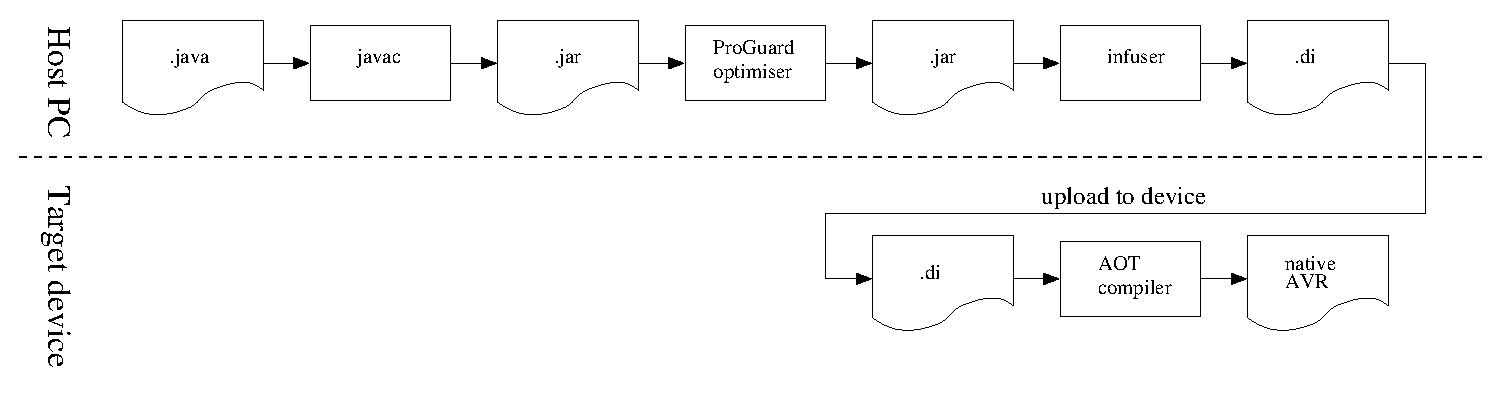
\includegraphics[width=\linewidth]{compilation-process.eps}
  \caption{Java to native AVR compilation}
  \label{fig-translation-process}
\end{figure}

% TODO: clarify two terms: compile-time (javac/proguard/infuser) and translation-time (the VM), and scan the whole text to make sure they're used consistently.

The process from Java source to a native application on the node is shown in Figure \ref{fig-translation-process}.

Like all sensor node JVMs, Darjeeling uses a modified JVM bytecode. Java source code is first compiled to normal Java classes, which are optimised by ProGuard \cite{proguard}. The optimised Java classes are then transformed into Darjeeling's own format, called an 'infusion'. For details of this transformation we refer to the Darjeeling paper \cite{Brouwers:2009cj}. Here it is sufficient to know that the bytecode is modified to make it more suitable for execution on a tiny device, for example by adding 16-bit versions of most operations, but the result remains very similar to standard JVM bytecode. It is also important to note that no knowledge of the target platform is used in this transformation, so the result is still platform independent. This infusion is then sent to the node, where it is translated to native AVR code at load time.

We made several modifications to Darjeeling's infuser and bytecode format to support our AOT compiler and improve performance. These changes will be introduced in more detail in the following sections, but for completeness we also list them here:

\begin{itemize}
	\item the \mycode{BRTARGET} opcode, used to mark targets of branch instructions and modified all branch instructions to target a \mycode{BRTARGET} id instead of a bytecode offset
	\item the \mycode{MARKLOOP} opcode to mark inner loops and the variables it uses
	\item added \mycode{\_FIXED} versions of the \mycode{GETFIELD\_A} and \mycode{PUTFIELD\_A} opcodes, used to access an object's reference fields when the offset is known at compile time
	\item the \mycode{SIMUL} opcode for 16x16-bit to 32-bit multiplication
	\item modified array access opcodes to use 16-bit indexes
	\item added \mycode{\_CONST} versions of the bit shift opcodes to support constant shifts
	\item the \mycode{INVOKELIGHT} opcode for an optimised 'lightweight' way of calling methods
\end{itemize}

\subsection{Goals and limitations}
Working on resource-constrained devices means we have to make some compromises. Our main goal is to build a VM that will produce code that both performs well, and adds as little code size overhead as possible. In addition, we want our VM to fit as many scenarios as possible. We would like to be able to support scenarios were multiple applications may be running on a single device, so when new code is being loaded, the impact on other applications should be as small as possible.

Therefore, the translation process should be very light weight. Specifically, it	 should use as little memory as possible, since memory is a very scarce resource. This means we cannot do any analysis on the bytecode that would require us to hold complex data structures in memory. When receiving a large programme, we should not have to keep multiple messages in memory, but will free each message, which can be as small as a single JVM instruction, immediately after processing.

Since messages do need to be processed in the correct order, the actual transmission protocol may still decide to keep more messages in memory to reduce the need for retransmissions in the case of out of order delivery. But our translation process does not require it to do so, and a protocol that values memory usage over retransmissions cost could simply discard out of order messages and request retransmissions when necessary.

Bytecode instructions are processed in a single pass, one instruction at a time. Only some small, fixed-size data structures are kept in memory during the process. A second pass over the generated code then fills in addresses left blank by branch instructions, since the target addresses of forward branches are not known until the target instruction is generated.

The two metrics we compromise on are load time and code size. Compiling to native code takes longer than simply storing bytecode and starting the interpreter, but we feel this load time delay will be acceptable in many cases, and will be quickly compensated for by improved run-time performance. Native code is also larger than JVM bytecode. This is the price we pay for increased performance, but the optimisations we propose do significantly reduce this code size overhead compared to previous work, thus reducing an important drawback of AOT compilation.

Since our compiler is based on Darjeeling, we share its limitations, most notably a lack of floating point support and reflection. In addition, we do not support threads or exceptions because after compilation to native code, we lose the interpreter loop as a convenient place to switch between threads or unwind the stack to jump to an exception handler. Threads and exceptions have been implemented before on a sensor node AOT compiler \cite{Ellul:2012thesis}, proving it is possible to add support for both, but we feel the added complexity in an environment where code space is at a premium makes other, more lightweight models for concurrency and error handling more appropriate.

\subsection{Translating bytecode to native code}
\label{sec-basic-translation}
The basic approach to translate bytecode to native code on a sensor node was first described by Ellul and Martinez \cite{Ellul:2010iw}. When we receive a bytecode instruction, we simply replace it with an equivalent sequence of native instructions, using the native stack to mimic the JVM stack. An example is shown in Table 1.

The first column shows a fragment of JVM code which does a shift right of variable \mycode{A}, and repeats this while \mycode{A} is greater than \mycode{B}. While not a very practical function, it is the smallest example that will allow us to illustrate our code generation optimisations. The second column shows the code the AOT compiler will execute for each JVM instruction. Together, the first and second column match the case labels and body of a big switch statement in our compiler. The third column shows the resulting AVR native code, which is currently almost a 1-on-1 mapping, with the exception of the branch and some small optimisations by a simple peephole optimiser, both described below.

The example has been slightly simplified for readability. Since the AVR is an 8-bit CPU, in the real code many instructions are duplicated for loading the high and low bytes of a short. The cycle count is based on the actual number of generated instructions, and for a single iteration.

\begin{table}[]
\centering
\caption{Translation of \mycode{ do\{A{>}{>}{>}=1;\} while(A>B);}}
\label{tbl-basic-translation}
\small
\begin{tabular}{llll}
\toprule
JVM & AOT compiler & AVR & cycles \\
\hline
0: BRTARGET(0)   & \sccomment{record current addr} &                &   \\
1: SLOAD\_0      & emit\_LDD(R1,Y+0)        & LDD R1,Y+0     & 4 \\
                 & emit\_PUSH(R1)           & PUSH R1        & 4 \\
2: SCONST\_1     & emit\_LDI(R1,1)          & LDI R1,1       & 2 \\
                 & emit\_PUSH(R1)           & MOV R2,R1      & 1 \\
3: SUSHR         & emit\_POP(R2)            &                &   \\
                 & emit\_POP(R1)            & POP R1         & 4 \\
                 & emit\_RJMP(+2)           & RJMP +2        & 2 \\
                 & emit\_LSR(R1)            & LSR R1         & 2 \\
                 & emit\_DEC(R2)            & DEC R2         & 2 \\
                 & emit\_BRPL(-2)           & BRPL -2        & 3 \\
                 & emit\_PUSH(R1)           &                &   \\
4: SSTORE\_0     & emit\_POP(R1)            &                &   \\
                 & emit\_STD(Y+0,R1)        & STD Y+0,R1     & 4 \\
5: SLOAD\_0      & emit\_LDD(R1,Y+0)        & LDD R1,Y+0     & 4 \\
                 & emit\_PUSH(R1)           & PUSH R1        & 4 \\
6: SLOAD\_1      & emit\_LDD(R1,Y+2)        & LDD R1,Y+2     & 4 \\
                 & emit\_PUSH(R1)           &                &   \\
7: IF\_SCMPGT 0: & emit\_POP(R1)            &                &   \\
                 & emit\_POP(R2)            & POP R2         & 4 \\
                 & emit\_CP(R1,R2)          & CP R1,R2       & 2 \\
                 & emit\_branchtag(GT,0)    & BRGT 0:        & 2 (taken), \\
                 &                          &                & or 1 (not taken) \\
\bottomrule
\end{tabular}
\end{table}



\subsubsection{Branches}
Forward branches pose a problem for our direct translation approach since the target address is not yet known. A second problem is that on the ATmega, a branch may take 1 to 3 words, depending on the distance to the target, so it is also not known how much space should be reserved for a branch.

To solve this the infuser modifies the bytecode by inserting a new instruction, \mycode{BRTARGET}, in front of any instruction that is the target of a branch. The branch instructions themselves are modified to target a branch target id instead of a bytecode offset. When we encounter a \mycode{BRTARGET} during compilation, we do not emit any code, but record the address where the next instruction will be emitted in a separate part of flash. When we encounter a branch instruction, we emit a temporary 3-word 'branch tag' instead, containing the branch target id and the branch condition. After code generation is finished and all target addresses are known, we scan the code again to replace each branch tag with the real branch instruction.

There is still the matter of the different sizes a branch may take. We could simply add \mycode{NOP} instructions to smaller branches to keep the size of each branch at 3 words, but this causes a performance penalty on small, non-taken branches. Instead, we do another scan of the code, before replacing the branch tags, and update the branch target addresses to compensate for cases where a smaller branch will be used. This second scan adds about 500 bytes to the VM, but improves performance, especially on benchmarks where branches are common.

This is an example of something we often see: an optimisation may take a few hundred bytes to implement, but its usefulness may depend on the characteristics of the code being run. In this work we usually decided to implement these optimisations, since they often also result in smaller generated code.

\subsection{Darjeeling split-stack architecture}
\begin{figure}[]
  \includegraphics[width=0.5\linewidth]{object-and-stack-frame-layout.eps}
  \caption{Object and stack frame layout}
  \label{fig-object-and-stack-frame-layout}
\end{figure}

% todo explain one stack for ints on the native stack and another for refs in the frame

In our AOT compiler we use the native stack for the JVM integer operand stack, while space for the reference stack is reserved in the stack frame. This uses less memory than having the integer stack in the stack frame, since we need to reserve space for the maximum stack depth in the frame, which is often much lower for the reference stack than for the integer stack. We use the AVR's X register as a stack pointer for the reference stack.

\subsection{Target platforms}
The AVR family of CPUs is widely used in low power embedded systems. We implemented our VM for the ATmega128 CPU. However, our approach does not depend on any AVR specific properties and we expect similar results for many other CPUs in this class. The main requirements are the ability to reprogramme its own programme memory, and the availability of a sufficient number of registers.

The ATmega128 has 32 8-bit registers. We ran several experiments where we restrict the number of registers our VM may use. As is often the case with caches, we found the first few available registers to have the largest impact, while the added improvement gets less for each added register. Based on this we expect the Cortex M0, with 12 32-bit general purpose registers, or the MSP430, with 12 16-bit registers, and used by Ellul and Martinez \cite{Ellul:2010iw}, to both be good matches as well.

%TODO refer to evaluation 8/16/32 bit and number of regs

\section{Constraints}

Refer back to WuKong here (Section \ref{sec-state-of-the-art-wukong}. Motivation for using as little memory as possible: we want to keep other components running when a new wuclass arrives.

Go as low as possible. Many things to do on a device, can't spend all on reprogramming.

%TODO: references for M0 and MSP430?








\chapter{Optimisations}
\label{sec-optimisations}
Having introduced our baseline AOT compiler, in this chapter we propose several optimisations to improve its performance and reduce the size of the generated code. We will first analyse the difference sources of overhead, and discuss how to reduce each of them.


\section{Sources of overhead}
The performance of our baseline approach is still far behind that of optimised native C. To improve performance, it is important to identify the causes of this overhead. The main sources of overhead we found are:
\begin{itemize}
	\item Lack of optimisations in the Java compiler
	\item AOT code generation overhead
	\begin{itemize}
		\item Push/pop overhead
		\item Load/store overhead
		\item JVM instruction set limitations
	\end{itemize}
	\item Method call overhead
\end{itemize}

We will briefly discuss each source of overhead below, before introducing optimisations to reduce it.

\subsection{Lack of optimisation in \mycode{javac}}
A first source of overhead comes from the fact that the standard \mycode{javac} compiler does almost no optimisations.  Since the JVM is an abstract machine, there is no clear performance model to optimise for. Run-time performance depends greatly on the target platform and the VM implementation running the bytecode, which are unknown when compiling Java source code to JVM bytecode.

The \mycode{javac} compiler simply compiles the code 'as is'. For example, the loop '\mycode{while (a < b*c) \{ a*=2; \}}' will evaluate '\mycode{b*c}' on each iteration, while it is clear that the result will be the same every time.

In most environments this is not a problem because the bytecode is typically compiled to native code before execution, and using knowledge of the target platform and the run-time behaviour, a desktop JIT compiler can make much better decisions than \mycode{javac} could. However, since our AOT compiler simply replaces each instruction with a native equivalent, this leads to significant overhead.

We do use the ProGuard optimiser \cite{proguard}, but this only does very basic optimisations such as method inlining and dead code removal, and does not cover cases such as the example above.

\subsection{AOT translation overhead}
\label{sec-overhead-aot-translation}
Assuming we have high quality JVM bytecode, a second source of overhead comes from the way the bytecode is translated to native code. We distinguish three main types of translation overhead, where the first two are a direct result of the JVM's stack-based architecture.

\subsubsection{Type 1: Pushing and popping values} The compilation process initially results in a large number of push and pop instructions. In our simple example in Table \ref{tbl-basic-translation}, the peephole optimiser was able to eliminate some, but two push/pop pairs remain. For more complex expressions this type of overhead is even higher, since more values will be on the stack at the same time. This means more corresponding push and pop instructions will not be consecutive, and the peephole optimiser cannot eliminate these cases.

\subsubsection{Type 2: Loading and storing values} The second type is also due to the JVM's stack-based architecture. Each operation consumes its operands from the stack, but often the same value is needed again soon after. In this case, because the value is no longer on the stack, we need to do another load, which will result in another read from memory.

In Table \ref{tbl-basic-translation}, it is clear that the \mycode{SLOAD\_0} instruction at label 5 is unnecessary since the value is already in R1.

\subsubsection{Type 3: JVM instruction set limitations} A final source of overhead comes from optimisations that are done in native code, but are not possible in JVM bytecode, at least not in our resource-constrained environment.

The JVM instruction set is very simple, which makes it easy to implement, but this also means some things cannot be expressed as efficiently as in native code. Given enough processing power, compilers can do the complex transformations necessary to make the compiled JVM code run almost as fast as native C, but on a sensor node we do not have such resources and must simply execute the instructions as they are.

In Table \ref{tbl-basic-translation} we see that there is no way to express a single bit shift directly. Instead we have to load the constant 1 onto the stack and execute the generic bit shift instruction. Compare this to addition, where the JVM bytecode does have a special INC instruction to add a constant value to a local variable.

A second example is array access. In JVM bytecode each array access will consume the array reference and index from the stack. When looping over an array, this means we that for each iteration we have to load the reference and index back onto the stack again, and redo the address calculation. In contrast, the native C version would typically just slide a pointer over the array.

\subsection{Method call overhead}
\label{sec-overhead-method-call}
The final source of overhead comes from method calls. In the JVM, each method has a stack frame (or 'activation frame') which the language specification describes as
\begin{quotation}
"containing the target reference (if any) and the argument values (if any), as well as enough space for the local variables and stack for the method to be invoked and any other bookkeeping information that may be required by the implementation (stack pointer, program counter, reference to previous activation frame, and the like)" \cite{Gosling:2014}
\end{quotation}

Darjeeling's stack frame layout was shown in Figure \ref{fig-object-and-stack-frame-layout}. Initialising this complete structure is significantly more work than a native C function call has to do, which may not need a stack frame at all if all the work can be done in registers. Below we list the steps Darjeeling goes through to invoke a Java method:

\begin{enumerate}
  \small
  \item flush the stack cache so parameters are in memory and clear value tags (see sections \ref{sec-optimisations-simple-stack-caching} and \ref{sec-optimisations-popped-value-caching})
  \item save int and ref stack pointers (SP and X)
  \item call the VM's \mycode{callMethod} function, which will:
  \begin{enumerate}
    \item allocate memory for the callee's frame
    \item initialise the callee's frame
    \item pass parameters: pop them off the caller's stack and copy them into the callee's locals
    \item activate the callee's frame: set the VM's active frame pointer to the callee
    \item lookup the address of the AOT compiled code
    \item do the actual \mycode{CALL}, which will return any return value in registers R22 and higher
    \item reactivate the old frame: set the VM's active frame pointer back to the caller
    \item return to the caller's AOT compiled code the return value (if any) in R22 and higher
  \end{enumerate}
  \item restore stack pointer and X register
  \item push the return value onto the stack (using stack caching this will be free)
\end{enumerate}

Even after considerable effort optimising this process, this requires roughly 550 cycles for the simplest case: a call to a static method without any parameters or return value. For a virtual method the cost is higher because we need to look up the right implementation. While we may be able to save some more cycles with an even more rigorous refactoring, it is clear that the number of steps involved will always take considerably more time than a native function call.

\subsection{Optimisations}
\label{sec-optimisations-java-source}
Having identified these sources of overhead, we will use the next three sections to describe the set of optimisations we use to address them. Table \ref{tbl-optimisations-overview} lists each optimisation, and the source of overhead it aims to reduce. The following sections will discuss each optimisation in detail.

\begin{table*}[hbt]
\centering
\caption{List of optimisations per overhead source}
\label{tbl-optimisations-overview}
\small
\begin{tabular}{lll}
\toprule
& Source of overhead & Optimisation \\
\hline
Section \ref{sec-optimisations-manual-java-source-optimisation} &
Lack of optimisations in \mycode{javac}        & Manual optimisation of Java source code \\

Section \ref{sec-optimisations-aot-translation-overhead} &
AOT translation overhead                       & \\
&\hspace{.5cm} Push/pop overhead                & Improved peephole optimiser \\
&                                               & Stack caching \\
&\hspace{.5cm} Load/store overhead              & Popped value caching \\
&                                               & Mark loops \\
&\hspace{.5cm} JVM instruction set limitations  & \mycode{SIMUL} instruction \\
&                                               & \mycode{GET/PUTFIELD\_A\_FIXED} instructions \\
&                                               & constant shift optimisation \\
&                                               & 16-bit array indexes \\

Section \ref{sec-optimisations-method-calls} &
Method call overhead                           & \mycode{INVOKELIGHT} instruction \\
\bottomrule
\end{tabular}
\end{table*}




\section{Manually optimising the Java source code}
\label{sec-optimisations-manual-java-source-optimisation}
As shown in Figure \ref{fig-translation-process}, our current implementation uses three steps to translate Java source code to CapeVM bytecode: the standard Java compiler, the ProGuard optimiser, and the modified Darjeeling infuser. None of these do any complex optimisations. 

In a future version, these three steps should be merged into an 'optimising infuser' which uses all the normal, well-known optimisation techniques to produce better quality bytecode, but at the moment we do not have the resources to build such an optimising infuser.

Since our goal is to determine what level of performance is possible on a sensor node, the Java source was manually optimised to get better quality JVM bytecode from \mycode{javac}. While these changes are not an automatic optimisation we developed, we find it important to mention them explicitly and analyse their impact, since many developers may expect these optimisations to happen automatically and without this step it would be impossible to reproduce our results.

% We have been careful to limit ourselves to 'fair' optimisations, by which we mean optimisations that an optimising infuser could reasonably be expected to do automatically, given some basic, conservative assumptions about the performance model. 

The most common optimisations that were done are:
\begin{itemize}
	\item Store the result of expressions calculated in a loop in a temporary variable, if it is known the result will be the same for each iteration.
	\item Since array and object field access is relatively expensive and not cached by the mark loop optimisation discussed in Section \ref{sec-optimisation-markloops}, prefer to minimise array and object access by using a temporary local variable, if the value may be used again soon.
	\item Manually inline \texttt{\#define}s and functions that were inlined by \mycode{avr-gcc} in the C version of the benchmark.
	\item Use 16-bit variables for array indexes where possible.
	\item Use bit shifts for multiplication and division by a power of two.
\end{itemize}

We will examine the effect of some other optimisations on the \mybench{CoreMark} benchmark in Section \ref{sec-evaluation-coremark}.

\paragraph{Temporary variables}
The first two optimisations generate extra store instructions, which means they may not always be beneficial if the value is never used again. However, a value often only needs to be reused only once for it to be faster to store it in a local variable than to calculate it twice or do two array accesses. If we use the mark loops optimisation discussed in Section \ref{sec-optimisation-markloops}, in many cases the variable may be stored in registers, making accessing them either very cheap, or completely free.

\paragraph{Manual inlining}
ProGuard automatically inlines methods that are only called from a single location, or small methods called from multiple locations. In these cases it simply replaces the \mycode{INVOKE} instruction with the callee's body, prepended with \mycode{STORE} instructions to pop the parameters off the stack and initialise the callee's local variables.

Manual inlining often results in better code because it may not be necessary to store the parameters in local variables if they are only used once. We therefore manually inline all small methods that were either a \texttt{\#define} in the C version of our benchmarks, or a function that was inlined by \mycode{avr-gcc}. Again, it is easy to imagine that an optimising infuser should be able to come to the same result automatically.



\paragraph{Platform independence}
Assuming an optimising infuser does raise the question how platform independent the resulting code is. If the infuser has more specific knowledge about the target platform, it can produce better code for that platform, but, while it should still run anywhere, this may not be as efficient on other platforms.

The optimisations described here are based on very conservative assumptions, and are not specific to the ATmega CPU. Therefore, they should work well for most programmes, independent of the hardware they are running on.

\paragraph{Example} Listing \ref{lst-manual-optimisation} shows an example of these manual optimisations, applied to the \mybench{bubble sort} benchmark. To have a fair comparison, we applied exactly the same optimisations to the C versions of our benchmarks, but here this had little or no effect on the performance.

\begin{listing}
\centering

\begin{minipage}[t]{0.47\textwidth}
\centering
  \begin{minted}{java}
// ORIGINAL
public static void bsort(int[] numbers)
{
  short NUMBERS=(short)numbers.length;
  for (short i=0; i<NUMBERS; i++)
  {
    for (short j=0; j<NUMBERS-i-1; j++)
    {
      if (numbers[j]>numbers[j+1])
      {
        int temp = numbers[j];
        numbers[j] = numbers[j+1];
        numbers[j+1] = temp;
      }
    }
  }
}
\end{minted}
\end{minipage}
\hfill
\begin{minipage}[t]{0.52\textwidth}
\centering
\begin{minted}[linenos=false]{java}
// MANUALLY OPTIMISED
public static void bsort(int[] numbers)
{
  short NUMBERS=(short)numbers.length;
  for (short i=0; i<NUMBERS; i++)
  {
    short x=(short)(NUMBERS-i-1);
    short j_plus_1 = 1;
    for (short j=0; j<x; j++)
    {
      int val_at_j = numbers[j];
      int val_at_j_plus_1 = numbers[j_plus_1];
      if (val_at_j>val_at_j_plus_1)
      {
        numbers[j] = val_at_j_plus_1;
        numbers[j_plus_1] = val_at_j;
      }
      j_plus_1++;
    }
  }
}
\end{minted}
\end{minipage}
\caption{Optimisation of the bubble sort benchmark}
\label{lst-manual-optimisation}
\end{listing}



\section{AOT translation overhead}
\label{sec-optimisations-aot-translation-overhead}
Now that we have good quality bytecode to work with, we can start addressing the overhead incurred during the AOT compilation process.

\subsection{Improving the peephole optimiser}
\label{sec-improved-peephole}

Our first optimisation is a small but effective extension to the simple peephole optimiser. Instead of optimising only consecutive push/pop pairs, we can optimise any pair of push/pop instructions if the following holds for the instructions in between:
%\begin{itemize}
%	\item they contain the same number of \mycode{push} and \mycode{pop} instructions (the \mycode{pop} matches the \mycode{push})
%	\item they contain no branches
%	\item they may be do not use the \emph{target} register of the \mycode{pop}
%\end{itemize}

\begin{listing}[H]
 \centering
 \begin{minted}[fontsize=\scriptsize]{asm}
PUSH Rs
..
..       instructions in between: - contain the same number of push and pop instructions
..                                - contain no branches
..                                - do not use register Rd
..
POP  Rd
 \end{minted}
\end{listing}

In this case the pair can be eliminated if \mycode{Rs} == \mycode{Rd}, otherwise it is replaced by a '\mycode{mov Rd, Rs}'. Two push/pop pairs remained in our earlier example Table \ref{tbl-basic-translation}. For the pair in instructions 5 and 7, the value is popped into register R2. Since instruction 6 does not use register R2, we can safely replace this pair with a direct move. In contrast, the pair in instructions 1 and 3 cannot be optimised since the value is popped into register R1, which is also used by instruction 2.

% This optimisation adds 278 bytes to the optimiser, since it now needs to understand the bytecode well enough to determine which registers are being used.

\subsection{Simple stack caching}
\label{sec-optimisations-simple-stack-caching}
\begin{table*}[hbt]
\centering
\caption{Simple stack caching}
\label{tbl-simplestackcaching}
\scriptsize
\addtolength{\tabcolsep}{-2pt}
\begin{tabular}{llll|c|c|c}
\toprule
JVM                & AOT compiler                                         & AVR                 & cycles & cache state R1                   & cache state R2                   & cache state R3                   \\
\hline
0: BRTARGET(0)     & \sccomment{record current addr} & & & & & \\
1: SLOAD\_0        & operand\_1 = sc\_getfreereg()                        &                     &        & \stackcacheentry{    }{   }{   } & \stackcacheentry{    }{   }{   } & \stackcacheentry{    }{   }{   } \\
                   & emit\_LDD(operand\_1,Y+0)                            & LDD R1,Y+0          & 4      & \stackcacheentry{    }{   }{   } & \stackcacheentry{    }{   }{   } & \stackcacheentry{    }{   }{   } \\
                   & sc\_push(operand\_1)                                 &                     &        & \stackcacheentry{Int1}{   }{   } & \stackcacheentry{    }{   }{   } & \stackcacheentry{    }{   }{   } \\
3: SUSHR\_CONST(1) & operand\_1 = sc\_pop()                               &                     &        & \stackcacheentry{    }{   }{   } & \stackcacheentry{    }{   }{   } & \stackcacheentry{    }{   }{   } \\
                   & emit\_LSR(operand\_1)                                & LSR R1              & 2      & \stackcacheentry{    }{   }{   } & \stackcacheentry{    }{   }{   } & \stackcacheentry{    }{   }{   } \\
                   & sc\_push(operand\_1)                                 &                     &        & \stackcacheentry{Int1}{   }{   } & \stackcacheentry{    }{   }{   } & \stackcacheentry{    }{   }{   } \\
4: SSTORE\_0       & operand\_1 = sc\_pop()                               &                     &        & \stackcacheentry{    }{   }{   } & \stackcacheentry{    }{   }{   } & \stackcacheentry{    }{   }{   } \\
                   & emit\_STD(Y+0,operand\_1)                            & STD Y+0,R1          & 4      & \stackcacheentry{    }{   }{   } & \stackcacheentry{    }{   }{   } & \stackcacheentry{    }{   }{   } \\
5: SLOAD\_0        & operand\_1 = sc\_getfreereg()                        &                     &        & \stackcacheentry{    }{   }{   } & \stackcacheentry{    }{   }{   } & \stackcacheentry{    }{   }{   } \\
                   & emit\_LDD(operand\_1,Y+0)                            & LDD R1,Y+0          & 4      & \stackcacheentry{    }{   }{   } & \stackcacheentry{    }{   }{   } & \stackcacheentry{    }{   }{   } \\
                   & sc\_push(operand\_1)                                 &                     &        & \stackcacheentry{Int1}{   }{   } & \stackcacheentry{    }{   }{   } & \stackcacheentry{    }{   }{   } \\
6: SLOAD\_1        & operand\_1 = sc\_getfreereg()                        &                     &        & \stackcacheentry{Int1}{   }{   } & \stackcacheentry{    }{   }{   } & \stackcacheentry{    }{   }{   } \\
                   & emit\_LDD(operand\_1,Y+2)                            & LDD R2,Y+2          & 4      & \stackcacheentry{Int1}{   }{   } & \stackcacheentry{    }{   }{   } & \stackcacheentry{    }{   }{   } \\
                   & sc\_push(operand\_1)                                 &                     &        & \stackcacheentry{Int2}{   }{   } & \stackcacheentry{Int1}{   }{   } & \stackcacheentry{    }{   }{   } \\
7: IF\_SCMPGT 0:   & operand\_1 = sc\_pop()                               &                     &        & \stackcacheentry{Int1}{   }{   } & \stackcacheentry{    }{   }{   } & \stackcacheentry{    }{   }{   } \\
                   & operand\_2 = sc\_pop()                               &                     &        & \stackcacheentry{    }{   }{   } & \stackcacheentry{    }{   }{   } & \stackcacheentry{    }{   }{   } \\
                   & emit\_CP(operand\_1, operand\_2);                    & CP R2,R1            & 2      & \stackcacheentry{    }{   }{   } & \stackcacheentry{    }{   }{   } & \stackcacheentry{    }{   }{   } \\
                   & emit\_branchtag(GT, 0);                              & BRGT 0:             & 2 or 1 & \stackcacheentry{    }{   }{   } & \stackcacheentry{    }{   }{   } & \stackcacheentry{    }{   }{   } \\
\bottomrule
\end{tabular}
\addtolength{\tabcolsep}{2pt}
\end{table*}


The improved peephole optimiser can remove part of the type 1 overhead, but still many cases remain where it cannot eliminate the push/pop instructions. We use a form of stack caching \cite{Ertl:1995dv} to eliminate most of the remaining push/pop overhead. Stack caching is not a new technique, originally proposed for Forth interpreters in 1995. But the tradeoffs involved are very different depending on the scenario it is applied in, and it turns out to be exceptionally well suited for a sensor node AOT compiler:

First, the VM in the original paper is an interpreter, which means the stack cache has to be very lightweight, or the overhead from managing it at run-time will outweigh the time saved by reducing memory accesses. Since we only need to keep track of the cache state at load time, this restriction does not apply for an AOT compiler and we can afford to spend more time managing it. Second, the simplicity of the approach means it requires very little memory: only 11 bytes of RAM and less than 1KB of code more than the peephole optimiser.

The basic idea of stack caching is to keep the top elements of the stack in registers instead of main memory. We add a cache state to our VM to keep track of which registers are holding stack elements. For example, if the top two elements are kept in registers, an ADD instruction does not need to access main memory, but can simply add these registers, and update the cache state. Values are only spilled to memory when all registers available for stack caching are in use.

In the baseline AOT approach, each JVM instruction maps to a fixed sequence of native instructions that always use the same registers. Using stack caching, the registers are controlled by a stack cache manager that provides three functions:
\begin{itemize}
    \item \mycode{getfree}: Instructions such as load instructions will need a free register to load the value into, which will later be pushed onto the stack. If all registers are in use, \mycode{getfree} spills the register that's lowest on the stack to memory by emitting a \mycode{PUSH}, and then returns that register. This way the top of the stack is kept in registers, while lower elements may be spilled to memory.
    \item \mycode{pop}: Pops the top element off the stack and tells the code generator in which register to find it. If stack elements have previously been spilled to main memory and no  elements are left in registers, \mycode{pop} will emit a real \mycode{POP} instruction to get the value back from memory.
    \item \mycode{push}: Updates the cache state so the passed register is now at the top of the stack. This should be a register that was previously returned by \mycode{getfree}, or \mycode{pop}.
\end{itemize}

Using stack caching, code generation is split between the instruction translator, which emits the instructions that do the actual work, and the cache manager which manages the registers and may emit code to spill stack elements to memory, or to retrieve them again. But as long as enough registers are available, it will only manipulate the cache state.

In Table \ref{tbl-simplestackcaching} we translate the same example we used before, but this time using stack caching. To save space, Table \ref{tbl-simplestackcaching} also includes the constant shift optimisation described in Section \ref{sec-opt-constant-shift}. The \mycode{emit\_PUSH} and \mycode{emit\_POP} instructions have been replaced by calls to the cache manager, and instructions that load something onto the stack start by asking the cache manager for a free register. The state of the stack cache is shown in the three columns added to the right. Currently it only tracks whether a register is on the stack or not. "Int1" marks the top element, followed by "Int2", etc. (this example does not use the reference stack) In the next two optimisations we will extend the cache state further.
 
The example only shows three registers, but the ATmega128 we use has 32 8-bit registers. Since Darjeeling uses a 16-bit stack, we manage them as pairs. 10 registers are reserved, for example as a scratch register or to store a pointer to local or static variables, leaving 11 pairs available for stack caching.

\paragraph{Branches} Branch targets may be reached from multiple locations. We know the cache state if it was reached from the previous instruction, but not if it was reached through a branch. To ensure the cache state is the same on both paths, we flush the whole stack to memory whenever we encounter either a branch or a \mycode{BRTARGET} instruction. 

This may seem bad for performance, but fortunately in the code generated by \mycode{javac} the stack is empty at almost all branches. The exception is the ternary \mycode{?} \mycode{:} operator, which may cause a conditional branch with elements on the stack, but in most cases flushing at branches and branch targets does not result in any extra overhead.

\subsection{Popped value caching}
\label{sec-optimisations-popped-value-caching}
Stack caching can eliminate most of the push/pop overhead, even when the stack depth increases. We now turn our attention to reducing the overhead resulting from load and store instructions.

\begin{table*}[hbt]
\centering
\caption{Popped value caching}
\label{tbl-poppedvaluecaching}
\scriptsize
\addtolength{\tabcolsep}{-2pt}
\begin{tabular}{llll|c|c|c}
\toprule
JVM                & AOT compiler                                         & AVR                 & cycles & cache state R1                   & cache state R2                   & cache state R3                   \\
\hline
0: BRTARGET(0)   & \sccomment{record current addr} & & & & & \\
1: SLOAD\_0        & operand\_1 = sc\_getfreereg()                        &                     &        & \stackcacheentry{    }{   }{   } & \stackcacheentry{    }{   }{   } & \stackcacheentry{    }{   }{   } \\
                   & emit\_LDD(operand\_1,Y+0)                            & LDD R1,Y+0          & 4      & \stackcacheentry{    }{   }{   } & \stackcacheentry{    }{   }{   } & \stackcacheentry{    }{   }{   } \\
                   & sc\_push(operand\_1)                                 &                     &        & \stackcacheentry{Int1}{LS0}{   } & \stackcacheentry{    }{   }{   } & \stackcacheentry{    }{   }{   } \\
3: SUSHR\_CONST(1) & operand\_1 = sc\_pop\_destructive()                  &                     &        & \stackcacheentry{    }{   }{   } & \stackcacheentry{    }{   }{   } & \stackcacheentry{    }{   }{   } \\
                   & emit\_LSR(operand\_1)                                & LSR R1              & 2      & \stackcacheentry{    }{   }{   } & \stackcacheentry{    }{   }{   } & \stackcacheentry{    }{   }{   } \\
                   & sc\_push(operand\_1)                                 &                     &        & \stackcacheentry{Int1}{   }{   } & \stackcacheentry{    }{   }{   } & \stackcacheentry{    }{   }{   } \\
4: SSTORE\_0       & operand\_1 = sc\_pop\_tostore()                      &                     &        & \stackcacheentry{    }{LS0}{   } & \stackcacheentry{    }{   }{   } & \stackcacheentry{    }{   }{   } \\
                   & emit\_STD(Y+0,operand\_1)                            & STD Y+0,R1          & 4      & \stackcacheentry{    }{LS0}{   } & \stackcacheentry{    }{   }{   } & \stackcacheentry{    }{   }{   } \\
5: SLOAD\_0        & \sccomment{skip codegen, just update cache state}    &                     &        & \stackcacheentry{Int1}{LS0}{   } & \stackcacheentry{    }{   }{   } & \stackcacheentry{    }{   }{   } \\
6: SLOAD\_1        & operand\_1 = sc\_getfreereg()                        &                     &        & \stackcacheentry{Int1}{LS0}{   } & \stackcacheentry{    }{   }{   } & \stackcacheentry{    }{   }{   } \\
                   & emit\_LDD(operand\_1,Y+2)                            & LDD R2,Y+2          & 4      & \stackcacheentry{Int1}{LS0}{   } & \stackcacheentry{    }{   }{   } & \stackcacheentry{    }{   }{   } \\
                   & sc\_push(operand\_1)                                 &                     &        & \stackcacheentry{Int2}{LS0}{   } & \stackcacheentry{Int1}{LS1}{   } & \stackcacheentry{    }{   }{   } \\
7: IF\_SCMPGT 0:   & operand\_1 = sc\_pop\_nondestructive()               &                     &        & \stackcacheentry{Int1}{LS0}{   } & \stackcacheentry{    }{LS1}{   } & \stackcacheentry{    }{   }{   } \\
                   & operand\_2 = sc\_pop\_nondestructive()               &                     &        & \stackcacheentry{    }{LS0}{   } & \stackcacheentry{    }{LS1}{   } & \stackcacheentry{    }{   }{   } \\
                   & emit\_CP(operand\_1, operand\_2);                    & CP R2,R1            & 2      & \stackcacheentry{    }{LS0}{   } & \stackcacheentry{    }{LS1}{   } & \stackcacheentry{    }{   }{   } \\
                   & emit\_branchtag(GT, 0);                              & BRGT 0:             & 2 or 1 & \stackcacheentry{    }{LS0}{   } & \stackcacheentry{    }{LS1}{   } & \stackcacheentry{    }{   }{   } \\
\bottomrule
\end{tabular}
\addtolength{\tabcolsep}{2pt}
\end{table*}



We add a 'value tag' to each register's cache state to keep track of what value is currently held in the register, even after it is popped from the stack. Some JVM instructions have a value tag associated with them to indicate which value or variable they load, store, or modify. Each tag consist of a tuple (type, datatype, number). For example, the JVM instructions \mycode{ILOAD\_0} and \mycode{ISTORE\_0}, which load and store the local integer variable with id 0, both have tag LI0, short for (local, int, 0). \mycode{SCONST\_1} has tag CS1, or (constant, short, 1), etc. These tags are encoded in a 16-bit value.

We add a function, \mycode{sc\_can\_skip}, to the cache manager. This function will examine the type of each instruction, its value tag, and the cache state. If it finds that we are loading a value that is already present in a register, it updates the cache state to put that register on the stack, and returns true to tell the main loop to skip code generation for this instruction.

Table \ref{tbl-poppedvaluecaching} shows popped value caching applied to our example. At first, the stack is empty. When \mycode{sc\_push} is called, it detects the current instruction's value tag, and marks the fact that R1 now contains LS0. In \mycode{SUSHR\_CONST}, the \mycode{pop} has been changed to \mycode{pop\_destructive}. This tells the cache manager that the value in the register will be destroyed, so the value tag has to be cleared again since R1 will no longer contain LS0. The \mycode{SSTORE\_0} instruction now calls \mycode{pop\_tostore} instead of  \mycode{pop}, to inform the cache manager it will store this value in the variable identified by \mycode{SSTORE\_0}'s value tag. This means the register once again contains LS0. If any other register was marked as containing LS0, the cache manager would clear that tag, since it is no longer accurate after we update the variable.

In line 5, we need to load LS0 again, but now the cache state shows that LS0 is already in R1. This means we do not need to load it from memory, but just update the cache state so that R1 is pushed onto the stack. At run-time this \mycode{SLOAD\_0} will have no cost at all.

There are a few more details to get right. For example if we load a value that's already on the stack, we generate a move to copy it. When \mycode{sc\_getfree} is called, it will try to return a register without a value tag. If none are available, the least recently used register is returned. This is done to maximise the chance we can reuse a value later, since recently used values are more likely to be used again.

\paragraph{Branches} As we do not know the state of the registers if an instruction is reached through a branch, we have to clear all value tags when we pass a \mycode{BRTARGET} instruction, meaning that any new loads will have to come from memory. At branches we can keep the value tags, because if the branch is not taken, we do know the state of the registers in the next instruction.

\subsection{Mark loops}
\label{sec-optimisation-markloops}
\begin{table*}[hbt]
\centering
\caption{Mark loops}
\label{tbl-markloop}
\scriptsize
\addtolength{\tabcolsep}{-2pt}
\begin{tabular}{llll|c|c|c}
\toprule
JVM                & AOT compiler                                            & AVR                 & cycles & cache state R1                      & cache state R2                      & cache state R3                   \\
\hline
0: MARKLOOP(0,1)   & \emph{ << emit markloop prologue:}                      & LDD R1,Y+0          & 4      & \stackcacheentry{    }{LS0}{PIN   } & \stackcacheentry{    }{   }{      } & \stackcacheentry{    }{   }{   } \\
                   &  \emph{\hspace{.7cm}LS0 and LS1 are live >> }           & LDD R2,Y+2          & 4      & \stackcacheentry{    }{LS0}{PIN   } & \stackcacheentry{    }{LS1}{PIN   } & \stackcacheentry{    }{   }{   } \\
1: BRTARGET(0)     & \sccomment{record current addr}                         &                     &        & \stackcacheentry{    }{LS0}{PIN   } & \stackcacheentry{    }{LS1}{PIN   } &                                  \\
2: SLOAD\_0        & \sccomment{skip codegen, just update cache state}       &                     &        & \stackcacheentry{Int1}{LS0}{PIN   } & \stackcacheentry{    }{LS1}{PIN   } & \stackcacheentry{    }{   }{   } \\
4: SUSHR\_CONST(1) & operand\_1 = sc\_pop\_destructive()                     & MOV R3,R1           & 1      & \stackcacheentry{    }{LS0}{PIN   } & \stackcacheentry{    }{LS1}{PIN   } & \stackcacheentry{    }{   }{   } \\
                   & emit\_LSR(operand\_1)                                   & LSR R3              & 2      & \stackcacheentry{    }{LS0}{PIN   } & \stackcacheentry{    }{LS1}{PIN   } & \stackcacheentry{    }{   }{   } \\
                   & sc\_push(operand\_1)                                    &                     &        & \stackcacheentry{    }{LS0}{PIN   } & \stackcacheentry{    }{LS1}{PIN   } & \stackcacheentry{Int1}{   }{   } \\
5: SSTORE\_0       & \sccomment{skip codegen, move to pinned reg}            & MOV R1,R3           & 1      & \stackcacheentry{    }{LS0}{PIN   } & \stackcacheentry{    }{LS1}{PIN   } & \stackcacheentry{    }{   }{   } \\
6: SLOAD\_0        & \sccomment{skip codegen, just update cache state}       &                     &        & \stackcacheentry{Int1}{LS0}{PIN   } & \stackcacheentry{    }{LS1}{PIN   } & \stackcacheentry{    }{   }{   } \\
7: SLOAD\_1        & \sccomment{skip codegen, just update cache state}       &                     &        & \stackcacheentry{Int2}{LS0}{PIN   } & \stackcacheentry{Int1}{LS1}{PIN   } & \stackcacheentry{    }{   }{   } \\
8: IF\_SCMPGT 0:   & operand\_1 = sc\_pop\_nondestructive()                  &                     &        & \stackcacheentry{Int1}{LS0}{PIN   } & \stackcacheentry{    }{LS1}{PIN   } & \stackcacheentry{    }{   }{   } \\
                   & operand\_2 = sc\_pop\_nondestructive()                  &                     &        & \stackcacheentry{    }{LS0}{PIN   } & \stackcacheentry{    }{LS1}{PIN   } & \stackcacheentry{    }{   }{   } \\
                   & emit\_CP(operand\_1, operand\_2);                       & CP R2,R1            & 2      & \stackcacheentry{    }{LS0}{PIN   } & \stackcacheentry{    }{LS1}{PIN   } & \stackcacheentry{    }{   }{   } \\
                   & emit\_branchtag(GT, 0);                                 & BRGT 1:             & 2 or 1 & \stackcacheentry{    }{LS0}{PIN   } & \stackcacheentry{    }{LS1}{PIN   } & \stackcacheentry{    }{   }{   } \\
9: MARKLOOP(end)   & \sccomment{emit markloop epilogue: LS0 is live}         & STD Y+0,R1          & 4      & \stackcacheentry{    }{LS0}{      } & \stackcacheentry{    }{LS1}{      } & \stackcacheentry{    }{   }{   } \\
\bottomrule
\end{tabular}
\addtolength{\tabcolsep}{2pt}
\end{table*}


Popped value caching reduces the type 2 overhead significantly, but the fact that we have to clear the value tags at branch targets means that a large part of that overhead still remains. This is particularly true for loops, since each iteration often uses the same variables, but the branch to start the next iteration clears those values from the stack cache. This is addressed by the next optimisation.

Again, we modify the infuser to add a new instruction to the bytecode: \mycode{MARKLOOP}. This instruction is used to mark the beginning and end of each inner loop. \mycode{MARKLOOP} has a larger payload than most JVM instructions: it contains a list of value tags that will appear in the loop and how often each tag appears, sorted in descending order.

When we encounter the \mycode{MARKLOOP} instruction, the VM may decide to reserve a number of registers and pin the most frequently used local variables to them. If it does, code is generated to prefetch these variables from memory and store them in registers. While in the loop, loading or storing these pinned variables does not require memory access, but only a manipulation of the cache state, and possibly a simple move between registers. However, these registers will no longer be available for normal stack caching. Since 4 register pairs need to be reserved for code generation, at most 7 of the 11 available pairs can be used by mark loops.

Because the only way to enter and leave the loop is through the \mycode{MARKLOOP} instructions, the values can remain pinned for the whole duration of the block, regardless of the branches made inside. This lets us eliminate more load instructions, and also replace store instructions by a much cheaper move to the pinned register. \mycode{INC} instructions, which increment a local variable, operate directly on the pinned register, saving both a load and a store. All these cases are handled in \mycode{sc\_can\_skip}, bypassing the normal code generation. We also need to make a small change to \mycode{sc\_pop\_destructive}. If the register we're about to pop is pinned, we cannot just return it since it would corrupt the value of the pinned local variable. Instead we will first emit a move to a free, non-pinned register, and return that instead.

In Table \ref{tbl-markloop} the first instruction is now \mycode{MARKLOOP}, which tells the compiler local short variables 0 and 1 will be used. The compiler decides to pin them both to registers 1 and 2. The \mycode{MARKLOOP} instruction also tells the VM whether or not the variables are live, which they are at this point, so the two necessary loads are generated. This is reflected in the cache state. No elements are on the stack yet, but register 1 is pinned to LS0, and register 2 to LS1.

Next, LS0 is loaded. Since it is pinned to register 1, no code is generated, but the cache state is updated to reflect LS0 is now on top of the stack. Next, \mycode{SUSHR\_CONST} pops destructively. We cannot simply return register 1 since that would corrupt the value of variable LS0, so \mycode{sc\_pop\_destructive} emits a move to a free register and returns that register instead. Since LS0 is pinned, we can also skip \mycode{SSTORE\_0}, but we do need to emit a move back to the pinned register.

The next two loads are straightforward and can be skipped, and in the branch we see the registers are popped non-destructively, so we can use the pinned registers directly.

Finally, we see the loop ends with another \mycode{MARKLOOP}, telling the compiler only local 0 is live at this point. This means we need to store LS0 in register 1 back to memory, but we can skip LS1 since it is no longer needed.

The total cost is now 20 cycles, which appears to be up two from the 18 cycles spent using only popped value caching. But 12 of these are spent before and after the loop, while each iteration now only takes 8 cycles, a significant improvement from the 48 cycles spent in the original version in Table \ref{tbl-basic-translation}.

\subsection{Instruction set modifications}
Next, we introduce four optimisations that target the type 3 overhead: cases where limitations in the JVM instruction set means we cannot express some operations as efficiently as we would like. This type of overhead is the most difficult to address because many of the transformations a desktop VM can do to avoid it take more resources than we can afford on a tiny device. Also, this type of overhead covers many different cases, and optimisations that help in a specific case may not be general enough to justify spending additional resources on it.

Still, there are a few things we can do by modifying the instruction set, that come at little cost to the VM and can make a significant difference.

Darjeeling's original instruction set is already quite different from the normal JVM instruction set. The most important change is the introduction of 16-bit operations. The JVM is internally a 32-bit machine, meaning \mycode{short}, \mycode{byte}, and \mycode{char} are internally stored as 32-bit integers. On a sensor device where memory is the most scarce resource, we often want to use shorter data types. To support this, Darjeeling internally stores values in 16-bit slots, and introduces 16-bit versions of all integer operations. For example if we want to multiply two shorts and store the result in a short, the 32-bit \mycode{IMUL} instruction is replaced by the 16-bit \mycode{SMUL} instruction. These transformations are all done by the infuser (see Figure \ref{fig-translation-process}).

However, the changes made by Darjeeling are primarily aimed at reducing memory consumption, not at improving performance. We extend the infuser to make several other changes. The \mycode{BRTARGET} and \mycode{MARKLOOP} instructions have already been discussed, and the \mycode{INVOKELIGHT} instruction is the topic of the next section. In addition to these, we made the following four other modifications to Darjeeling's instruction set:

\subsubsection{\mycode{GET/PUTFIELD\_A\_FIXED} reference field access}
The \mycode{GETFIELD\_*} and \mycode{PUTFIELD\_*} instructions are used to access fields in objects. Because of Darjeeling's split architecture, the offset from the object pointer is known at compile time only for integer fields, but not for reference fields. As shown in Figure \ref{fig-super-class-sub-class-field-layout}, integer fields will be at the same offset, regardless of whether an object is of the compile-time type, or a subclass. References fields may shift up in subclass instances, so \mycode{GETFIELD\_A} and \mycode{PUTFIELD\_A} must examine the object's actual type and calculate the offset accordingly, adding significant overhead.

\begin{figure}[]
  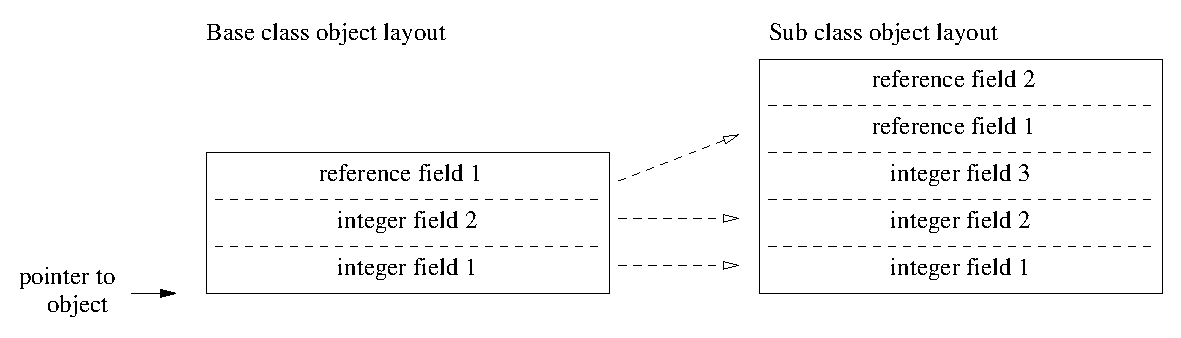
\includegraphics[width=0.6\linewidth]{super-class-sub-class-field-layout.eps}
  \caption{Base class and sub class layout }
  \label{fig-super-class-sub-class-field-layout}
\end{figure}

This overhead can be avoided if we can be sure of the offset at compile time, which is the case if the class is marked \mycode{final}. In this case the infuser will replace the \mycode{GETFIELD\_A} or \mycode{PUTFIELD\_A} opcode with a \mycode{\_FIXED} version so the VM knows it is safe to determine the offset at AOT compile time. Conveniently, one of the optimisations ProGuard does, is marking any class that is not subclassed as \mycode{final}, so most of this is automatic.

\paragraph{Alternative solutions} An alternative we considered is to let go of Darjeeling's split architecture for object fields and mix them, so the offsets for reference fields would also be known at compile time. To allow the garbage collector to find the reference fields we could either extend the class descriptors with a bit map indicating the type of each slot, or let the garbage collector scan all classes in the inheritance line of an object.

We chose our solution because it is easy to implement and adds only a few bytes to the VM size, while the garbage collector is already one of the most complex components of the VM. Also, we found that almost all classes in our benchmark could be marked \mycode{final}. But either solution would work, and the alternative could be considered as a more general solution.

\paragraph{Evaluation}
The impact of this optimisation is significant, but we decided not to include it in our evaluation since the overhead is the result of implementation choices in Darjeeling, which was optimised for size rather than performance. This means the overhead is rather arbitrary, and not a direct result of the AOT techniques or the JVM's design. Therefore, all results reported in this paper are with this optimisation already turned on.

Since Darjeeling's split architecture has a lot of advantages in terms of complexity and VM size, we still feel it is important to mention this as an example of the kind of trade-offs faced when optimising for performance.

\subsubsection{\mycode{SIMUL} 16-bitx16-bit to 32-bit multiplication}
While Darjeeling already introduced 16-bit arithmetic operations, it does not cover the case of multiplying two 16-bit shorts, and storing the result in a 32-bit integer. In this case the infuser would emit \mycode{S2I} instructions to convert the operands to two 32-bit integers, and then use the normal \mycode{IMUL} instruction for full 32-bit multiplication. On a device with a shorter word size, this is significantly more expensive than 16x16 to 32-bit multiplication.

We added a new opcode, \mycode{SIMUL}, for this case, which the infuser will emit if it can determine the operands are 16-bit, but the result is used as a 32-bit integer.

We could added more instructions, for example \mycode{SIADD} instruction for addition, \mycode{BSMUL} for 8-bit to 16-bit multiplication, etc. But there is always a trade-off between the added complexity of an optimisation and the performance improvement it yields, and for these cases this is much smaller than for \mycode{SIMUL}.

\subsubsection{16-bit array indexes}
Normal JVM array access instructions (\mycode{IASTORE}, \mycode{IALOAD}, etc) expect the index operand to be a 32-bit integer. On a sensor node with only a few KB of memory, we will never have arrays that require such large indexes, so we modified the array access instructions to expect a 16-bit index instead. This is easily done in Darjeeling's infuser, which contains a specification of the type of operands of each opcode, and will automatically emit type conversions where necessary.

This complements one of the manual optimisations discussed in Section \ref{sec-optimisations-manual-java-source-optimisation}. Using short values as index variables makes operations on the index variable cheaper, while changing the operand of the array access instructions reduces the amount of work the array access instruction needs to do and the number of registers it requires.

\subsubsection{Constant bit shifts}
\label{sec-opt-constant-shift}
Finally, shifts by a constant number of bits appear in seven of the eight benchmarks described in Section 6. They appear not only in computation intensive benchmarks, but also as optimised multiplications or divisions by a power of 2, which are common in many programmes.

In JVM bytecode the shift operators take two operands from the stack: the value to shift, and the number of bits to shift by. While this is generic, it is not efficient for constant shifts: we first need to push the constant onto the stack, and then the bit shift is implemented as a simple loop which shifts one bit at a time. If we already know the number of bits to shift by, we can generate much more efficient code.

Note that this is different from other arithmetic operations with a constant operand. For operations such as addition, our translation process results in loading the constant and performing the operation, similar to what \mycode{avr-gcc} produces in most cases. An addition takes just as long when the operand is taken from the stack, as when it is a constant. What makes bit shifts a special case is that for an unknown number of bits a loop must be generated to shift one bit at a time, which is much slower than the code we can generate for a shift by a constant number of bits.

We optimise these cases by adding \mycode{\_CONST} versions of the bit shift instructions \mycode{ISHL}, \mycode{ISHR}, \mycode{IUSHR}, \mycode{SSHL}, \mycode{SSHR}, and \mycode{SUSHR}. We add a simple scan to the infuser to find constant loads that are immediately followed by a bit shift. For these cases the constant load is removed, and the bit shift instruction, for example \mycode{ISHL}, is replaced by \mycode{ISHL\_CONST}, which has a one byte operand containing the number of bits to shift by. On the VM side, implementing these six \mycode{\_CONST} versions of the bit shift opcodes adds 470 bytes to the VM, but it improves performance, sometimes very significantly, for all but one of our benchmarks.

Surprisingly, when we first implemented this, one benchmark performed better than native C. We found that \mycode{avr-gcc} does not optimise constant shifts in all cases. Since our goal is to examine how close a sensor node VM can come to native performance, it would be unfair to include an optimisation that is not found in the native compiler, but could easily be added. We implemented a version that is close to what \mycode{avr-gcc} does, but never better. We only consider cases optimised by \mycode{avr-gcc}. For these, we first emit whole byte moves if the number of bits to shift by is 8 or more, followed by single bit shifts for the remainder. As mentioned before, this optimisation was already included in the example from Table \ref{tbl-simplestackcaching} on, so the effect can be seen by comparing the \mycode{SCONST\_1} and \mycode{SUSHR} instructions in Table \ref{tbl-basic-translation} and the \mycode{SUSHR\_CONST} instruction in Table \ref{tbl-simplestackcaching}.

\section{Method calls}
\label{sec-optimisations-method-calls}

Finally, we will look at the overhead caused by method calls. In native code, the smallest function call only has 8 cycles of overhead for a \mycode{CALL} and \mycode{RET}, and some \mycode{MOV}s may be needed to move the parameters to the right registers. More complicated functions may spend up to 76 cycles saving and restoring call-saved registers. As we have seen in Section \ref{sec-overhead-method-call}, in Java a considerable amount of state needs to be initialised. For the simplest method call this takes about 550 cycles, and this increases further for large methods with many parameters.

When we look at the methods in a programme, we typically see a spectrum from a limited number of large methods at the base of the call tree that take a long time to complete and are only called a few times, to small (near-)leaf methods that are fast and frequently called. Figure \ref{fig-coremark-method-calls-vs-duration} shows this spectrum for the \mybench{CoreMark} benchmark.

For the slow methods at the base, the impact of the method call is not very significant for the overall execution time and we can afford to take the 550 cycles penalty. However, as we get closer to the leaf methods, the number of calls increases, as does the impact on the overall performance.

At the very end of this spectrum we have tiny helper functions that may be inlined. However, this is only possible for small methods, or methods called from a single place. In \mybench{CoreMark}'s case, \mycode{ee\_isdigit} was small enough to inline. When we inline larger methods, the tradeoff is an increase in code size. So we have a problem in the middle of the spectrum: methods that are too large to inline, but called often enough for the method call overhead to have a significant impact the overall performance.

\subsection{Lightweight methods}
For these cases we introduce a new type of method call: lightweight methods. These methods differ from normal methods in two ways:
\begin{itemize}
	\item We do not create a stack frame for lightweight methods, but use the caller's frame.
	\item Parameters are passed on the stack, rather than in local variables.
\end{itemize}

\begin{figure}
\centering
\includegraphics[width=.5\linewidth]{method-calls-vs-duration.eps}
\caption{CoreMark method calls vs duration with logarithmic scales}
\label{fig-coremark-method-calls-vs-duration}
\end{figure}

Lightweight methods give us third choice, in between a normal method call and method inlining. When calling a lightweight method, we directly \mycode{CALL} the method's code. We bypass the VM completely, reusing the caller's stack frame, and leaving the parameters on the (caller's) stack. In effect, the lightweight method behaves similar to inlined code, but since we can \mycode{CALL} it from multiple places, we do not incur the code size overhead of duplicating large inlined methods.

Because the method will be called from multiple locations which may have different cache states, we do have to flush the stack cache to memory before a call. This results in slightly more overhead than for inlined code, but much less than for a normal method call.

As an example, consider the simple \mycode{isOdd} method in Listing \ref{lst-lightweight-stack-only}:

\begin{listing}
\centering
\begin{minipage}[t]{0.32\textwidth}
\centering
\begin{minted}{java}
// JAVA

public static boolean
          isOdd (short a)
{
  return (a & (short)1)==1;
}
\end{minted}
\end{minipage}\hfill
\begin{minipage}[t]{0.29\textwidth}
\centering
\begin{minted}{java}
// NORMAL METHOD
//              (Stack)
SLOAD_0         (Int)
SCONST_1        (Int,Int)
SAND            (Int)
SRETURN         ()
\end{minted}
\end{minipage}\hfill
\begin{minipage}[t]{0.29\textwidth}
\centering
\begin{minted}{java}
// LIGHTWEIGHT METHOD
//              (Stack)
SCONST_1        (Int,Int)
SAND            (Int)
SRETURN         ()
\end{minted}
\end{minipage}
\caption{Simple, stack-only lightweight method example}
\label{lst-lightweight-stack-only}
\end{listing}

The normal implementation has a single local variable. It expects the parameter to be stored there and the stack to be empty when we enter the method. In contrast, the lightweight method does not have any local variables and expects the parameter to be on the stack.

We added a new instruction, \mycode{INVOKELIGHT}, to call lightweight methods. In the bottom half of Listing \ref{lst-comparison-lightweight-and-normal-invocation} we see how \mycode{INVOKELIGHT} and \mycode{INVOKESTATIC} are translated to native code. Both first flush the stack cache to memory. After that, the lightweight method can directly call the implementation of \mycode{isOdd}, while the native version first saves the stack pointers, and then enters an expensive call into the VM to setup a stack frame for \mycode{isOdd}, which in turn will call the actual method.

\begin{listing}
\centering
\begin{minipage}[t]{0.5\textwidth}
\centering
\begin{minted}{java}
// NORMAL INVOCATION
// INVOKESTATIC isOdd:
    push r25        // Flush the cache
    push r24
    call &preinvoke // Save X and SP
    ldi r22, 253    // Set parameters
    ldi r23, 2      //  for callMethod
    ldi r24, 21
    ldi r20, 64
    ldi r21, 42
    ldi r18, 13
    ldi r19, 0
    ldi r25, 2
    call &callMethod // Call to VM
    call &postinvoke // Restore X and SP
\end{minted}
\end{minipage}\hfill
\begin{minipage}[t]{0.45\textwidth}
\centering
\begin{minted}[linenos=false]{java}
// LIGHTWEIGHT INVOCATION
// INVOKELIGHT isOdd:
    push r25      // Flush the cache
    push r24
    call &isOdd
\end{minted}
\end{minipage}
\caption{Comparison of lightweight and normal method invocation}
\label{lst-comparison-lightweight-and-normal-invocation}
\end{listing}

\subsubsection{Local variables}
The lightweight implementation of the \mycode{isOdd} example only needs to process the values that are on the stack, but this is only possible for the smallest methods. If we want a lightweight method to be able to use local variables, we need to reserve space for them in the caller's stack frame, equal to the maximum number of slots needed by all the lightweight methods it may call.

In our AOT compiled code, we use the ATmega's Y register to point the start of a method's local variables. To call a lightweight method with local variables, the caller only needs to shift Y up to the region reserved for lightweight method variables before doing the \mycode{CALL}. The lightweight method can then access its locals as if it were a normal method.

\subsubsection{Nested calls}
A final extension is to allow for nested calls. While frequently called leaf methods benefit the most from lightweight methods, there are many cases where it is useful for lightweight methods to call other lightweight methods. A good example from the \mybench{CoreMark} benchmark is the 16-bit \mycode{crcu16} function, which is implemented as two calls to \mycode{crcu8}. While \mycode{crcu8} is the most critical, there is still one call to \mycode{crcu16} for every two to \mycode{crcu8}.

So far we have not discussed how to handle the return address in a lightweight method. Our AOT compiler uses the native stack to store JVM integer stack value, which means the operands to a lightweight method will be on the native stack. But when we do a \mycode{CALL}, the return address is put on the stack, covering the method parameters.

For leaf methods, the lightweight method will first pop the return address into two fixed registers, and avoid using these register for stack caching. When the method returns, the return address is pushed back onto the stack before the \mycode{RET} instruction.

For lightweight methods that will call another lightweight method, the return value is also popped from the stack, but instead of leaving it in the fixed register, where it would be overwritten by the nested call, we save it in the first local variable slot and increment Y to skip this slot. Since each lightweight method has its own block of locals, we can nest calls as deeply as we want.

This difference in method prologue and epilogue is the only difference in the way the VM generates code for a lightweight method, all JVM instructions can then be translated the same way as for a normal method.

\subsubsection{Stack frame layout}
A normal method that invokes a possible string of lightweight methods, needs to save space for this in its stack frame. How much space it needs to reserve can be determined by the infuser at compile time, and this information is added to the method descriptor.

% For each method the number of locals is known by the infuser. If it is a lightweight method that will call another lightweight, one extra slot is reserved for the return address. In addition, each method needs to reserve the maximum number of extra slots required for of any lightweight method it may call. Since we can only call one at a time, they can all use the same space reserved in the caller's stack frame. A similar calculation is done to determine any extra reference stack space needed to accommodate the lightweight methods that may be called.

\begin{figure}
\centering
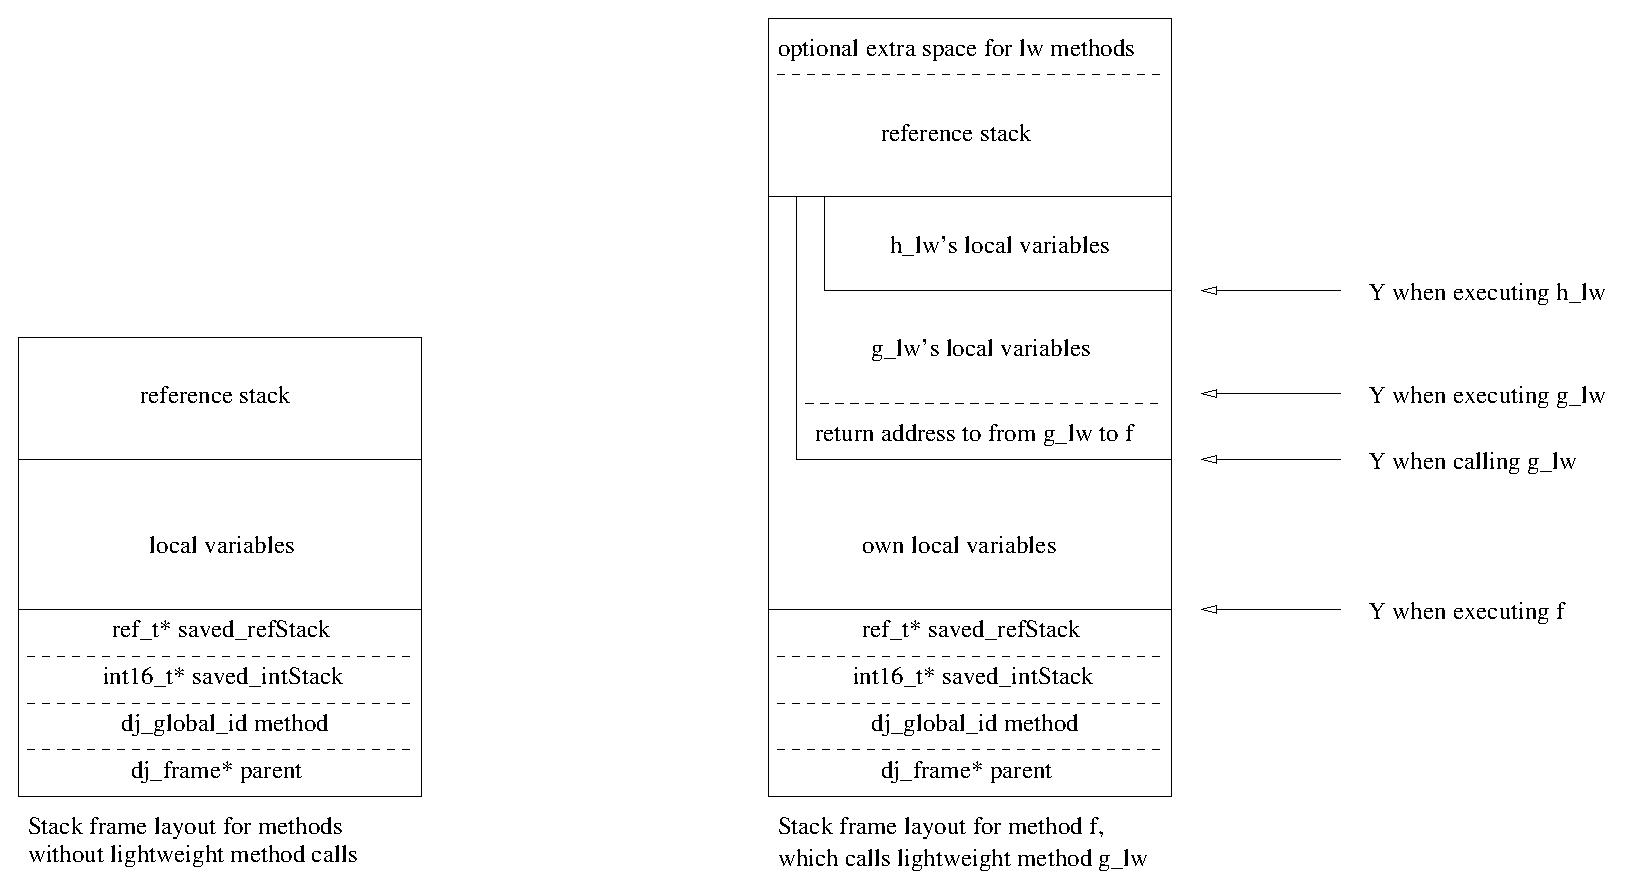
\includegraphics[width=0.95\linewidth]{stack-frame-lightweight-method.eps}
\caption{Stack frame layout for a normal method \mycode{f}, which calls lightweight method \mycode{g\_lw}, which in turn calls lightweight method \mycode{h\_lw}}
\label{fig-stack-frame-lightweight-method}
\end{figure}

An example is shown in Figure \ref{fig-stack-frame-lightweight-method}, which shows the stack frame for a normal method \mycode{f}, which calls lightweight method \mycode{g\_lw}, which in turn calls another lightweight method \mycode{h\_lw}.

The stack frame for \mycode{f} contains space for its own locals, and for the locals of the lightweight method it calls: \mycode{g\_lw}. In turn, \mycode{g\_lw}'s locals contain space for \mycode{h\_lw}'s locals, as well as a slot to store the return address back to \mycode{f}. Since \mycode{h\_lw} does not call any other methods, it just keeps its return address in registers.

When a method calls a lightweight method with local variables, it will move the Y register to point at that method's locals. From Figure \ref{fig-stack-frame-lightweight-method} it is clear it only needs to increment Y by the size of its own locals. For \mycode{f}, this will place the Y register at the beginning of \mycode{g\_lw}'s locals. Since \mycode{g\_lw} may call \mycode{h\_lw}, \mycode{g\_lw}'s prologue will first store its return address in the first local slot, moving Y forward in the process so that Y points to the first free slot.

\subsubsection{Mark loop}
Lightweight methods may use any register and do not save call-saved registers like normal methods. The only case where this would be necessary is when it is called inside a \mycode{MARKLOOP} block that uses the same register to pin a variable. In this case we save those variables back to memory before calling the lightweight method and load them after the call returns. Since lightweight methods always come before their invocation in the infusion, the VM already knows which registers it uses, and will only save and restore pinned variables if there is a conflict. Because registers for mark loop are allocated low to high, and for normal stack caching from high to low, in many cases the two may not collide.

\subsubsection{Example call}
An example of the most complex case for a lightweight call is shown in Listing \ref{lst-full-lighweight-method-call}, which shows how method \mycode{f} from Figure \ref{fig-stack-frame-lightweight-method} would call \mycode{g\_lw}, assuming \mycode{f} is in a markloop block at the time which pinned a variable R14:R15, and these registers are also used by \mycode{g\_lw}.

In the translation of the \mycode{INVOKELIGHT} instruction we see we first flush the cache to memory, and then save the value of the local short at offset 22 that was pinned to R14:R15. Finally we add 26 to the Y register to skip the caller's own local variables and point Y to the start of the space reserved for lightweight method locals.

In the method call, we first see the return address is popped off the stack into a register. Since \mycode{g\_lw} may call another lightweight method, we cannot leave it there but store it in the first local slot, incrementing Y in the process. After \mycode{g\_lw} is done, we see the reverse process to return to the caller, where we then see the Y register is restored to point to the caller's locals, and the local variable at offset 22 is loaded back into the pinned register.

\begin{listing}
\centering
\begin{minipage}[t]{0.48\textwidth}
\begin{minted}{java}
// LIGHTWEIGHT INVOCATION
INVOKELIGHT g_lw
    push r25        // Flush the cache
    push r24
    std Y+22, r14   // Save pinned value
    std Y+23, r15
    adiw Y, 26      // Move Y to g_lw's
    call &g_lw                 // locals
    sbiw Y, 26      // Restore Y
    ldd r14, Y+22   // Reload pinned value
    ldd r15, Y+23
\end{minted}
\end{minipage}\hfill
\begin{minipage}[t]{0.48\textwidth}
\centering
\begin{minted}[linenos=false]{java}
// IMPLEMENTATION OF g_lw
    pop r18     // Pop the return address
    pop r19
    st Y+, r18  // Save in 1st local,
    st Y+, r19  //  and increment Y

      .. // g_lw's body

    ld r19, -Y  // Load return address,
    ld r18, -Y  //  and decrement Y
    push r19    // Push return address
    push r18    //  onto the stack
    ret
\end{minted}
\end{minipage}
\caption{Full lightweight method call}
\label{lst-full-lighweight-method-call}
\end{listing}


\subsection{Overhead comparison}
We now compare the overhead for the various ways we can call a method in Table \ref{tbl-method-invoke-overhead-comparison}.

Manually inlining code yields the best performance, but at the cost of increasing code size if larger methods are inlined. ProGuard inlining is currently slightly expensive because of the way it always saves parameters in local variables.

Both lightweight methods options cause some overhead, although this is very little compared to a full method call. First, we need to flush the stack cache to memory to make sure the parameters are on the real stack. This this takes two \mycode{push} and eventually two corresponding \mycode{pop} instructions per word, costing 8 cycles per word. In addition, we need to clear the value tags from the stack cache, which may mean we may not be able to skip as many \mycode{LOAD} instructions after the lightweight call, but this is hard to quantify.

Next the cost of translating the \mycode{INVOKE} instruction varies depending on the situation. In the simplest case it is simply a \mycode{CALL} to the lightweight method, which together with the corresponding \mycode{RET} costs 8 cycles. The worst case is 68 cycles when the lightweight method has local variables, uses all registers, and the caller used the maximum of 7 pairs to pin variables in a \mycode{MARKLOOP} block.

After calling the method, the method prologue for lightweight methods is very simple. We just need to save the return address and restore it in the epilogue, which takes 8 cycles if we can leave it in a register, or 16 if we need to store it in a local variable slot.

For small handwritten lightweight methods this is the only cost, but for larger ones created by converting a Java method, we add \mycode{STORE} instructions to copy the parameters from the stack into local variables, as shown in Listing \ref{lst-comparison-of-handwritten-and-converted-java-lw-method}. This is similar to the only overhead incurred by ProGuard's method inlining, and costs 4 cycles per word for the \mycode{STORE}, and possibly 4 more if the corresponding \mycode{LOAD} cannot be eliminated by popped value caching.

The total overhead for a lightweight method call scales nicely with the method's complexity. For the smallest methods, the minimum is only 16 cycles, plus 8 cycles per word for the parameters. For the most complex cases this may go up to 100 to 150 cycles. But these methods must be more complex and will have a longer run time, so the relative overhead is still acceptable.

The number of cycles in Table \ref{tbl-method-invoke-overhead-comparison} is just a broad indication of the overhead. Some factors, such as the cost of clearing the value tags is hard to predict, and inlining may allow some optimisations that aren't possible with a method call. In practice the actual cost in a number of specific cases we examined varies, but is in the range we predicted.

Comparing this to a normal method call, we see the cost is much higher, and less dependent on the complexity of the method that is called. The overhead from setting up the stack frame, and the more expensive translation of the \mycode{INVOKE} instruction (see Listing \ref{lst-lightweight-stack-only}) are fixed, meaning a call will cost at least around 550 cycles, increasing to over 700 cycles for more complex methods taking many parameters.

%INVOKE COST FOR LIGHTWEIGHT METHOD:
%  8            CALL/RET
%  4            move Y
%  8 per word   saving markloop pinned registers used by lw method
%  0            pre/post invoke
%  0            setup callMethod parameters
%  
%  minimum: 8
%  maximum: 8 + 4 + 8*7 = 68
%  
%INVOKE COST FOR NORMAL METHOD:
%  8            CALL/RET
%  0            move Y
%  0            saving markloop pinned registers used by lw method
%  32+34        pre/post invoke
%  8            setup callMethod parameters
%  
%  total: 8+ = 82
\begin{table}
\caption{Approximate cycles of overhead caused by different ways of invoking a method}
\label{tbl-method-invoke-overhead-comparison}
	\centerline{
    \begin{tabular}{lccccc}
    \toprule
                                                              & Manual          & ProGuard                & Stack-only                  & Converted Java              & Normal                                              \\
                                                              & inlining        & inlining                & lightweight                 & lightweight                 & method call                                         \\
    \midrule
    \midrule
    flush the stack cache \footnote{excluding effect on future popped value cache performance because of cleared value tags}
                                                              &                 &                         & 8 per word                  & 8 per word                  & 8 per word                                          \\
    \mycode{INVOKE}                                           &                 &                         & 8 to 68                     & 8 to 68                     & \textasciitilde 82                                  \\
    create stack frame                                        &                 &                         &                             &                             & \textasciitilde 450                                 \\
    method pro-/epilogue                                      &                 &                         & 8 or 16                     & 8 or 16                     & 10 to 71                                            \\
    store and load parameters                                 &                 & 4 or 8 per word         &                             & 4 or 8 per word             & 4 or 8 per word                                     \\
    \\
    \emph{total}                                              &                 & \emph{4 or 8 per word}  & \emph{16 to 84 +}           & \emph{16 to 84 +}           & \emph{\textasciitilde 542 to \textasciitilde 603 +} \\
                                                              &                 &                         & \emph{8 per word}           & \emph{12 or 16 per word}    & \emph{12 or 16 per word}                            \\
    \bottomrule
    \end{tabular}
    }
\end{table}

\subsection{Creating lightweight methods}
We currently support two ways to create a lightweight method:
\begin{itemize}
	\item handwritten JVM bytecode
	\item converting a Java method 
\end{itemize}

\subsubsection{Handwritten JVM bytecode}
For the first option we declare the methods \mycode{native} in the Java source code, so the code calling it will compile as usual. We provide the infuser with a handwritten implementation in JVM bytecode, which the infuser will simply add to the infusion, and then process it in the same way as it processes a normal method, with one step added:

For lightweight methods, the parameters will be on the stack at the start of the method, but the infusers expects to start with an empty stack. To allow the infuser to process them like other methods, we add a dummy \mycode{LW\_PARAMETER} instruction for each parameter. This instruction is skipped when writing the binary infusion, but it tricks the infuser into thinking the parameters are being put on the stack.


\subsubsection{Converting Java methods}
This handwritten approach is useful for the smallest methods, and allows us to create bytecode that only uses the stack, which produces the most efficient code. But for more complex methods it quickly becomes very cumbersome to write the bytecode by hand.

As a second, slightly slower, but more convenient option, we developed a way to convert normal Java methods to lightweight methods by adding a \mycode{@Lightweight} annotation to it.

The infuser will scan all the methods in an infusion for this annotation. When it finds a method marked \mycode{@Lightweight}, the transformation to turn a normal JVM method into a lightweight one is simple: we first add a dummy \mycode{LW\_PARAMETER} instruction for each parameter, followed by \mycode{STORE} instructions to pop these parameters off the stack and store them in the right local variables. After this, we can use the normal body of the method and call it as a lightweight method.

Listing \ref{lst-comparison-of-handwritten-and-converted-java-lw-method} shows the difference for the \mycode{isOdd} method. We can see this approach adds some overhead in the form of a \mycode{SSTORE\_0} and a \mycode{SLOAD\_0} instruction. However, using popped value caching, only the \mycode{SSTORE\_0} will have a run-time cost. Another disadvantage of the converted method is that is has to use a local variable, which will slightly increase memory usage, but in return this approach gives us a very easy way to create lightweight methods.

\begin{listing}
 \centering
 \begin{minipage}[t]{0.32\textwidth}
  \centering
  \begin{minted}{java}
// JAVA
@Lightweight
public static boolean
          isOdd (short a)
{
  return (a & (short)1)==1;
}
  \end{minted}
 \end{minipage}\hfill
 \begin{minipage}[t]{0.29\textwidth}
  \centering
  \begin{minted}[linenos=false]{java}
// HANDWRITTEN
//              (Stack)
LW_PARAMETER    (Int)
SCONST_1        (Int,Int)
SAND            (Int)
SRETURN         ()
  \end{minted}
 \end{minipage}\hfill
 \begin{minipage}[t]{0.29\textwidth}
  \centering
  \begin{minted}[linenos=false]{java}
// CONVERTED JAVA
//              (Stack)
LW_PARAMETER    (Int)
SSTORE_0        ()
SLOAD_0         (Int)
SCONST_1        (Int,Int)
SAND            (Int)
SRETURN         ()
  \end{minted}
 \end{minipage}
 \vspace{0.5cm}

\caption{Comparison of hand written lightweight method and converted Java method}
\label{lst-comparison-of-handwritten-and-converted-java-lw-method}
\end{listing}


\subsubsection{Replacing \mycode{INVOKE}s}
The infuser does a few more transformations to the bytecode. Every method is scanned for \mycode{INVOKESTATIC} instructions that invoke a lightweight method. These are simply replaced by an \mycode{INVOKELIGHT}, and the number of extra slots for the reference stack and local variables of the current method is increased if necessary. Finally, methods are sorted so a lightweight method will be defined before it is invoked, to make sure the VM can always generate the \mycode{CALL} directly.


\subsection{Limitations and tradeoffs}
There are a few limitations to the use of lightweight methods:
\paragraph{No recursion} Since we need to be able to determine how much space to reserve in the caller's stack frame for a lightweight method's reference stack and local variables, we do not support recursion, although lightweight calls can be nested.

\paragraph{No garbage collection}
Lightweight methods reuse the caller's stack frame. This is a problem for the garbage collector, which works by inspecting each stack frame and finding the references on the stack and in local variables. If the garbage collector would be triggered while we're in a lightweight call, it would not know where to find the lightweight method's references, since the stack frame only has information for the method that owns it.

While it may be possible to relax this constraint with some effort, in most cases this is only a minor restriction. Lightweight methods are most useful for fast and frequently called methods, and operations that may trigger the garbage collector are usually expensive, so there is less to be gained from using a lightweight method in these situations.

\paragraph{Static only}
We currently do not support lightweight virtual methods, since the overhead of resolving the target of the invoke is large compared to the rest of the invoke overhead, but this is something that could be considered in future work.

\paragraph{Stack frame usage}
Finally, while many methods can be made lightweight, we should remember that a method calling a lightweight method will always reserve space for it in its locals. This space is reserved, regardless of whether the method is currently executing or not, and the more nested lightweight calls are made, the more space we need to reserve.

As an example if we have a method \mycode{f1} which may call a lightweight method with a large number of local variables, \mycode{big\_lw}, but is currently calling normal method \mycode{f2}, which may also call \mycode{big\_lw}, we will have reserved space for \mycode{big\_lw} twice, both in \mycode{f1}'s and in \mycode{f2}'s frame.


\chapter{Safety}
\label{sec-safety}
\newcounter{tcheckcnt}
\newcommand{\tcheck}[1]{\refstepcounter{tcheckcnt}T-\arabic{tcheckcnt}\label{#1}}
\newcounter{rcheckcnt}
\newcommand{\rcheck}[1]{\refstepcounter{rcheckcnt}R-\arabic{rcheckcnt}\label{#1}}

\makeatletter
\renewcommand\p@tcheckcnt{T-\arabic{tcheckcnt}\expandafter\@gobble}
\renewcommand\p@rcheckcnt{R-\arabic{rcheckcnt}\expandafter\@gobble}
\makeatother

\begin{table*}
\centering
\caption{List of safety checks}
\label{tbl-safety-checks}
\begin{tabular}{lp{0.9\linewidth}}
\toprule
 & Translation-time checks \\

\tcheck{chk-method-header-is-sane}
	& For each method header, the number of own local variable slots <= the number of total variable slots, the number of (int/ref) arguments <= the number of (int/ref) variables, static methods are not abstract. \\

\tcheck{chk-return-or-goto-at-end-of-method}
	& The last instruction of each method is a \mycode{RETURN} or \mycode{GOTO}. \\

\tcheck{chk-brtarget-exists}
	& Branch instructions branch to an index < the number of \mycode{BRTARGET}s announced in the method header. \\

\tcheck{chk-all-brtargets-found}
	& At the end of each method, we have seen the exact number of \mycode{BRTARGET} instructions announced in the method header. \\

\tcheck{chk-invokelight-target-found}
	& The target for an \mycode{INVOKELIGHT} call is already translated, so the target address is known. \\

\tcheck{chk-invokestatic-target-header-found}
	& The target method header for an \mycode{INVOKESTATIC}/\mycode{INVOKESPECIAL} exists. \\

\tcheck{chk-stack-is-empty-after-return}
	& After popping the return value, the stack is empty. \\

\tcheck{chk-sufficient-locals-at-invokelight}
	& For each \mycode{INVOKELIGHT}, the total number of slots - the number of own variable slots for the caller >= the total variable slots for the callee. \\

\tcheck{chk-sufficient-stack-space-at-invokelight}
	& At the point of an \mycode{INVOKELIGHT} instruction, the max stack of the caller >= the current stack depth - the number of arguments to the callee + the max stack of the callee. \\

\tcheck{chk-stack-is-empty-at-branches}
	& The stack is empty at branches and branch targets. \\

\tcheck{chk-no-operandstack-underflow}
	& Before each instruction, the stack depth >= the number of elements to be consumed by the instruction. \\

\tcheck{chk-no-operandstack-overflow}
	& After each instruction, the stack depth <= the max stack depth announced in the header. \\

\tcheck{chk-local-variable-slot-exists}
	& The index of the local variable < the number of own variable slots for the current method. \\

\tcheck{chk-static-variable-infusion-exists}
	& The target infusion of a static variable exists. \\

\tcheck{chk-static-variable-slot-exists}
	& The index of the static variable < the number of static variable slots for the target infusion. \\

\midrule
& Run-time checks \\

\rcheck{chk-invokevirtual-target-found}
	& The target implementation for an \mycode{INVOKEVIRTUAL}/\mycode{INVOKEINTERFACE} is found. \\

\rcheck{chk-no-nativestack-overflow}
	& Whenever a new stack frame is allocated the frame+max stack depth+some safety margin > the end of the heap. \\

\rcheck{chk-invokevirtual-stack-effects-match}
	& The target implementation for an \mycode{INVOKEVIRTUAL}/\mycode{INVOKEINTERFACE} matches the stack effects used to verify the caller's stack at translation time. \\

\rcheck{chk-memory-access-within-heap}
	& The target address of an array element or object field is within the heap. \\

\bottomrule
\end{tabular}
\end{table*}

The second goal of this dissertation is to develop a VM that offers a 'safe' execution environment, and to compare the cost of doing so in a VM to existing native code approaches.

A safe execution environment is one that guarantees an application cannot harm the system it's running on or other applications running on the same system. Specifically, an application cannot:
\begin{enumerate}
	\item write to memory outside the areas assigned to it,
	\item execute code it does not have permission for, or
	\item retain control of the CPU indefinitely
\end{enumerate}

Given the first two, the last guarantee is easy to implement: the VM can simply set a timer to trap back to the VM after a certain amount of time. As long as the other guarantees hold, the application will not be able to disable the timer without the VM's permission.

To guard against programming errors as well as malicious attacks, we focus on the second type of approaches shown in Figure \ref{fig-safe-compilation-process}, where the node does not rely on the host to guarantee safety, but can do so independent of the code it receives.

As discussed in Chapter 3, most generic sensor nodes VMs do not consider safety, with the exception of SensorScheme \cite{Evers:2010ur}. This is unfortunate because the complexity of reducing the necessary run-time checks noted by native code systems like Harbor \cite{Kumar:2007ge}, is much lower when using a virtual machine. Compared to native CPU instruction sets, the JVM instruction set is relatively simple and restricted, and easier to reason about. As we will see, many checks can be done at translation time, reducing the need for run-time checks and the corresponding overhead.

For an interpreter, the VM is always in control, which makes it is easy to guarantee safety, but interpreters come at the cost of a one to two orders of magnitude performance penalty. CapeVM is an Ahead-of-Time compiler, which translates JVM bytecode to native code at load-time to reduce interpretation overhead. This means the application is executing native code for most of the time, only occassionaly calling functions in the VM to handle more complex operations. However, all of this code is generated by the VM, which means it can perform checks at translation time to ensure the code it generates is safe. Run-time checks are only inserted when it is impossible to guarantee safety at translation time.

To guarantee safety we first make the guarantees more concrete and specific to CapeVM:

\begin{itemize}
	\item \emph{control flow safety}: the VM is always executing either
		\begin{itemize}
			\item a translated JVM instruction from the top, so code cannot jump to a point half-way a generated instruction with undefined results, or
			\item code in the VM itself, as a result of either a call to the VM from a translated JVM instruction, or returning from the main method
		\end{itemize}
	\item \emph{memory safety}: any write to memory done by the application is to a legal location: either
		\begin{itemize}
			\item memory reserved for the operand stack, or
			\item a valid local or static variable, or
			\item the area of the heap assigned to the application
		\end{itemize}
\end{itemize}

Both depend on the other: memory safety is assumed when discussing control flow safety and vice versa. For each, we will examine each bytecode instruction to determine its effect, and what additional checks are necessary to guarantee safety.

The resulting checks are listed in Table \ref{tbl-safety-checks}. Compared to the checks specified in Section 4.10 of the Java Virtual Machine Specification \cite{Lindholm:2017vu}, the checks are different in two ways, they are specific to our VM's implementation, and since the goal is to ensure safety, CapeVM's checks are less restrictive than the JVM specification. For example, they allow writing to a private field from outside the class since this, while incorrect, is not a safety violation. 

Each method in our VM has a small \emph{method header} defining properties such as the maximum stack size, number of local variables, return type, etc. Since the VM uses this header to determine the required size of the stack frame and the effects of a method call on the operand stack, many of the necessary checks are to ensure the actual bytecode follows the contract established in the method header. When the node receives new bytecode, it receives the headers for all methods first, followed by the implementations, so the contracts for all methods are known when we start translating the byte code.

The first check is a basic sanity check on the data in the method headers (\ref{chk-method-header-is-sane}). For example, since each parameter becomes a local variable, the number of local variable slots must be at least as high as the number of parameter, and the total number of slots must be at least as high as the method's own local variable slots, while the rest may be used for lightweight methods.

\section{Control flow safety}
We guarantee control flow safety by considering the effect of each possible JVM instruction, and showing they either flow into the start of a legal next instruction, or return control back to the VM. Instructions are grouped into four categories, shown in Table \ref{tbl-control-flow-instructions}. Most instructions don't affect the control flow. The ones that do are: branches, method invocations, and returns. The state is correct at the start of the programme, since the VM will start it by jumping to the beginning of the first instruction in the main method. We will show the state will be correct after each following instruction by looking at these four categories.

\begin{table}
\caption{Instructions affecting control flow}
\label{tbl-control-flow-instructions}
    \begin{tabular}{ll}
    \toprule
    Type              & Effect on control flow \\
    \midrule
    \midrule
    Branches          & Jump to a location within the method \\
    \mycode{INVOKE}s  & Call a method, either through the VM or directly \\
    \mycode{RETURN}s  & Return to the address at the top of the stack \\
    Others            & Fall through to the next JVM instruction \\
    \bottomrule
    \end{tabular}
\end{table}

\subsection{Simple instructions}
Starting with the last category: most instructions such as math operations, loads and stores, are translated to a sequence of native instructions that will be executed top to bottom. In some cases this may call to a VM or libc function to perform some complex operation, but these calls all eventually return to the current instruction.

For this category, the generated code will flow naturally into the next generated instruction, which is safe as long as there \emph{is} a next instruction. This produces the second translation-time check, \ref{chk-return-or-goto-at-end-of-method}: the last instruction in a method should be a \mycode{RETURN} or \mycode{GOTO} to prevent control from flowing into undefined territory after the method body.

\subsection{Branch instructions}
In CapeVM bytecode, which is a modified form of standard JVM bytecode, branches don't target an offset as in normal JVM bytecode, but a branch target ID. These targets are marked with a \mycode{BRTARGET} instruction, which doesn't emit any code, but causes the AOT compiler to collect the address in a temporary table during translation. Once the whole method is translated, this temporary table is used to patch the correct target address into the branch instructions to handle forward branches.

Each method announces the number of branch targets that will be used in the method header. To ensure each taken branch will branch to a legal instruction within the method, two checks are needed: the target ID of each branch must be lower than number of branch targets announced in the method header to make sure it refers to an entry in the temporary table (\ref{chk-brtarget-exists}), and at the end of the method the number of \mycode{BRTARGET} instructions encountered must be equal to the number announced in the header so all table entries will point to a valid address in the method (\ref{chk-all-brtargets-found}).

\subsection{Invoke instructions}
There are three kinds of method invocations.

For lightweight method calls, the implementation of the target method is required to come before any method invoking it, to ensure the address of target is known at translation time and we can directly generate a \mycode{CALL} to the method. Ensuring this calls to a correct address is therefore trivial: at any \mycode{INVOKELIGHT}, code for the target method must already have been generated (\ref{chk-invokelight-target-found}).

For static calls (\mycode{INVOKESTATIC} and \mycode{INVOKESPECIAL}) the target method is known at translation time, but it may not have been translated yet if the implementation follows later in the infusion. For these instructions, a \mycode{CALL} to the VM's \mycode{callMethod} function is generated, passing the id of the target method as a parameter. At run time this id will be used as an index in the method table. Because the VM receives all the method headers before translating their implementations, it can check at translation time that the method id is known (\ref{chk-invokestatic-target-header-found}). Since the VM won't start an application before the implementation for all methods is translated, this guarantees that \mycode{callMethod} will be able to find the correct target at run time.

Finally, for \mycode{INVOKEVIRTUAL} and \mycode{INVOKEINTERFACE}, the target is not known at translation time, since this depends on the object the method is invoked on, which will not be known until run time. Therefore a run-time check is needed to verify the method can be found (\ref{chk-invokevirtual-target-found}), but since the method already needs to be resolved to make the call, this doesn't add any extra overhead.

\subsection{Return instructions}
\label{sec-control-flow-safety-return-instructions}
Finally, return instructions pop the return value from the stack, and then do a native \mycode{RET} instruction to return, either directly to the AOT compiled code of the caller for lightweight method calls, or to the VM's \mycode{callMethod} function.

The \mycode{RET} instruction takes the return address from the native stack, which is also used to store the JVM's integer operand stack. This means the integer operand stack needs to be empty at return instructions (\ref{chk-stack-is-empty-after-return}) to ensure the correct address will be at the top of the native stack. Memory safety then guarantees the application could not have corrupted it. Without this check, malicious code could leave an integer on the stack and use the return instruction to jump to an arbitrary location.

A second way the return address could be corrupted is if the native stack overflows into the JVM heap. In CapeVM the heap is a fixed sized block that sits above other global variables, and the native stack grows down towards it. If the native stack grows into the area reserved for the heap, a return address may be corrupted.

To prevent this a run-time check is added to non-lightweight invokes, that checks the stack frame for the called method, plus it's maximum integer stack size, does not grow into the heap (\ref{chk-no-nativestack-overflow}). Lightweight calls do not add to the stack, since space for their local variables, stack, and return address was already allocated in the caller's frame.

While running, a method may make calls to the VM or libc functions, causing the stack to grow further. Since the maximum stack growth for such calls is fixed, a certain safety margin is added between the stack and heap. A similar gap of 128 bytes between the stack and kernel heap is reserved by \emph{t-kernel} \cite{Gu:2005un}, although it is not clear from the paper whether this is for the same reason.

\section{Memory safety}

\begin{figure}
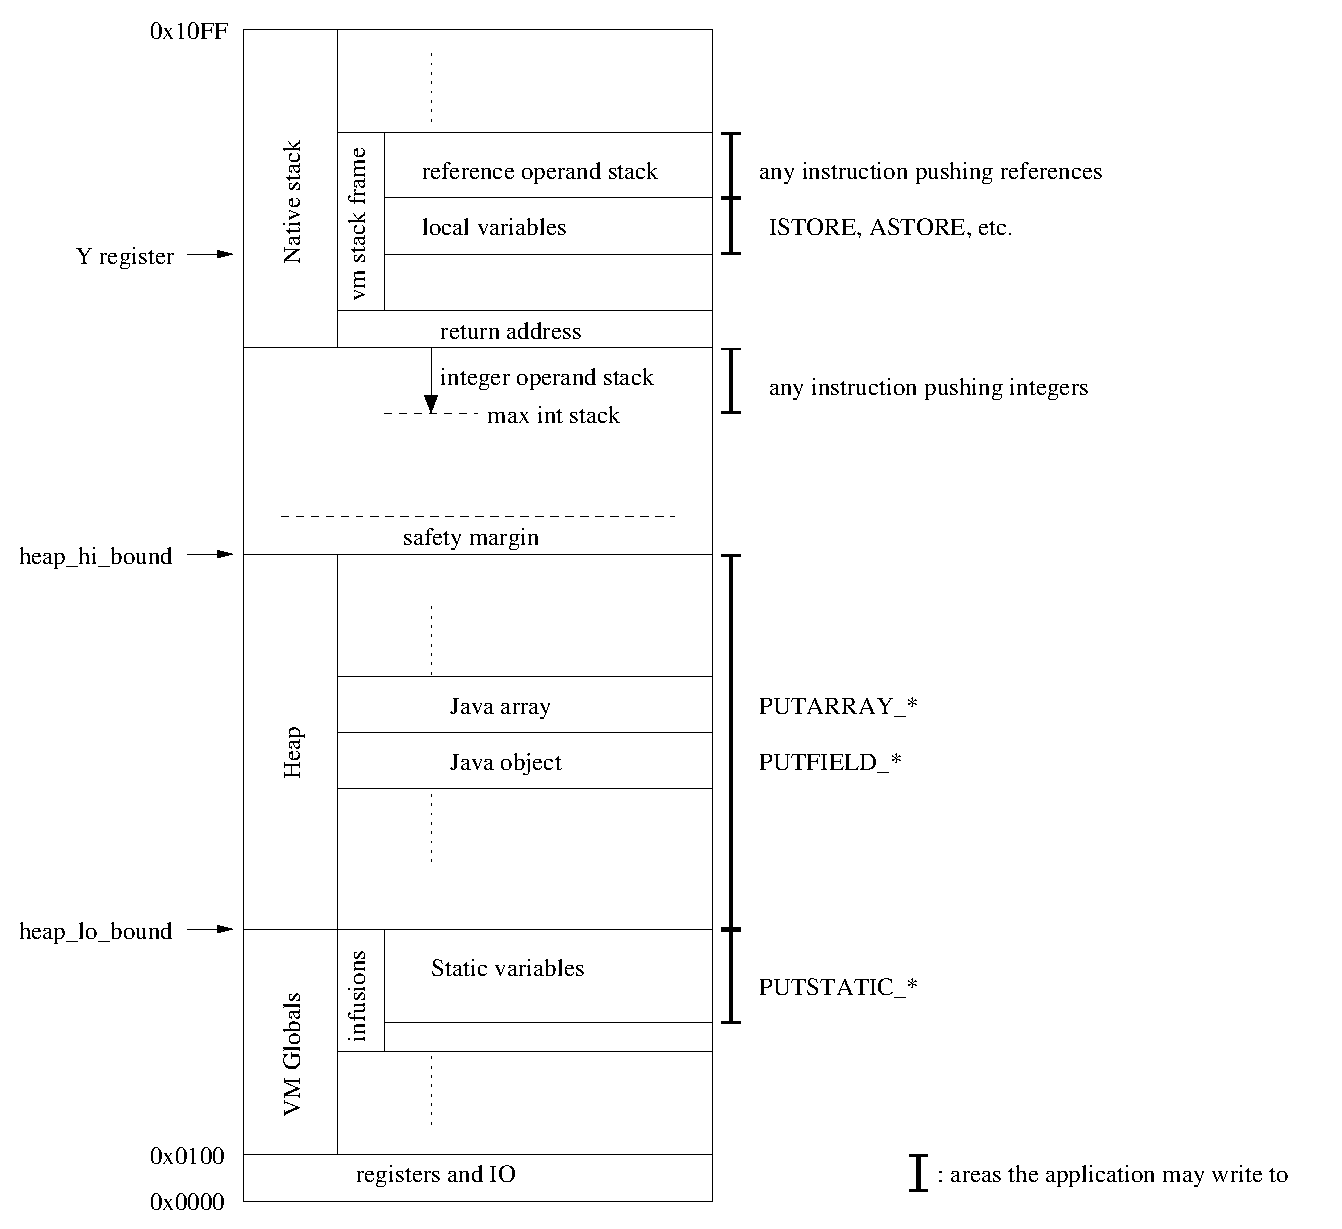
\includegraphics[width=\linewidth]{memlayout.eps}
\caption{Global memory layout and the areas accessible to the application}
\label{fig-memlayout}
\end{figure}

Figure \ref{fig-memlayout} shows the global layout of the VM's memory. At the bottom are the internal state of by the VM, stored in a number of global variables, and a block with static variables for each infusion. The infusion blocks are actually allocated at the bottom of the heap at startup, after which this part of the heap is separated from the range the application may use to protect them from bad heap writes. This is followed by the application heap, which contains Java objects and arrays.

The native stack grows down in memory towards the heap. This contains a mix of native stack frames for internal VM functions, the application's JVM stack frames containing space for local variables and reference operand stack, and the integer operand stack which grows down directly on top of the native stack.

The VM's private data and the application data are mixed in the node's memory. The application is only allowed to write to the areas indicated with bars to the right. Any write outside of these designated areas may corrupt the VM's internal state, and needs to be prevented by our safety checks.

Having ensured control flow safety, we can now rely on the fact that we will always execute complete JVM instructions, and the application cannot skip past an inserted run-time check by jumping to the middle of a generated instruction. This means we can demonstrate memory safety by considering each how complete JVM instructions write to memory, and showing they are all either guaranteed to write to a correct address, or checked at run time. Again, instructions are grouped with respect to their memory writes, as shown in Table \ref{tbl-memory-write-instructions}.

\begin{table}
\caption{Instructions writing to memory}
\label{tbl-memory-write-instructions}
    \begin{tabular}{ll}
    \toprule
    Type                                 & Writes to \\
    \midrule
    \midrule
    Any instruction pushing to the stack & The reference or integer stack \\
    \mycode{STORE}s                      & A local variable in the current method's stack frame \\
    \mycode{PUTSTATIC}s                  & A static variable in an infusion \\
    \mycode{PUTARRAY}s                   & An array on the heap \\
    \mycode{PUTFIELD}s                   & An object on the heap \\
    \bottomrule
    \end{tabular}
\end{table}


\subsection{The operand stack}
The VM will reserve space for the operand stacks (all of this section applies equally to the integer and reference stack), based on the information in the method headers, so it needs to make sure the actual stack depth neither underflows, or exceeds the maximum announced in the header.

For normal methods, the VM creates a stack frame based on the method header, so at translation time we know exactly how much space will be available at run time. Lightweight methods don't create their own stack frame, but depend on the caller's stack frame. Whenever an \mycode{INVOKELIGHT} instruction is translated, the VM needs to verify the stack frame of the current method has reserved enough free space for the invoked lightweight method's stack (\ref{chk-sufficient-locals-at-invokelight}). To do this, the method header contains both the total number of slots to reserve, and the number the method will use for it's own slots. Any remaining slots are available to lightweight methods.

The effect of each instruction on the stack is known at translation time, so the stack depth can be verified in a single top to bottom pass. The VM maintains two counters indicating how many values are on the integer and reference stacks, and updating these counters for each instruction's stack effects, as the instructions are being translated. For normal methods both counters are initialised to 0, since they start with empty stacks. Lightweight methods start with their parameters on the stack, so for these the counters are initialised according to the number of arguments announced in the method header.

For each translated instruction, the VM checks there are enough values on the stack to consume its operands (\ref{chk-no-operandstack-underflow}), and that maximum stack depth announced in the header is not exceeded after pushing it's results (\ref{chk-no-operandstack-overflow}).

Most bytecode instructions have a fixed effect on the stack, for example \mycode{IADD} will always consume two 32-bit ints and push another. We encode this in a simple table. Method calls, discussed below, require some more work to determine the stack effects. 

\paragraph{Branches}
The \mycode{BRTARGET} instruction poses a problem for this single pass approach since they can be reached from multiple locations, so the stack depth when entering this instruction is unknown.

The simplest way to solve this is to require the stack to be empty at all branches. As mentioned in \ref{sec-optimisations-simple-stack-caching}, this is already the case for most code generated by \mycode{javac}.

Alternatively, the expected stack state at each branch target could be included in the method header, which would allow the VM to check the state matches at each branch and branch target. However, this is more complex and in practice the overhead for requiring an empty operand stack at branches is minimal: in our entire Java codebase only a few small modifications were necessary, which a future combined optimising compiler and infuser could do automatically.

Thus, the VM only verifies the stack is empty at branches and branch targets (\ref{chk-stack-is-empty-at-branches}).

\paragraph{Invoke instructions}
The \mycode{INVOKESTATIC}, \mycode{INVOKESPECIAL}, and \mycode{INVOKELIGHT} instructions all contain the id of the method that will be invoked. Since all method headers are available at translation time, and they contain the number of arguments and return type, it is easy to determine the stack effects of these invoke instructions.
 
For \mycode{INVOKEVIRTUAL} and \mycode{INVOKEINTERFACE} however, the actual method that will be called depends on the object on the stack at run time. For these, the expected stack effect is determined based on the first implementation that matches the call. For valid code all implementations should have the same signature, and thus the same effect on the stack, but malicious code could try to send an implementation in a subclass that has different stack effects. Therefore, a run-time check (\ref{chk-invokevirtual-stack-effects-match}) is added that will verify the method that is called at run time, has the same stack effects as the one used to verify the stack at translation time.

\paragraph{Return instructions}
Note that \mycode{RETURN} instructions don't need any special care. The stack depth in the method is verified using the instruction found in the bytecode. It's possible for a method to break the contract established in the method header, for example by using \mycode{RETURN} instead of \mycode{IRETURN} in a method that should return an int. However, this is still safe as long as the stack is empty after the return instruction, as checked by \ref{chk-stack-is-empty-after-return}.

Because the return value is passed in registers to the calling method, the result of using an incorrect return instruction is that either the return value is discarded, or whatever happens to be in the registers is used as a return value, which may corrupt the application's own state, but not the VM's.

\subsection{\mycode{STORE}}
Local variables are accessed as an offset from the \mycode{Y} register, which is under control of the VM and points to the start of the local variables, as shown in Figure \ref{fig-memlayout}. As for the operand stack, the method header contains the number of variable slots that will be allocated in a normal method method's stack frame. For lightweight methods, the VM checks all \mycode{INVOKELIGHT} instructions to verify the caller has reserved enough local variable slots for any lightweight method it may call (\ref{chk-sufficient-stack-space-at-invokelight}), so the number of slots specified in a lightweight method's header is guaranteed to be available at run time.

Local variables are written to using the \mycode{STORE} instructions. Each \mycode{STORE} instruction contains the index of the local variable slot to write to, so the VM only needs to check at translation time that the index of the local is within the range announced in the method header, to guarantee it writes to a valid location (\ref{chk-local-variable-slot-exists}).

\subsection{\mycode{PUTSTATIC}}
Static variables are allocated globally at the start of the application based on number of static variables in the \emph{infusion} header. The \mycode{PUTSTATIC} instruction contains a reference to an infusion, and the index of the target static variable slot. At translation time, the VM checks the referenced infusion exists (\ref{chk-static-variable-infusion-exists}), and the index is within the legal range (\ref{chk-static-variable-slot-exists}) for that infusion.

\subsection{\mycode{PUTFIELD} and \mycode{PUTARRAY}}
\label{sec-safety-heap-access}

\begin{listing}
	\centering
 	\begin{minted}{c-objdump}
    heapcheck:
        lds  r0, heap_lo_bound
        cp   ZL, r0
        lds  r0, heap_lo_bound + 1
        cpc  ZH, r0
        brlo illegal_access_handler:
        lds  r0, heap_hi_bound
        cp   r0, ZL
        lds  r0, heap_hi_bound + 1
        cpc  r0, ZH
        brlo illegal_access_handler:
        ret
	\end{minted}
	\caption{Heap bounds check}
	\label{lst-heap-bounds-check}
\end{listing}


%\begin{listing}
%	\centering
% 	\begin{minted}{c-objdump}
%    heapcheck:                               cycles   bytes
%        lds  r0, heap_lo_bound               2        4
%        cp   ZL, r0                          1        2
%        lds  r0, heap_lo_bound + 1           2        4
%        cpc  ZH, r0                          1        2
%        brlo illegal_access_handler:         1        2
%        lds  r0, heap_hi_bound               2        4
%        cp   r0, ZL                          1        2
%        lds  r0, heap_hi_bound + 1           2        4
%        cpc  r0, ZH                          1        2
%        brlo illegal_access_handler:         1        2
%        ret                                  4        2
%	\end{minted}
%	\caption{Heap bounds check}
%	\label{lst-heap-bounds-check}
%\end{listing}

The final type of memory access is to the heap. The various \mycode{NEW} instructions used to create arrays and objects are safe since they are fully implemented in the VM, which only allocates new objects at a valid heap location. Writes to heap memory happen using the \mycode{PUTFIELD} and \mycode{PUTARRAY} instructions, which write to object fields and array elements respectively. 

These instructions both work on an object reference, so a null reference bug could easily trick the VM to write to the lowest addresses. Since in the AVR, the lowest 32 bytes of the address space are mapped to the CPU's general purpose registers, this can cause very hard to diagnose bugs. Similarly, using a high out-of-bounds index into an array, malicious code could gain access to the native stack and, for instance, corrupt return addresses.

In some cases it may be possible to verify of these operations at translation time, but this is hard without extensive analysis that would be too expensive for a sensor node. Therefore a run-time check is added when translating these instructions, which checks the target address is within the heap just before doing the final memory access (\ref{chk-memory-access-within-heap}).

The VM stores the bounds of the heap in two variables: \mycode{heap\_lo\_bound} and \mycode{heap\_hi\_bound} as shown in Figure \ref{fig-memlayout}. Each heap access instruction calculates the address to write in the AVR's \mycode{Z} register. Just before the actual write to the heap, we insert al \mycode{CALL} to the \mycode{heapcheck} function shown in Listing \ref{lst-heap-bounds-check}. This function checks the address in \mycode{Z} is within these bounds. If not, it jumps to the \mycode{illegal\_access\_handler}, allowing the VM to terminate the application. This check adds 22 cycles overhead for each array or object write, and 4 bytes code size overhead for the \mycode{CALL} instruction.

The actual write to the heap is often done by an offset from \mycode{Z} using the AVR's \mycode{STD}, or 'store indirect with displacement' instruction, that allows us to write to a fixed offset of at most 63 bytes from \mycode{Z}. For example, to write to object fields, who's offset within the object is know at translation time, we simply load the object's address into \mycode{Z} and use \mycode{STD} to write to the correct offset.

This means the write target an address of at most 63 bytes above the end of the heap. One way to avoid this is avoid the \mycode{STD} instruction, and instead use the \mycode{ADIW} instruction to first add the offset to \mycode{Z} and then use the normal \mycode{ST} instruction to store without displacement. However, this would add 2 bytes and 2 cycles for instruction. Instead we reuse the same small safety margin mentioned in Section \ref{sec-control-flow-safety-return-instructions} for check \ref{chk-no-nativestack-overflow}. This is safe because we never write to a heap object and execute a function in the VM or libc at the same time.

\paragraph{Alternative solutions}
We considered several alternative implementations for \mycode{heapcheck}. Since the \mycode{CALL} and \mycode{RET} instructions are expensive, 7 cycles can be saved by inlining in the check instead of calling it. However, this increases the code size overhead from 4 bytes to over 30 bytes, which we consider too high.

If we align the top and bottom boundaries of the heap at 256 bytes, this eliminates the need to check the lower byte of the \mycode{Z} register, \mycode{ZL}. This saves 6 of the 22 cycles, but wastes RAM since some bytes below and above the heap would have to remain unused. Since RAM is such a scarce resource and the performance gain is limited, we decided against this.

Finally, 8 cycles can be saved by keeping the bounds in registers instead of memory, which removes the need for the \mycode{LDS} instructions. However this reduces the performance of the stack cache since these registers would not be available for stack caching. Which of these affects performance more depends on the code being run. We evaluate the difference in Section \ref{sec-evaluation-run-time-cost}. Since the option to have the bounds in registers is more complex to implement, thus increasing VM size, we choose to keep the bounds in registers.


\section{Hardware acceleration}
Sensor node CPUs do not have features such as memory management units (MMUs) and privileged-mode execution used in desktop CPUs. While the added complexity for these cannot be justified in a market driven by extreme pressure to minimise chip cost and area, some more lightweight support from the hardware could significantly reduce the cost of providing safe execution environments, with or without a VM.

In this section we consider two possible extensions to the CPU that can be implemented at little cost in terms of chip surface area, and we believe to be generic enough to justify their inclusion in these CPUs.

The two most expensive checks are \ref{chk-no-nativestack-overflow} and \ref{chk-memory-access-within-heap}. The last is the cause of most of the run-time overhead, and both require us to keep a safety margin in between the heap and stack. While this margin is small, RAM memory is a scarce resource we would prefer not to waste.

We propose two checks to be added to the CPU, causing it to trap to a fixed error handler when the check fails to allow the node to terminate the faulty programme.

\subsection{Stack overflow protection}
To protect against stack overflow, we propose extending the CPU with a stack bound register. The CPU compares the stack pointer to this stack bound whenever it is modified, either by a direct write or implicitly by a \mycode{PUSH} instruction. If the stack pointer drops below the stack bound, the CPU traps to the error handler.

In our VM, the stack bound register would be set to the value of \mycode{heap\_hi\_bound}, which eliminates the need for \ref{chk-no-nativestack-overflow}.

For other embedded code this is also a useful safety measure, since the low amount of RAM makes stack overflows a real risk in any application, which can lead to unpredictable behaviour and hard to diagnose bugs.

\subsection{Heap write protection}
To eliminate the need to call \mycode{heapcheck} before each write, we propose adding two more registers containing the lower and upper bounds of the area the application is legally allowed to write to. The CPU then checks that writes to memory fall within these bounds, and otherwise traps to the error handler.

The question then is which writes should be checked, since the VM itself, or any other runtime hosting a sandboxed application, should still be able to write to any location, and CPU is not aware of which instructions are part of the VM or part of the application. Several options may be considered:

\subsubsection{Checked store instructions}
The ATmega's instruction set contains several blocks of unused opcodes \cite{Atmel:AVRInstructionSetManual}. Indirect stores can be done using an address in three register pairs: \mycode{X}, \mycode{Y}, or \mycode{Z}. There is enough space to add checked versions of the 'store indirect with displacement' instruction through one of these register pairs. When a store happens using these checked versions, the CPU does the bounds checks, while stores using the unchecked versions can still write to anywhere in memory.

The VM can then use these checked versions when generating code for \mycode{PUTFIELD} and \mycode{PUTARRAY} to implement \ref{chk-memory-access-within-heap} at no run-time cost, and use the unchecked versions for stores that are known to be safe at translation time, such as \mycode{PUTSTATIC}.

Native code approaches like Harbor, which normally verifies writes to memory are guarded by a check similar to ours, can now allow direct stores as well, as long as the checked store instructions are used, and avoid the run-time overhead for these cases.

However, using the majority of the currently unused opcodes for this feature may be too high a price to pay.

\subsubsection{Protected mode}
Alternatively, a status bit may be added to the CPU to indicate a protected mode, and only two instructions to set or clear this protected mode bit. When the CPU is in protected mode, all stores are required to fall within the heap bounds, while in unprotected mode the entire address range is accessible.

Instead emitting a call to \mycode{heapcheck}, our VM may now protect the stores for \mycode{PUTFIELD} and \mycode{PUTARRAY} by setting and unsetting the protected mode bit. Since these instructions should only take a single cycle, this would reduce the cost of such checks from 22 to just 2 cycles. Similar to the previous case, native code approaches can also benefit by allowing both writes to memory through the existing guard methods, as well as direct stores preceded by the instruction to turn on protected mode.

\chapter{Evaluation}
\label{sec-evaluation}
This dissertation presents a number of techniques to improve the performance of sensor node virtual machines and make them safe, while staying within the constraints set out in Section \ref{sec-CapeVM-goals}. This chapter evaluates to what extent CapeVM meets these goals by measuring its performance and code size overhead for a number of different benchmarks.

First, Section \ref{sec-evaluation-benchmarks} describes our experimental setup, the benchmarks used, and how the source code for these benchmarks was obtained.

Next, Section \ref{sec-evaluation-coremark} uses the largest benchmark to examine the effect of the lack of optimisations done by the standard \mycode{javac} compiler, and the manual optimisations performed on the Java source.

Sections \ref{sec-evaluation-aot-translation-performance}, \ref{sec-evaluation-aot-translation-code-size} and \ref{sec-evaluation-benchmark-details} evaluate the result of the optimisations to the AOT translation process on performance and code size.

Sections \ref{sec-evaluation-const-array} and \ref{sec-evaluation-method-invocation} focus on two specific optimisations: adding support for constant arrays and lightweight method calls.

The cost of adding safety checks is examined in Section \ref{sec-evaluation-safety}, which also compares CapeVM's overhead to existing native code systems that provide safety.

Platform independence is one of the main reasons to use a VM. While CapeVM was only implemented for the ATmega128, Section \ref{sec-evaluation-other-platforms} presents measurements that give an indication of the expected performance on other common sensor node platforms.

Finally, in Section \ref{sec-evaluation-limitations} we discuss the limitations and cost of using a VM, and describe some known hard cases which CapeVM currently does not handle as well.

\section{Benchmarks}
In this section we will briefly describe how the source code for each benchmark was obtained, and describe any relevant details in their implementation.

\subsection{MoteTrack}
\label{sec-evaluation-benchmark-implementation-motetrack}


\section{CoreMark}
\label{sec-evaluation-coremark}

First, we will examine the CoreMark benchmark. CoreMark was developed by the Embedded Microprocessor Benchmark Consortium as a general benchmark for embedded CPUs. It consists of three main parts:
\begin{itemize}
  \item matrix multiplication
  \item a state machine
  \item linked list processing
\end{itemize}

As mentioned before, we kept the Java versions as close to the original C code as possible. The other benchmarks are all relatively simple, and porting them to Java is straightforward. CoreMark is a much more comprehensive benchmark, and the more complex code exposes some challenges when using Java on embedded devices.

The biggest complication is that CoreMark makes extensive use of pointers, which do not exist in Java. In cases where a pointer to a simple variable is passed to a function, we simply wrap it in a wrapper object. A more complicated case is the \mycode{core\_list\_mergesort} function, which takes a function pointer parameter \mycode{cmp} used to compare list elements. Two different implementations exists, \mycode{cmp\_idx} and \mycode{cmp\_complex}. Here we choose the most canonical way to do this in Java, which is to define an interface and pass an object with the right to implementation \mycode{core\_list\_mergesort}.

Finally, the C version of the linked list benchmark takes a block of memory and constructs a linked list inside it by and treating it as \mycode{list\_head} and \mycode{list\_data} structs, shown in Listing \ref{lst-coremark-list-data-structures}. One way to mimic this as closely as possible is to use an array of shorts of equal size to the memory block used in the C version, and use indexes into this array instead of pointers. However this leads to quite messy code.

Instead we choose the more natural Java approach and define two classes to match the structs in C and create instances of these to initialise the list. This is also the faster option because accessing fields is faster than array access. The trade-off is memory consumption, since each object has its own heap header.

\begin{listing}[H]
 \centering
 \begin{minipage}[t]{0.45\textwidth}
  \centering
  \begin{minted}[fontsize=\scriptsize]{c}
typedef struct list_data_s {
    ee_s16 data16;
    ee_s16 idx;
} list_data;

typedef struct list_head_s {
    struct list_head_s *next;
    struct list_data_s *info;
} list_head;
  \end{minted}
 \end{minipage}\hfill
 \begin{minipage}[t]{0.45\textwidth}
  \centering
  \begin{minted}[fontsize=\scriptsize]{java}
public static final class ListData {
    public short data16;
    public short idx;
    }

public static final class ListHead {
    ListHead next;
    ListData info;
}
  \end{minted}
 \end{minipage}
\caption{C and Java version of the CoreMark list data structures}
\label{lst-coremark-list-data-structures}
\end{listing}

\subsection{Manual optimisations}
\label{sec-evaluation-manual-optimisations}
After translating the C to Java code, we only do 'fair' manual optimisations that we believe a future optimising infuser could easily do automatically. Since CoreMark is our most comprehensive benchmark, we use it to evaluate the effect of these manual optimisations.

\begin{table*}[]
\begin{minipage}{\textwidth} 
\centering
\caption{Effect of manual source optimisation on the CoreMark benchmark}
\label{tbl-coremark-manual-optimisation}
\small
\begin{tabular}{lrrrrrrrr}
\toprule
                                                                     & \multicolumn{2}{l}{list}     & \multicolumn{2}{l}{matrix}     &  \multicolumn{2}{l}{state}       & \multicolumn{2}{l}{total}     \\
                                                                     & \tiny time \footnote{in millions of cycles} & \tiny vs nat. C & \tiny time  & \tiny vs nat. C& \tiny time  & \tiny vs nat. C& \tiny time  & \tiny vs nat. C \\

                                                                     
\hline
native C                                                             &        17.9 &                &          49.8 &                &        18.4   &                  &         86.0 &                \\
baseline                                                             &       122.0 &       (+583\%) &         367.8 &       (+639\%) &       293.7   &       (+1496\%)  &        783.5 &       (+811\%) \\
optimised, using original source                                     &        52.6 &       (+195\%) &         239.1 &       (+380\%) &        82.8   &        (+350\%)  &        374.4 &       (+335\%) \\
% ORIGINAL ABSOLUTE DATA
% \makebox[5mm]{} \tiny manually inline small methods                & \tiny  52.2 & \tiny (+192\%) & \tiny   201.9 & \tiny (+305\%) & \tiny  65.8   & \tiny  (+258\%)  & \tiny  319.9 & \tiny (+272\%) \\
% \makebox[5mm]{} \tiny use short array index variables              & \tiny  59.0 & \tiny (+231\%) & \tiny    92.5 & \tiny  (+86\%) & \tiny  60.8   & \tiny  (+231\%)  & \tiny  212.3 & \tiny (+147\%) \\
% \makebox[5mm]{} \tiny avoid recalculating expressions in a loop    & \tiny  59.0 & \tiny (+230\%) & \tiny    84.9 & \tiny  (+71\%) & \tiny  60.8   & \tiny  (+231\%)  & \tiny  204.7 & \tiny (+138\%) \\
% \makebox[5mm]{} \tiny reduce array and object access               & \tiny  58.8 & \tiny (+229\%) & \tiny    66.8 & \tiny  (+34\%) & \tiny  58.4   & \tiny  (+217\%)  & \tiny  184.0 & \tiny (+114\%) \\
% \makebox[5mm]{} \tiny reduce branch cost in crcu8                  & \tiny  54.8 & \tiny (+207\%) & \tiny    66.3 & \tiny  (+33\%) & \tiny  54.9   & \tiny  (+198\%)  & \tiny  175.9 & \tiny (+104\%) \\
% final version                                                      &        54.8 &       (+207\%) &          66.3 &        (+33\%) &        54.9   &        (+198\%)  &        175.9 &       (+104\%) \\
% \makebox[5mm]{} \tiny (unfair) avoid creating objects and arrays   & \tiny  51.4 & \tiny (+188\%) & \tiny    66.3 & \tiny  (+33\%) & \tiny  43.5   & \tiny  (+137\%)  & \tiny  161.2 & \tiny  (+87\%) \\
% \makebox[5mm]{} \tiny (unfair) avoid virtual calls                 & \tiny  28.6 & \tiny  (+60\%) & \tiny    66.3 & \tiny  (+33\%) & \tiny  43.5   & \tiny  (+137\%)  & \tiny  138.4 & \tiny  (+61\%) \\
% with 'unfair' optimisations                                        &        28.6 &        (+60\%) &          66.3 &        (+33\%) &        43.5   &        (+137\%)  &        138.4 &        (+61\%) \\
% CHANGE COMPARED TO PREVIOUS, SIMILAR TO MAIN TABLES ON PERF/CODE SIZE
\makebox[5mm]{} \tiny manually inline small methods                  & \tiny  -0.4 & \tiny   (-3\%) & \tiny   -37.2 & \tiny  (-75\%) & \tiny -17.0   & \tiny   (-92\%)  & \tiny  -54.5 & \tiny  (-63\%) \\
\makebox[5mm]{} \tiny use short array index variables                & \tiny  +6.8 & \tiny  (+39\%) & \tiny  -109.4 & \tiny (-219\%) & \tiny  -5.0   & \tiny   (-27\%)  & \tiny -107.6 & \tiny (-125\%) \\
\makebox[5mm]{} \tiny avoid recalculating expressions   in  a loop   & \tiny   0.0 & \tiny   (-1\%) & \tiny    -7.6 & \tiny  (-15\%) & \tiny   0.0   & \tiny    ( 0\%)  & \tiny   -7.6 & \tiny   (-9\%) \\
\makebox[5mm]{} \tiny reduce array and object access                 & \tiny  -0.2 & \tiny   (-1\%) & \tiny   -18.1 & \tiny  (-37\%) & \tiny  -2.4   & \tiny   (-14\%)  & \tiny  -20.7 & \tiny  (-24\%) \\
\makebox[5mm]{} \tiny reduce branch cost in crcu8                    & \tiny  -4.0 & \tiny  (-22\%) & \tiny    -0.5 & \tiny   (-1\%) & \tiny  -3.5   & \tiny   (-19\%)  & \tiny   -8.1 & \tiny  (-10\%) \\
using optimised source                                               &        54.8 &       (+207\%) &          66.3 &        (+33\%) &        54.9   &        (+198\%)  &        175.9 &       (+104\%) \\
\hline
\makebox[5mm]{} \tiny (unfair) avoid creating objects                & \tiny  -3.4 & \tiny  (-19\%) & \tiny     0.0 & \tiny    (0\%) & \tiny -11.4   & \tiny   (-61\%)  & \tiny  -14.7 & \tiny  (-17\%) \\
\makebox[5mm]{} \tiny (unfair) avoid virtual calls                   & \tiny -22.8 & \tiny (-128\%) & \tiny     0.0 & \tiny    (0\%) & \tiny   0.0   & \tiny     (0\%)  & \tiny  -22.8 & \tiny  (-26\%) \\
after 'unfair' optimisations                                         &        28.6 &        (+60\%) &          66.3 &        (+33\%) &        43.5   &        (+137\%)  &        138.4 &        (+61\%) \\
\bottomrule
\end{tabular}
\end{minipage}
\end{table*}

Table \ref{tbl-coremark-manual-optimisation} shows the slowdown over the native C version, broken down into CoreMark's three main components. The baseline version, using the original Java code and without using any of our optimisations, is 811\% slower than native C. Even after applying all our other optimisations, the best we can achieve with the original code is a 335\% slowdown, proving the importance of a better optimising infuser.

Next we apply our manual optimisations to the Java source code, as described in Section \ref{sec-optimisations-manual-java-source-optimisation}, and add a small extra optimisation to \mycode{crcu8} which can be easily reorganised to reduce branch overhead.

The effect depends greatly on the characteristics of the code. The matrix part of the benchmark benefits most from using short array indexes, the state machine frequently calls a small method and benefits greatly from inlining it, etc. The reason the linked list part is slightly slower after using short array index variables is that it allocates a small object, and the change in memory usage means this now triggers a run of the garbage collector, which presumably had already happened earlier in the version with int index variables. Combined these optimisations reduce the overhead for the whole benchmark from 335\% to 104\%.

We also applied all these optimisations to the native C version to ensure a fair comparison, but the difference in performance was negligible.

In the rest of the evaluation, all the results presented are for the manually optimised Java code.

\subsection{'Unfair' optimisations}
\label{sec-evaluation-coremark-unfair-optimisations}
After these optimisations, CoreMark is still the slowest of our benchmarks, and the only one to still be at more than 100\% overhead. We can improve performance further if we relax our constraint of only doing optimisations that a compiler could do automatically without changing the code significantly.

In Table \ref{tbl-coremark-manual-optimisation} we see that in the native version, over half of the time is spent in the matrix part of the benchmark, but for the final Java version we see all three parts taking roughly the same time. The state machine and linked list processing both suffer from a much larger slowdown than the matrix part, which by itself would be the second fastest of all our benchmarks.

One of the reasons for the slow performance of the state machine is that it creates two arrays of 8 ints, and an little wrapper object for a short to mimic a C pointer. Allocating memory on the Java heap is much more expensive than it is for a local C variable.

The linked list benchmark also creates a small object, but here the biggest source of overhead is in the virtual method call to the compare objects in \mycode{core\_list\_mergesort} that we use instead of a function pointer. Virtual methods cannot be made lightweight.

This is the best we can do when we strictly translate the C to Java code, and only do optimisations that could be done automatically. If we relax this constraint, we can remove these two sources of overhead as well: because we know we the code will not run multithreaded or recurse, we could choose to statically allocate the small objects used by the state machine, and one by the linked list part, since they only use 90 bytes. The virtual call to the comparer objects in the list benchmark is the most natural implementation this in Java, but given that we know there are only two implementations, we can make both compare methods \mycode{static} and pass a boolean to select which one to call instead of the comparer object. This saves the virtual method call, and allows ProGuard to inline the methods since they are only called from a single location.
% two arrays of 8*32 bits: 64 bytes
% one short wrapper      :  2 bytes
% one ListData           :  4 bytes
% 4*5byte heap header    : 20 bytes

Combined this improves the performance of CoreMark to only 61\% overhead over native C, right in the middle of the spectrum of the other benchmarks. However, the code is now fundamentally different than the original CoreMark, so it is not a completely fair comparison, although a developer writing this code in Java from the start may have made similar choices.

Either way, these results point at some weaknesses of Java when used as an embedded VM. The lack of cheap function pointers, or a way of allocating small local objects or arrays in a method's stack frame means there will be a significant overhead in situations where the optimisations we used here cannot be applied.

Neither of these two optimisations were used in the rest of the evaluation.



















\input{720-evaluation-performance}
\input{730-evaluation-code-size}
\input{740-evaluation-benchmark-details}
\input{750-evaluation-method-calls}
\section{The cost of safety}

The advantage of using a VM to provide safety is that the necessary checks are easy to do, compared to native code, and most can be done at load-time. This leads to both a very modest increase in VM complexity due to the safety checks, and a lower run-time overhead. In this section we evaluate both.

% would be nice to get code size for Harbor and t-kernel.

\begin{table*}[]
 \centering
 \caption{Cost of safety guarantees}
 \label{tbl-safety-cost}
 \input{760-tbl-safety-cost}
\end{table*}


\subsection{Run-time cost}
\label{sec-evaluation-run-time-cost}
\begin{figure}[]
  \centering
  \includegraphics[width=0.6\linewidth]{safety-cost.eps}
  \caption{Overhead increase due to safety checks}
  \label{fig-safety-cost-per-benchmark}
\end{figure}

\begin{figure}[]
   \centering
  \includegraphics[width=0.6\linewidth]{safety-cost-diff-using-regs.eps}
  \caption{Comparison of safety cost with bounds in memory or registers}
  \label{fig-safety-cost-memory-or-registers}
\end{figure}

First we examine the run-time cost of our safety guarantees. We use 8 benchmarks, 7 smaller ones and the larger CoreMark benchmark \cite{coremark} which consists of several functions, implementing a state machine, linked list processing, and several matrix operations. All benchmarks are implemented in both C and Java, with the Java implementation following the original C code as closely as possible. We then compare the running times for both versions and report the overhead, presented as a percentage of the optimised native C runtime, i.e. a 100\% overhead corresponds to a run time for the Java version that is twice as long as the corresponding C implementation.

Table \ref{tbl-safety-cost} shows the results for our 8 benchmarks. Figure \ref{fig-safety-cost-per-benchmark} shows the data in the first section of the table. The baseline is the unsafe version of our VM, which is on average 69\% slower than native C. When we add our safety checks this overhead increases to 98\%, corresponding to an 18\% increase in runtime compared to the unsafe VM.

We can see the cost of safety depends greatly on the benchmark we run. Most checks are done at load-time, including writes to local and static variables. The only check that adds significant run-time overhead is check \ref{chk-memory-access-within-heap}, which checks the target of an object field or array write is within the heap bounds.

Thus, the run-time overhead is determined by the number of object or array writes a benchmark does. Bubble sort has the highest increase in running time as a result of these checks at 47\%, while binary search, which does no writes at all is unaffected. CoreMark, being a large benchmark with a mix of operations, is close to the average slowdown.

\paragraph{Safe reads}
Next we consider read safety. Up to this point our VM only checks the application cannot \emph{write} to memory it's not supposed to write to, however, it may still read from any location.

The recently published Meltdown and Spectre vulnerabilities in desktop CPUs can be exploited by malicious code to read from anywhere in memory, exposing both kernel's and other applications private data, which may contain sensitive information such as authentication tokens, passwords, etc. This sent OS vendors rushing to release patches, which early report suggest may cause a performance penalty of 5-30\% \cite{register-spectre-meltdown}.

Whether this is also a problem on a sensor node depends on the scenario. If the VM or other tasks contain sensitive information, then this obviously needs to be protected. However, in many sensor node applications the node may only be running a single application, and our VM does not contain any state that would be useful to an attacker. In these cases, only providing write safety will be sufficient.

Adding read safety to our VM is trivial: instructions to read from local and static variables is already protected since these instructions reuse the same code to access them as the instructions to write to them. For heap access, we simply add the same call to \mycode{heapcheck} to the \mycode{GETARRAY} and \mycode{GETFIELD} just before the actual read.

Looking at Figure \ref{fig-safety-cost-per-benchmark}, we see the cost of providing read safety is higher than write safety. Most applications read from an array or object much more frequently than they write to them. As a result, our VM with read and write safety turned on slows down by roughly 50\% on average, corresponding to a 152\% slowdown over native C. The per benchmark picture is similar to that of write-only safety with bubble sort, which spends almost all it's time reading and writing from and to arrays, being the worst hit, while rc5 is still only 33\% slower than C. Again, CoreMark performs very close to the overall average.

\paragraph{Keeping heap bounds in registers}
In Section \ref{sec-safety-heap-access} we considered several alternatives to our chosen heap bounds check, one of which was to keep the bounds in dedicated registers to avoid having to fetch them from memory for each check. Here we evaluate this choice.

The expected performance for this alternative is easily calculated. Having the bounds in registers would reduce the cost of the check from 22 to 14 cycles, reducing the safety overhead by 36\%. However, we would have 4 registers less to use for stack caching. We ran our experiments a second time for our unsafe VM, this time reducing the number of registers available to the stack cache by 4. Since this doesn't affect the number of heap accesses, we then added the observed overhead for safety checks, reduced by 36\%.

Figure \ref{fig-safety-cost-memory-or-registers} shows the overhead for our chosen approach with the heap bounds in memory, compared to the expected overhead is we keep the heap bounds in registers. For some benchmarks such as bubble sort, the savings in heap bounds checks outweighs the reduced effectiveness of the stack cache, But the improvement in performance is rather small at 20\%, and other for benchmarks the reverse is true, with binary search overhead increased by 35\%. Overall the benchmarks were nearly perfectly balanced on average, as was the larger CoreMark benchmark.

As future work we may consider using some basic statistics, such as the percentage of array write instructions and average stack depth, to choose one of the two options on a per-method basis. But as usual there is a tradeoff, in this case VM size and complexity, and our calculations show that even choosing the best option for each of the smaller benchmarks only reduces overhead by a few percent.

\subsection{Code-size cost}
Next, we examine the cost of safety in terms of code size. This comes in two parts: increase VM complexity and size, and the increase in the code it generates.

Most of our checks are not more complex than comparing two integers, and failing if a condition is not met. The most complex part is deciding the stack effects of instructions to guard against stack over- or underflow. This comes in the form of a table that encodes the effects of most instructions, and some specialised code to analyse a handful of instructions without fixed effect. In total, the increase in VM size for our safe version is a modest 1776 bytes.

As we can see in Table \ref{tbl-safety-cost}, the size of the code the VM generates increases by only 1.6\%. Since most checks occur at load-time, most instructions produce exactly the same native code in the safe version of our VM. The exceptions are \mycode{INVOKEVIRTUAL} and \mycode{INVOKEINTERFACE}, which now contains the expected stack effects to realise check \ref{chk-invokevirtual-stack-effects-match}, and the array and object write instructions \mycode{PUTFIELD} and \mycode{PUTARRAY}, which now emit a single extra \mycode{CALL} instruction the \mycode{heapcheck} routine. Since these instructions are both relatively rare, and already generate a larger block of native instructions than most instructions do in the unsafe version, the total effect on code size is very limited.

\subsection{Comparison to native code alternatives}
As discussed in Section \ref{sec-state-of-the-art-safety}, several non-VM approaches exist to guarantee safety on a sensor node. Two of these, \emph{t-kernel} and Harbor, allow the node to guarantee safety independent of the host. In this section we compare these to our approach, and consider the question whether a VM is a good way to provide safety.

\emph{t-kernel} reports a slowdown of between 50 and 200\%, which is roughly in the same range as our VM. However both \emph{t-kernel} and our approach provide additional advantages. In \emph{t-kernel}'s case a form of virtual memory, and for our VM platform independence. This makes them hard to compare, but we note that while the performance of both systems is similar, t-kernel's code size overhead is much larger at a 6-8.5x increase, limiting the size of programmes we can load onto the device.

A better comparison is possible for Harbor, which only provides safety. The overhead reported is in the range of 160 to 1230\%. The latter is for a synthetic benchmark, filling a block of memory with arbitrary data. The authors note this simulates a very common behaviour of sensor network applications: copying sampled sensor data into a buffer that can be transmitted into the network.
% TODO in thesis, expand this with worst case on method calls

We implemented this as a benchmark that fills an array of 256 elements with an arbitrary number. This is one of the worst cases for our VM since consecutive array writes are expensive for two reasons: (i) in our VM this results in repeated executions of the \mycode{PUTARRAY} instruction, which calculates the target address for each write, while native code can slide a pointer over the array, eliminating the need for repeated address calculations. (ii) each of these writes will trigger a call to \mycode{heapcheck}.

Our benchmark is implemented as a simple loop as shown in Listing \ref{lst-fill-array}.

\begin{listing}[H]
	\centering
 	\begin{minted}{java}
        for (short i = 0; i < NUMNUMBERS; i++) {
            numbers[i] = (byte)1;
        }
	\end{minted}
	\caption{Fill array benchmark (8-bit version)}
	\label{lst-fill-array}
\end{listing}

\begin{table}[]
 \centering
 \caption{Overhead for the fill array benchmark as a percentage of native C}
 \label{tbl-fill-array-results}
\begin{tabular}{lrrr}
\toprule
%benchmark & unsafe overhead & safe overhead \\
%\midrule
%8-bit  byte  & 210\% & 566\% \\
%16-bit short & 182\% & 452\% \\
%32-bit int   & 155\% & 336\% \\
Benchmark & Unsafe & Safe & Increase due to \\
 & overhead & overhead & safety checks \\
\midrule
8-bit  bytes  & 210\% & 566\% & 356\% \\
16-bit shorts & 182\% & 452\% & 270\% \\
32-bit ints   & 155\% & 336\% & 181\% \\
\bottomrule
\end{tabular}
\end{table}

The resulting overhead is shown in Table \ref{tbl-fill-array-results}. We implemented our benchmark for arrays of bytes, shorts and ints. Unfortunately the Harbor paper does not mention the size of elements in their buffer, nor whether this will make a difference for their overhead. For our VM, the worst case is filling a byte array because here the relative overhead from address calculation and safety checks is highest.

The worst case overhead due to safety checks is 356\%, considerably less than Harbor's 1230\%, and dropping to 181\% when storing ints instead of bytes. Our VM also incurs other overhead, not related to safety checks, but the total overhead of 566\% in the worst case is still less than half of Harbor's.

While our VM is currently faster than Harbor, the comparison is not entirely fair. Harbor lists the cycle overhead for all of it's 5 run-time protection primitives. We assume that without any function calls, only the 'Write access check' is relevant to this benchmark, which takes 65 cycles. In contrast, our \mycode{heapcheck} routine only takes 22 cycles.

The difference is due to Harbor's more fine grained protection, which allows it to grant access to any aligned block of 8 bytes to the application, while our VM is more coarse. If Harbor could be modified to use a check similar to ours, it's overhead could potentially be reduced to $1230 / 65 * 22 \approx 416\%$. This puts it in the middle of our three versions in terms of total overhead. However, it is not clear from the paper whether Harbor's architecture could support such a coarse-grained check since it requires all application data that needs run-time write checks to be in a single segment.

% While this shows our approach achieves a performance comparable to even an optimised version of Harbor, it does not highlight the advantage of using a VM to provide safety since both approaches much check each write to an array. However, our approach can verify writes to local and static variables to be safe at translation time, eliminating the need for a run-time check, while we can tell from the Harbor sources \cite{sos-operating-system-source} that its verifier requires \emph{all} stores to go through its write access check.

% This means our approach should have a distinct advantage for code with frequent writes to local variables. The Harbor paper also contains an FFT benchmark, and in the source code we find a copy of the same fixed point FFT algorithm used in our benchmark, albeit in a 16-bit version while our benchmark uses the 8-bit version. In Harbor's case this results in an overhead of 380\%, while our VM is significantly faster at only 145\%.

%TODO: implement 16 bit FFT benchmark for our evaluation as well.
%TODO: figure this out: if we do the same /65*22 on this 380 performance, Harbor is only 128\% slower, beating our 145\%...
%TODO: say something about Harbor's claim to reduce checks at the cost of more complexity

\section{Worst case benchmarks}
to do

% many come from the type 3 instruction set overhead. example: storing to the array for the rc5 benchmark
% also note that a some of these are a result of directly translating C code, which is the only way to get a comparison that doesn't depend on arbitrary choices by me. but someone writing in Java, especially someone with knowledge of the VM, would probably write it differently
% also state very clearly that here we only show sythetic, isolated worst-case scenarios and any real algorithm might contain some code like this, but the overhead will be mixed with code that produces far less overhead

% try to make some general statements about what the VM is good at and what it's bad at.

% good: variable bit shifts: they do the same loop as avr-gcc emits
% bad:  consecutive array access (needs to recalculate the address each time)
%       safety: the more array and object writes we do, the worse the performance will be. show 8,16,32 bit write benchmarks. both loop and unrolled.
%       6 bit shifts

\section{Limitations and the cost of using a VM}
 - recursive
 - threads
 - lots of tiny objects
 - no multidimensional arrays
 
summarise cost of vm in terms of code size, performance, memory usage, reduced flexibility
Refer back to Suganuma, who on page two mentions Java code typically results in many short method calls. This is bad for us.

\input{780-evaluation-conclusion}
\chapter{Lessons from JVM}

\input{801-tbl-issues}

\label{sec-lessons-from-jvm}

In Section \ref{sec-introduction-research-questions} we defined two of our main research questions as how close an AOT compiling sensor node VM can come to native performance, and whether a VM is an efficient way to provide a safe execution environment. These questions are not specific to Java, and the main motivation to base CapeVM on Java was the availability of a rich set of tools and infrastructure to build on, including a solid VM to start from in the form of Darjeeling.

One aspect of the JVM that makes it an attractive choice for sensor nodes is its simplicity, allowing a useful subset of it to be implement in as little as 8 KB \cite{Harbaum}. However, it also lacks some important features that make it a less good fit for typical sensor node code in a number of situations. These range from minor annoyances that reduce code readability, to the lack of support for constant data and high memory consumption for nested data structures. These last two issues make some applications that can run on a sensor node when written in C, impossible to implement in Java.

In this chapter we discuss the most pressing issues we encountered, summarised in Table \ref{tbl-issues}, and suggest ways they could be improved in future VMs. Where possible, the impact of these issues is quantified in Table \ref{tbl-quantitative-results}.

Although more study is required to turn these suggestions into working solutions, we believe many of the points raised here could be improved with minor changes to Java, leading us to a 'sensor node Java', much like nesC \cite{Gay:2003up} is a sensor node version of C, but some require more drastic changes.




\section{A tailored standard library}
\label{sec-std-lib}

A minimum Java APIs for resource-constrained devices, the Connected Limited Device Configuration (CLDC) specification, was proposed by Sun Microsystems \cite{CLDC}. The CLDC was primarily intended for devices larger than typical sensor nodes, and not tailored to the characteristics of typical sensor node code. Providing support for the full CLDC specification would require a substantial amount of memory and programme space for features that are rarely required by sensor node applications. Table \ref{tab-vm-size} shows the code size of library support as implemented in the original Darjeeling VM.

The largest mismatch comes from the CLDC's string support, which takes up over 8 KB. While string support is one of the most basic features one would expect to find in the standard library of any general purpose language, it is rarely required within sensor node applications that usually do not have a UI and only communicate with the outside world through radio messages.

On the other hand, the standard library should include abstractions for typical sensor node operations that are missing from the CLDC. The CLDC \mycode{Stream} abstraction is intended to facilitate file, network and memory operations. The abstraction is not well suited for communication protocols required by WSN applications, such as I$^{2}$C and SPI. In CLDC, connections between devices can be initiated by specifying URI-like strings. However, processing these is relatively expensive, and WSN nodes often identify other nodes using a 16 or 32-bit identifier.

Aslam \cite{Aslam:2011thesis} discusses a method for dead code removal that could be used to remove unused code from a library. While a useful technique, such code becomes part of the application that is uploaded to a device, which is less efficient compared to a natively implemented standard library, and not possible for library functions to access the hardware.

Therefore we argue a minimal tailored library is necessary that may be efficiently implemented in native code and present on all devices, and that this library should be designed from the ground-up specifically for sensor node applications. Such a library would include functionality for: (i) basic math; (ii) array operations; (iii) a communication API that encapsulates the low-level protocols typically used (e.g. I$^{2}$C); and (iv) a higher-level generic radio and sensor API abstraction.



\clearpage
\newgeometry{margin=1cm}
\thispagestyle{empty}
\begin{landscape}
\begin{table}[t!]
\caption{Quantitative impact of Java/JVM issues}
\label{tbl-quantitative-results}
    \centerline{
    \begin{threeparttable}
    \begin{tabular}{llrrrrrrrrrrrrrrr} % UPDATED 20180327
    \toprule
    Section                    & Measure \tnote{a}                    &      B.sort &      H.sort &   Bin.Search &       XXTEA &    MD5 &       RC5 &           FFT & Outlier &           LEC &       CoreMark &                MoteTrack & HeatCalib & HeatDetect \\
    \midrule
    \midrule
    \ref{sec-const-data}       & Size of constant data                &             &             &              &             &        &       200 &         2,048 &         &            51 &                &                   20,560 &           &            \\
                               & Const array RAM overhead             &             &             &              &             &        &       208 &  \tblhl 2,056 &         &            67 &                &           \tblhl too big &           &            \\
                               & Const array flash overhead           &             &             &              &             &        &     1,998 & \tblhl 26,714 &         &           930 &                &           \tblhl too big &           &            \\
    \ref{sec-nested-data}      & Size of main data structures in C    &         512 &         512 &          200 &         144 &    174 &       256 &           256 &     860 &          1024 & 1633 \tnote{b} &                      606 &       644 &       1088 \\
                               & Size of main data structures in Java &         520 &         520 &          208 &         160 &    214 &       288 &           272 &     884 &          1058 &           1996 & \tblhl    1387 \tnote{c} &       676 &       1158 \\
                               & Size increase                        &       1.6\% &       1.6\% &        4.0\% &      11.1\% & 23.0\% &    12.5\% &         6.3\% &   2.8\% &         3.3\% &         22.2\% &           \tblhl 128.9\% &     5.0\% &      6.4\% \\
    \ref{sec-small-datatypes}  & Casts                                &           1 &           6 &            5 &           8 &      8 &         8 &            16 &       3 &            10 &             70 &                       33 &         4 &         64 \\
                               & Lines of code \tnote{d}              &          11 &          24 &           16 &          38 &    165 &        27 &            73 &      44 &            77 &            849 &                      475 &        51 &        266 \\
                               & Casts per 100 LOC                    &           9 &   \tblhl 25 &    \tblhl 31 &          21 &      5 & \tblhl 30 &            22 &       7 &            13 &              8 &                        7 &         8 &  \tblhl 24 \\
    \ref{sec-inlining}         & Slowdown non-inlined version         &             & \tblhl 69\% &              & \tblhl 57\% &   25\% &      37\% &          20\% &         &               &           13\% &                          &           &            \\
                               & Size difference non-inlined version  &             &         +42 &              &        -224 &  -1502 &       -94 &           -20 &         &               &            +48 &                          &           &            \\
    \ref{sec-optimising-javac} & Slowdown w/o optimisations           & \tblhl 91\% & \tblhl 52\% & \tblhl 544\% &         3\% &        &           &           3\% &    23\% &               &   \tblhl 117\% &              \tblhl 76\% &           &        2\% \\
    \ref{sec-no-gc}            & Slowdown from heap allocations       &             &             &              &             &        &           &               &         & \tblhl  330\% &            6\% &                     65\% &           &            \\
    \bottomrule
    \end{tabular}
    \begin{tablenotes}
        \item[a] A blank entry indicates the benchmark was not affected. Highlights indicate a significant impact.
        \item[b] Actual amount of memory used. CoreMark's C version allocates 2047 bytes, but the remaining space is not used.
        \item[c] After replacing Motetrack's 2-byte RSSI array with two variables.
        \item[d] Counted as the number of actual code lines, excluding blanks lines, comments, and brackets.
    \end{tablenotes}
    \end{threeparttable}
    }
\end{table}
\end{landscape}
\clearpage
\restoregeometry





\section{Support for constant arrays}
\label{sec-const-data}
Constant data is relatively common in sensor node code. In our benchmarks, they appear as a table of precomputed sine wave values for the \mybench{FFT} benchmark, a database of RSSI signatures in \mybench{MoteTrack}, and a dictionary of codes in the \mybench{LEC} benchmark.

Sensor node CPUs differ from desktop systems in the fact that memory is split in a small amount of RAM for volatile data, and a relatively large amount of flash memory for code and constant data. Because Java was not designed for such systems, it has no way to distinguish between the two, so both constant and variable data are always placed in RAM.

There are two problems with Java's approach: (i) an array of constant data will take up RAM, which is a scarce resource, and (ii) the data is not stored as raw data, but as a sequence of bytecode instructions that initialise each element of an array individually. In the worst case, an array of bytes, this means 7 byte of bytecode are needed for each byte of data, which increases even further after AOT compilation.

An extension that allows developers to place arrays of constant data in flash memory was presented in Section \ref{sec-opt-constant-arrays}.



\begin{table}
\caption{Size of Darjeeling VM components}
\label{tab-vm-size}
    \begin{tabular}{lrrcr} % NO SIMULATION DATA
    \toprule
    Component             & std.lib                   & VM                   & & total \\
                          & (bytes)                   & (bytes)              & & (bytes)  \\
    \midrule
    \midrule
    Core vm               &  3529                     &  7006                & &           10535 \\
    Strings               &  8467                     &  1942                & &           10409 \\
    Interpreter loop      &     0                     & 10370                & &           10370 \\
    Garbage collection    &    80                     &  3442                & &            3522 \\
    Threads               &   909                     &  2472                & &            3381 \\
    Exceptions            &  1338                     &   818                & &            2156 \\
    Math                  &   222                     &  1274                & &            1496 \\
    IO                    &   530                     &   680                & &            1210 \\
    Total                 & 15075                     & 28004                & &           43079 \\
    \bottomrule
    \end{tabular}
\end{table}
 

\section{Support for nested data structures}
\label{sec-nested-data}
Besides the need to support constant data, the \mybench{MoteTrack} benchmark clearly exposes another weakness of Java: it does not support data structures of many small objects efficiently.

Listing \ref{lst-motetrack-data-structure} shows the main \mycode{RefSignature} data structure used in \mybench{MoteTrack}. This structure consists of a location, which is a simple struct of 3 shorts, and a signature, which has an id, and an array of 18 signals. A signal is defined by a source ID, and an array of 2 elements with RSSI values.

\begin{listing}
\begin{minted}{c}
    #define NBR_RFSIGNALS_IN_SIGNATURE 18
    #define NBR_FREQCHANNELS            2

    struct RefSignature
    {
        Point location;
        Signature sig;
    };

    struct Point
    {
        uint16_t x;
        uint16_t y;
        uint16_t z;
    };

    struct Signature
    {
        uint16_t id;
        RFSignal rfSignals[NBR_RFSIGNALS_IN_SIGNATURE];
    };

    struct RFSignal
    {
        uint16_t sourceID;
        uint8_t rssi[NBR_FREQCHANNELS];
    };
\end{minted}
\caption{MoteTrack \mycode{RefSignature} data structure}
\label{lst-motetrack-data-structure}
\end{listing}

\begin{figure}
\centering
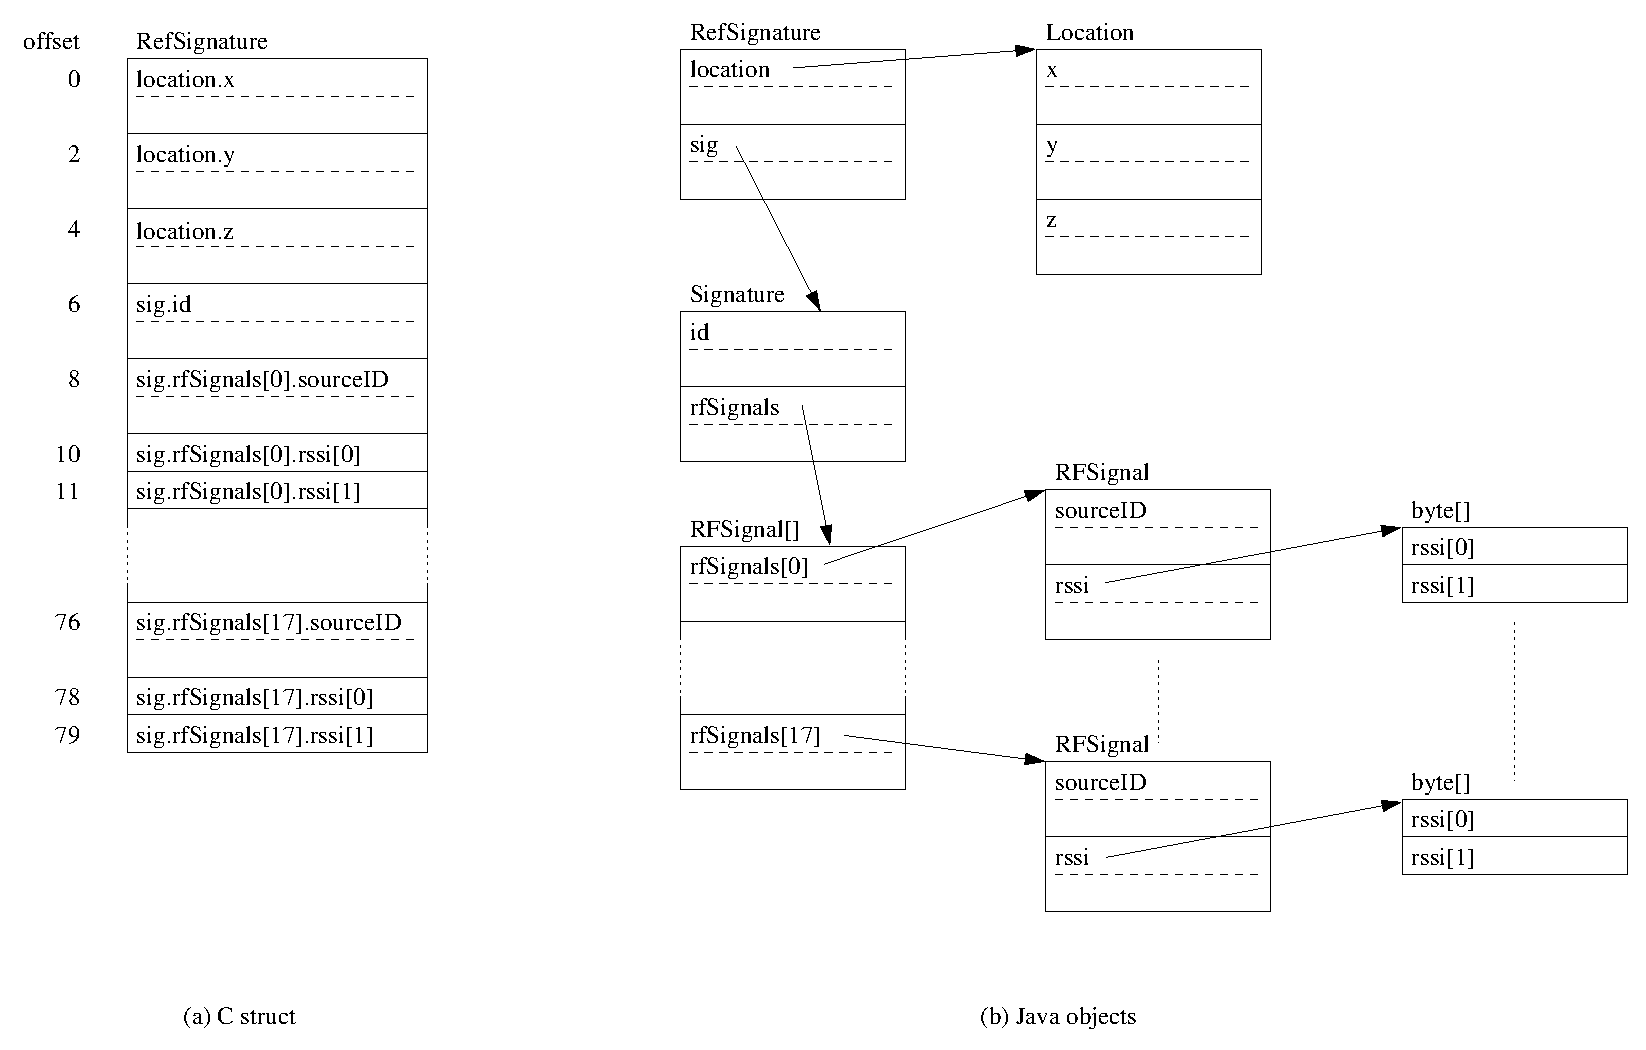
\includegraphics[width=0.9\linewidth]{motetrack-refsignature-objects}
\caption[The \mycode{RefSignature} data structure]{The \mycode{RefSignature} data structure: as a C struct, and as a collection of Java objects}
\label{fig-motetrack-refsignature-objects}
\end{figure}

Since all the arrays are of fixed length, in C the layout of the whole structure is known at compile time, shown in Figure \ref{fig-motetrack-refsignature-objects}.

Java does not have the concept of a struct. As described in Section \ref{sec-background-jvm-memory}, in Java every object is made up of a list of primitive values: either an int or a reference to another object. Thus, the most natural way to translate the C structures in Listing \ref{lst-motetrack-data-structure} to Java, is as a collection of objects and arrays on the heap, as shown in the right half of Figure \ref{fig-motetrack-refsignature-objects}. Note that every one of the 18 \mycode{RFSignal} structs becomes an object, which in turn has a pointer to an array of RSSI values.

There are two problems with this. First, since the location of these Java objects is not known until run time, there is a performance penalty for having to follow the chain of references. \mybench{MoteTrack} will loop over the signals in the \mycode{rfSignals} array. Starting from this array, Java needs to do 3 lookups to get to the right RSSI value: the address of the current \mycode{RFSignal} object, the address of the \mycode{rssi} array, and then the actual RSSI value. For the C version, all the offsets are known at compile time, so the compiler can generate a much more efficient loop, directly reading from the right locations.

The second problem is the added memory usage. The C struct only takes up 80 bytes, all used to store data. The Java version allocates a total of 40 objects, 36 of which are spent on the \mycode{RFSignal} objects and their arrays of RSSI values. Each of these requires a heap header, which takes up 5 bytes. In addition, the 19 arrays have a 3 byte header, and the whole structure contains a total of 39 references, which each take up 2 bytes. In total, the collection of Java objects use $80 + 40*5 + 19*3 + 39*2 = 415$ bytes.

Combined with \mybench{MoteTrack}'s other data structures, this is too large to fit in memory, which forced us to refactor the 2 element \mycode{rssi} array into two byte variable stored directly in \mycode{RFSignal}, as explained in Section \ref{sec-evaluation-benchmark-implementation-motetrack}. This allowed us to run the benchmark, but a RefSignature still takes up 235 bytes, and reading a RSSI value still takes two lookups instead of one.

Generally, large arrays of primitive types do not suffer from this problem and can be stored efficiently, but for programmes containing large arrays of objects this causes significant overhead. In some cases we can work around this problem by flattening the structure, for instance in \mybench{MoteTrack}'s case we could replace the array of \mycode{RFSignal}s with three separate arrays for \mycode{sourceID}s, \mycode{rssi_0} and \mycode{rssi_1}, but only at a significant cost in readability.




\section{Better language support for shorts and bytes}
\label{sec-small-datatypes}
Because RAM is scarce, 16-bit short and single byte data types are commonly used in sensor node code. The standard JVM only has 32 and 64-bit operations, and variables and stack values are stored as 32-bit, even if the actual type is shorter. On a sensor node this wastes memory, and causes a performance overhead since most nodes have 8-bit or 16-bit architectures. Therefore, many sensor node JVMs, including Darjeeling, introduce 16-bit operations and store values in 16-bit slots.

However, this is only one half of the solution. At the language level, Java defines that an expression evaluates to 32-bits, or 64-bits if at least one operand is a \mycode{long}. Attempting to store this in a 16-bit variable will result in a `lossy conversion' error at compile time, unless explicitly cast to a \mycode{short}.

As an example, if we have 3 \mycode{short} variables, a, b, and c, and want to do 
\mycode{a=b+c;}, we need to insert a cast to avoid errors from the Java compiler:

\mycode{a=(short)(b+c);}

Passing literal integer values to a method call treats them as ints, even if they are short enough to fit in a smaller type, which results in calls like: 

\mycode{f((byte)1);}

While seemingly a small annoyance, in more complex code that frequently uses of shorts and bytes, these casts can make the code much harder to read. Table \ref{tbl-quantitative-results} shows that over 25 casts per 100 lines of code can appear in some benchmarks.

\paragraph{Possible solutions}
%If we want to have an efficient sensor node VM, both from a performance and memory usage perspective, better support for data types smaller than 32-bit integers is necessary.

We suggest that C-style automatic narrowing conversions would make most sensor node code more readable, but to leave the option of Java's default behaviour open, we may implement this as new datatypes: declaring variable \mycode{a} as \mycode{unchecked short} would implictly narrow to short when needed, so \mycode{a=b+c;} would not need an explicit cast, while it would if \mycode{a} is declared as a normal \mycode{short}.




\section{Simple type definitions}
\label{sec-typedef}
When developing code for a sensor node, the limited resources often result in different design patterns compared to desktop software. In normal Java code we usually rely on objects for type safety and keeping code readable and easy to maintain. On sensor nodes, objects are expensive and we frequently make use of shorts and ints for a multitude of different tasks for which we would traditionally use objects.

In these situations we often found that our code would be much easier to maintain if there was a way to name new integer types to explicitly indicate their meaning, instead of using many of \mycode{int} or \mycode{short} variables. Having type checking on these types would add a welcome layer of safety.

\paragraph{Possible solutions}
At a minimum, we should have a way to define simple aliases for primitive types, similar to C's \mycode{typedef}. A more advanced option that fits more naturally with Java, would be to have a strict \mycode{typedef} which also does type checking, so that a value of one user defined integer type cannot be accidentally assigned to a variable of another type, without an explicit cast.




\section{Explicit and efficient inlining}
\label{sec-inlining}
Java method calls are inherently more expensive than C functions. On the desktop, JIT compilers can remove much of this overhead, but a sensor node does not have the resources for this. We often found this to be a problem for small helper functions that are frequently called. As an example, the C version of the \mybench{XXTEA} benchmark contains this macro: 

\begin{minted}{c}
    #define MX (((z>>5^y<<2) + (y>>3^z<<4)) \\
                 ^ ((sum^y) + (key[(p&3)^e] ^ z)))
\end{minted}

This macro is called in four places, and is very performance critical. Tools like Proguard \cite{proguard} can be used to inline small methods, but \mycode{MX} is larger than Proguard's size threshold. This leaves developers with two unattractive options: either leaving it as a method and accepting the performance penalty, or manually copy-pasting the code, which is error-prone and leads to code that is harder to maintain.

\paragraph{Possible solutions}
The simplest solution would be to have a preprocessor similar to C's. However, such a low level text-based solution may not be the most user friendly solution for developers without a C background.

Another option is to give the developer more control over inlining, which could easily be achieved by adding an \mycode{inline} keyword to force the compiler to inline important methods.

% These annotations are usually placed at the method level. As an extension, since not all calls may be equally important for performance, it may be useful allow the developer to save code space by placing the \mycode{inline} keyword at a call instead of at the method level to only inline specific, performance sensitive calls.




\section{An optimising compiler}
\label{sec-optimising-javac}
As discussed in previous chapters, but listed here again for completeness, Java compilers typically do not optimise the bytecode but translate the source almost as-is. Without a clear performance model it is not always clear which option is faster, and the bytecode is expected to be run by a JIT compiler, which can make better optimisation decisions knowing the target platform and run-time behaviour. However, a sensor node does not have the resources for this and must execute the code as it is received. This leads to significant overhead, for example by repeatedly reevaluating a constant expression in a loop.

\paragraph{Possible solutions}
Even without a clear performance model, some basic optimisations can be done. The results in Section \ref{sec-evaluation-manual-optimisations} show that some very conservative optimisations can already result in code twice as fast as the original. These could be further expanded, and combining the tasks of the optimiser and infuser can further improve performance as shown in Section \ref{sec-evaluation-other-platforms-word-size}.




\section{Allocating objects on stack}
\label{sec-no-gc}
In Java anything larger than a primitive value has to be allocated on the heap. This introduces a performance overhead, both for allocating the objects, and the occasional run of the garbage collector that may take several thousand cycles.

In our benchmarks we encountered a number of situations where a temporary object was needed. For example, the \mycode{encode} function in the \mybench{LEC} benchmark needs to return two values: \emph{bsi} and the number of bits in \emph{bsi}. In C this is done by passing two pointers to \mycode{encode}. In Java we can wrap both values in a class and either create and return an object from \mycode{encode}, or let the caller create it and pass it as a parameter for \mycode{encode} to fill in.

In code that frequently needs short-lived objects the overhead for allocating them can be significant, and unpredictable garbage collector runs are a problem for code with specific timing constraints. Besides \mybench{LEC}, we saw similar situations in the \mybench{CoreMark}, \mybench{MoteTrack} and \mybench{Heat detection} benchmarks. The problem is especially serious on a sensor node, where the limited amount of memory means the garbage collector is triggered frequently even if relatively few temporary objects are created.

\begin{listing}
\begin{minted}{java}
    public static short LEC(short[] numbers, Stream stream) {
        BSI bsi = new BSI();      // Allocate bsi only once
        for (...) {
            ...
            compress(ri, ri_1, stream, bsi);
            ...
        }
    }

    private static void compress(short ri, short ri_1, Stream stream, BSI bsi) {
        ...
        encode(di, bsi);          // Pass bsi to encode to return both value and length
        ...
    }

    private static void encode(short di, BSI bsi) {
        ...
        bsi.value = ...           // return value and length by setting object fields
        bsi.length = ...
    }
\end{minted}
\caption{Avoiding multiple object allocations in the LEC benchmark}
\label{lst-lec-avoiding-object-allocations}
\end{listing}

This overhead can often be reduced by allocating earlier and reusing the same objects in a loop. In Listing \ref{lst-lec-avoiding-object-allocations} we see this implemented for the \mybench{LEC} benchmark, where we use the \mycode{bsi} object to return two values from \mycode{encode} to \mycode{compress}. Instead of creating a new object in each iteration in the \mycode{compress} method where it is needed, we create \mycode{bsi} once, outside of the main loop, and pass the same object to \mycode{compress} multiple times.

This technique of pulling object creation up the call chain can often be used to remove this sort of overhead, and it worked in all four benchmarks mentioned before. However, it gets very cumbersome if the number of objects is more than one or two, or if they need to be passed through multiple layers. Readability is also reduced, since objects that are only needed in a specific location are now visible from a much larger scope.

\paragraph{Possible solutions}
On desktop JVMs, escape analysis \cite{Choi:1999uw, Goetz:2005uy} is used to determine if an object can be safely allocated on the stack instead of the heap, thus saving both the cost of heap allocation, and the occasional garbage collection run triggered by it.

While the analysis of the bytecode required for this is far too complex for a sensor node, it could be done offline, similar to TakaTuka's offline garbage collector analysis. The bytecode can then be extended by adding special versions of the \mycode{new} opcodes to instruct the VM to place an object in the stack frame instead of the heap. A field should also be added to the method header to tell the VM how much extra space for stack objects needs to be reserved in the stack frame.

There is a risk to doing this automatically. In our sensor node VM, the split between heap and stack memory is fixed, and both are limited. If the compiler automatically puts all objects that could be on the stack in the stack frame instead of the heap, we may end up with an empty heap, and a stack overflow. Therefore, it is better to leave this optimisation to the developer by also introducing a new keyword at the language level, so developers can explicitly indicate which objects go on the stack and which in the heap. Of course escape analysis is still necessary to check at compile time this keyword is only used in places where it is legal for the object to be allocated on the stack.




\section{Reconsidering advanced language features}
\label{sec-advanced-features}
Finally, we conclude with some discussion on more fundamental language design choices. Many sensor node JVMs implement some of Java's more advanced features, but we are not convinced this is always a good choice on a sensor node.

While features like threads and garbage collection are all useful, they come at a cost. The trade-off for a sensor node VM is significantly different from a desktop VM: many of Java's more advanced features are vital to large-scale software development, but the size of sensor nodes programmes is much smaller. And while VM size is not an issue on the desktop, these features are relatively expensive to implement on a sensor node with limited flash memory. We believe a VM developed from scratch, with the aim of providing platform independence, safety, and performance through AOT compilation, would end up with a design very different from the JVM.

Table \ref{tab-vm-size} shows the code size in Darjeeling for some features we discuss below. This was determined by only counting the size of functions directly related to specific features. The actual cost is higher since some, especially garbage collection, also add complexity to other functions throughout the VM. Combined, the features below and the string functions mentioned in Section \ref{sec-std-lib} make up about half the original Darjeeling VM.

Besides an increase in VM size, these features also cause a performance penalty, and features such as threads and exceptions are much harder in an AOT compiler where we cannot implement them in the interpreter loop. This means that if we care about performance and the corresponding reduction in CPU energy consumption, we either have to give them up, or spend considerably more in terms of VM complexity and size.


\subsection{Threads}
As shown in Table \ref{tab-vm-size}, support for threads accounts for about 10\% of the VM size, if we exclude the string library. In addition, each thread requires a stack. If we allocate a fixed block, it must be large enough to avoid stack overflows, but too large a block wastes precious RAM. Darjeeling allocates each stack as a linked list of frames on the heap. This is memory efficient, but allocating on the heap is slower and will occasionally trigger the garbage collector.

A more cooperative concurrency model is more appropriate for sensor nodes, where lightweight tasks voluntarily yield the CPU and share a single stack. This is also the approach to concurrency chosen by a number of native code systems, including \emph{t-kernel} \cite{Gu:2005un}, nesC \cite{Gay:2003up}, and more recently Amulet \cite{Hester:2016je}.


\subsection{Exceptions}
In terms of code size, exceptions are not very expensive to implement in an interpreter, but they are hard to implement in an AOT compiler. We also feel the advantage of having exceptions is much lower than the other features mentioned in this section, since they could be easily replaced with return values to signal errors.


\subsection{Virtual methods}
It is hard to quantify the overhead of implementing virtual methods since the code for handling them is integrated into several functions. In terms of size it is likely less than 2 KB, but the performance overhead is considerable. The target of a virtual method call must be resolved at run time, they cannot be made lightweight, and an AOT compiler can generate much more efficient code for calls to static methods.

In practice we seldom use virtual methods in sensor node code, but some form of indirect calls is necessary for things like signal handling. It should be possible to develop a more lightweight form of function pointers that can be implemented efficiently. However, the details will require more careful study.


\subsection{Garbage collection}
Finally, garbage collection is clearly the most intrusive aspect of the JVM to change. While the first three features could be changed with minor modifications to Java, the managed heap is at its very core.

Still, there are good reasons for considering alternatives. Table \ref{tab-vm-size} shows the garbage collector functions in Darjeeling add up to about 3.5 KB, but the actual cost is much higher as many other parts of Darjeeling are influenced by the garbage collector.

Specifically, it is the reason Darjeeling splits references and integers throughout the VM. This makes it easy for the garbage collector to find live references, but leads to significant code duplication and complexity. Using AOT compilation, the split stack adds overhead to maintain this state, and requires two extra registers as a second stack pointer that cannot be used for stack caching.




\section{Building better sensor node VMs}
In this chapter we described a number of issues we encountered over the years while using and developing sensor node VMs. They may not apply to every scenario, but the wide range of the issues presented here suggests many applications will be affected by at least some.

Most sensor node VMs already modify the instruction set of the original VM and usually support only a subset of the original language. The issues described here indicate these changes do not go far enough, and we still need to refine our VMs further to make them truly useful in real-world projects.

There are two possible paths to follow: a number of issues can be solved by improving existing Java-based VMs. Staying close to Java has the advantage of being able to reuse existing knowledge and infrastructure.

However some of the issues require more invasive changes to both the source language and VM. If the goal is to run platform independent code safely and efficiently, rather than running Java, we should start from the specific requirements and constraints of sensor node software development, which would lead to more lightweight features and a more predictable memory model.

For either path, we hope the points presented in this chapter can help in the development of better future sensor node VMs.

\chapter{Conclusion}
A major problem for sensor node VMs has been performance. Most interpreters are between one to two orders of magnitude slower than native code, leading to both lower maximum throughput and increased energy consumption.

Previous work on AOT translation to native code by Ellul and Martinez \cite{Ellul:2010iw} improves performance, but still a significant overhead remains, and the tradeoff is that the resulting native code takes up much more space, limiting the size of programmes that can be loaded onto a device. For the CoreMark benchmark, the performance is 9x slower than native C, and the code 3.5 times larger.

In this paper, we presented the complete set of techniques we developed to mitigate this code size overhead and to further improve performance. We evaluated their effectiveness using a set of benchmarks, some with specific characteristics to highlight the results in more extreme conditions, and include the larger CoreMark benchmark to represent the average behaviour of larger sensor node applications. Combined, our optimisations result in a compiler that produces code that is on average only 1.7 times slower and 1.9 times larger than optimised C.

These optimisations do increase the size of our VM, but the break-even point at which this is compensated for by the smaller code it generates, is well within the range of programme memory typically available on a sensor node. This leads us to believe that these optimisations will be useful in many scenarios, and make using a VM a viable option for a wider range of applications.

Many opportunities for future work remain. In this paper we focus on techniques for the sensor node side, but a future VM should come with a better optimising infuser on the host to prepare better quality bytecode. This infuser should also support inlining small methods as efficiently as manual inlining, and in most cases automatically determine which methods should be made lightweight.

For the mark loops optimisation, a heuristic is needed to make a better decision on the number of registers to pin, and we can consider applying this optimisation to other blocks that have a single point of entry and exit as well. Since supporting preemptive threads is expensive to implement without the interpreter loop as a place to switch threads, we believe a cooperative concurrency model where threads explicitly yield control is more suitable for sensor nodes using AOT, and we are working on building this on top of Darjeeling's existing thread support.

A more general question is what the most suitable architecture and instruction set is for a VM on tiny devices. Hsieh et al. note that the performance problem lies in the mismatch between the VM and the native machine architecture \cite{Hsieh:1996cy}. In this paper we presented a number of modifications to the bytecode format to make it better suited for use on a sensor now, but ultimately we believe JVM is not the best choice for a sensor node VM. It has some advanced features, such as exceptions, preemptive threads, and garbage collection, which add complexity but may not be necessary on a tiny device. At the same time, there is no support for constant data, which is common in embedded code: a table with sine wave values in the fft benchmark is represented as a normal array at run-time, using up valuable memory.
% In the case of CoreMark this forced us to convert some arrays of constant data used to check the benchmark results, into a function with a large \mycode{switch} statement that returns the right value.
We may also consider extending the bytecode with instructions to express common operations more efficiently. For example, an instruction to loop over an array such as the one found in Lua \cite{Lua:2005} would allow us to generate more efficient code and eliminate most of the remaining overhead in the bubble sort benchmark.
% TODO Suganuma seems to propose something similar


Our reason to use JVM is the availability of a lot of infrastructure to build on. Like Hsieh et al., we do not claim that Java is the best answer for a sensor node VM, but we believe the techniques presented here will be useful in developing better sensor node VMs, regardless of the exact instruction set used.

One important question that should be considered is whether that instruction set should be stack-based or register-based. Many modern bytecode formats are register-based, and a number of publications report on the advantages of this approach \cite{Zhang:2012wf, Shi:2005ba}. However, these tradeoffs are quite different for a powerful JIT compiler, and a resource-constrained VM. When working with tiny devices, an important advantage of a stack-based architecture is its simplicity, and our results here show that much of the overhead associated with the stack-based approach can be eliminated during the translation process.



%TODO Mention CoreMark on desktop numbers here. Nice point to end the paper on (although it's not a fair comparison since the desktop version does things like bounds checking)

%TODO point to make somewhere: more complex techniques could possibly improve results further, but will cost more. 2x slowdown seems acceptable. there's always a tradeoff and we needs several datapoints to make a choice. this work shows we can achieve a lot with very little, but we may be able to achieve even more at a greater cost.

%TODO: subsubsection and paragraph look very similar, maybe only use one?
%TODO: consistent table layout. double midrule to separate header from body
%TODO: consistent placement of label for figures and tables and listings


\appendix

\backmatter

\addcontentsline{toc}{chapter}{\bibname}
\bibliographystyle{abbrv}

% Your bibliography goes here
\bibliography{references}

\end{document}
